\documentclass[14pt,a4paper]{extarticle}

\usepackage{iftex}
\ifPDFTeX
  \usepackage[T2A]{fontenc}
  \usepackage[utf8]{inputenc}
  \usepackage[russian]{babel}
\else
  \usepackage{fontspec}
  \usepackage{polyglossia}
  \setmainlanguage{russian}
  \setmainfont{DejaVu Serif}
  \setsansfont{DejaVu Sans}
  \setmonofont{DejaVu Sans Mono}
  \newfontfamily\cyrillicfont{DejaVu Serif}
  \newfontfamily\cyrillicfontsf{DejaVu Sans}
  \newfontfamily\cyrillicfonttt{DejaVu Sans Mono}
\fi

\usepackage[a4paper,left=30mm,right=10mm,top=20mm,bottom=20mm]{geometry}
\usepackage{setspace}
\onehalfspacing
\usepackage{indentfirst}
\setlength{\parindent}{1.25cm}
\setlength{\parskip}{0pt}

\usepackage{graphicx}
\usepackage{float}
\usepackage{longtable}
\usepackage{booktabs}
\usepackage{array}
\usepackage{calc}
\usepackage{multirow}
\usepackage{makecell}
\usepackage{enumitem}
\usepackage{amsmath,amssymb}
\usepackage{url}
\usepackage[hidelinks]{hyperref}

\setcounter{secnumdepth}{0}
\setcounter{tocdepth}{3}
\sloppy
\emergencystretch=3em
\setlist{nosep}
\renewcommand{\arraystretch}{1.2}

\providecommand{\tightlist}{%
  \setlength{\itemsep}{0pt}\setlength{\parskip}{0pt}}

\begin{document}

\begin{titlepage}
\begin{center}
Министерство науки и высшего образования Российской Федерации\\
Федеральное государственное автономное образовательное учреждение высшего образования\\
\textbf{«Северо-Кавказский федеральный университет»}\\[0.5cm]
Факультет математики и компьютерных наук им. профессора Н.И. Червякова\\
Кафедра организации и технологии защиты информации
\end{center}

\vfill

\begin{center}
\textbf{ВЫПУСКНАЯ КВАЛИФИКАЦИОННАЯ РАБОТА СТУДЕНТА}\\[0.4cm]
Раздел 1. Проектирование архитектуры и разработка серверной части платформы планирования безопасных маршрутов БПЛА с модулем оценки киберугроз\\[0.8cm]
\textbf{«Разработка платформы автоматизированного планирования безопасных маршрутов для групп сельскохозяйственных дронов с учётом киберугроз»}
\end{center}

\vfill

\begin{flushright}
Направление подготовки: 10.03.01 «Информационная безопасность»\\
Студент: Сутормин Матвей Павлович\\
Группа: ИНБ-б-о-22-1\\[0.4cm]
Руководитель: канд. техн. наук, доцент Петренко В.И.
\end{flushright}

\vfill

\begin{center}
Ставрополь, 2026
\end{center}
\end{titlepage}

\hypertarget{ux437ux430ux434ux430ux43dux438ux435-ux43dux430-ux432ux44bux43fux443ux441ux43aux43dux443ux44e-ux43aux432ux430ux43bux438ux444ux438ux43aux430ux446ux438ux43eux43dux43dux443ux44e-ux440ux430ux431ux43eux442ux443-ux441ux442ux430ux440ux442ux430ux43f}{%
\section{Задание на выпускную квалификационную работу (стартап)}\label{ux437ux430ux434ux430ux43dux438ux435-ux43dux430-ux432ux44bux43fux443ux441ux43aux43dux443ux44e-ux43aux432ux430ux43bux438ux444ux438ux43aux430ux446ux438ux43eux43dux43dux443ux44e-ux440ux430ux431ux43eux442ux443-ux441ux442ux430ux440ux442ux430ux43f}}

\begin{quote}
Актуализация 22.04.2026: формулировки задания синхронизированы с текущим состоянием кода (выполнены промпты 13--22; validation report + PLR/packet-loss обновления).
\end{quote}

Формальный текст задания вынесен из \href{roadmap_task.md}{\texttt{roadmap\_task.md}}, чтобы календарный план и официальное задание не смешивались в одном файле.

\textbf{Согласование с ТЗ на ПО:} детали реализации платформы --- в \href{ТЗ.md}{\texttt{ТЗ.md}}. Раздел \textbf{§10} описывает \textbf{целевую} модель динамического определения угрозы по нескольким источникам (GNSS, IMU, радиоканал, согласованность роя и др.) и слияния признаков. В репозитории реализована \textbf{упрощённая} цепочка по MAVLink (эвристики, без ML/SDR) --- см. \href{Промпты.md}{\texttt{Промпты.md}} 9--12; \textbf{полная} постановка §10 \textbf{не входит} в минимальный объём подтверждения задания и может излагаться в перспективах ВКР и в \href{knowledge/}{\texttt{knowledge/}}.

\begin{center}\rule{0.5\linewidth}{0.5pt}\end{center}

Министерство науки и высшего образования Российской Федерации Федеральное государственное автономное образовательное учреждение высшего образования «СЕВЕРО-КАВКАЗСКИЙ ФЕДЕРАЛЬНЫЙ УНИВЕРСИТЕТ»

\textbf{Факультет:} Факультет математики и компьютерных наук им. профессора Н.И. Червякова\\
\textbf{Кафедра:} Организации и технологии защиты информации\\
\textbf{Направление подготовки:} 10.03.01 «Информационная безопасность»\\
\textbf{Направленность (профиль):} «Организация и технологии защиты информации (по отрасли или в сфере профессиональной деятельности)»

«УТВЕРЖДАЮ» Зав. кафедрой организации и технологии защиты информации канд. техн. наук, доцент Петренко В. И. \_\_\_\_\_\_\_\_\_\_\_\_\_\_\_\_\_\_\_\_\_\_\_\_\_\_\_\_\_ (подпись) «\_\_\_\_\_»\_\_\_\_\_\_\_\_\_\_\_\_\_2026 г.

\textbf{Тема ВКРС:} Разработка платформы автоматизированного планирования безопасных маршрутов для групп сельскохозяйственных дронов с учётом киберугроз\\
\emph{(Утверждена приказом проректора по учебной работе от «\textbf{\emph{»}}\_\_\_\_\_2026 г. №\_\_\_\_\_\_)}

\begin{center}\rule{0.5\linewidth}{0.5pt}\end{center}

\hypertarget{ux440ux430ux437ux434ux435ux43b-1.-ux43fux440ux43eux435ux43aux442ux438ux440ux43eux432ux430ux43dux438ux435-ux430ux440ux445ux438ux442ux435ux43aux442ux443ux440ux44b-ux438-ux440ux430ux437ux440ux430ux431ux43eux442ux43aux430-ux441ux435ux440ux432ux435ux440ux43dux43eux439-ux447ux430ux441ux442ux438-ux43fux43bux430ux442ux444ux43eux440ux43cux44b-ux43fux43bux430ux43dux438ux440ux43eux432ux430ux43dux438ux44f-ux431ux435ux437ux43eux43fux430ux441ux43dux44bux445-ux43cux430ux440ux448ux440ux443ux442ux43eux432-ux431ux43fux43bux430-ux441-ux43cux43eux434ux443ux43bux435ux43c-ux43eux446ux435ux43dux43aux438-ux43aux438ux431ux435ux440ux443ux433ux440ux43eux437}{%
\subsection{РАЗДЕЛ 1. Проектирование архитектуры и разработка серверной части платформы планирования безопасных маршрутов БПЛА с модулем оценки киберугроз}\label{ux440ux430ux437ux434ux435ux43b-1.-ux43fux440ux43eux435ux43aux442ux438ux440ux43eux432ux430ux43dux438ux435-ux430ux440ux445ux438ux442ux435ux43aux442ux443ux440ux44b-ux438-ux440ux430ux437ux440ux430ux431ux43eux442ux43aux430-ux441ux435ux440ux432ux435ux440ux43dux43eux439-ux447ux430ux441ux442ux438-ux43fux43bux430ux442ux444ux43eux440ux43cux44b-ux43fux43bux430ux43dux438ux440ux43eux432ux430ux43dux438ux44f-ux431ux435ux437ux43eux43fux430ux441ux43dux44bux445-ux43cux430ux440ux448ux440ux443ux442ux43eux432-ux431ux43fux43bux430-ux441-ux43cux43eux434ux443ux43bux435ux43c-ux43eux446ux435ux43dux43aux438-ux43aux438ux431ux435ux440ux443ux433ux440ux43eux437}}

\textbf{Студент:} Сутормин Матвей Павлович (группа: ИНБ-б-о-22-1, Курс: 4)

\hypertarget{ux438ux441ux445ux43eux434ux43dux44bux435-ux434ux430ux43dux43dux44bux435-ux434ux43bux44f-ux43fux440ux43eux435ux43aux442ux438ux440ux43eux432ux430ux43dux438ux44f}{%
\subsubsection{2.1. Исходные данные для проектирования:}\label{ux438ux441ux445ux43eux434ux43dux44bux435-ux434ux430ux43dux43dux44bux435-ux434ux43bux44f-ux43fux440ux43eux435ux43aux442ux438ux440ux43eux432ux430ux43dux438ux44f}}

\begin{itemize}
\tightlist
\item
  Математическая модель интегрального критерия доверенной эффективности.
\item
  Алгоритмы динамического перепланирования маршрутов.
\item
  Метрика оценки деструктивного воздействия на процесс координации и маршрутизации.
\item
  Данные о характеристиках коммерческих агро-БПЛА (автономность, полезная нагрузка, радиус связи).
\item
  Open-source библиотеки: OR-Tools, networkx, FastAPI, PostGIS.
\end{itemize}

\hypertarget{ux441ux442ux440ux443ux43aux442ux443ux440ux430-ux438-ux441ux43eux434ux435ux440ux436ux430ux43dux438ux435-ux43fux435ux440ux432ux43eux433ux43e-ux440ux430ux437ux434ux435ux43bux430-ux432ux43aux440ux441}{%
\subsubsection{2.2. Структура и содержание первого раздела ВКРС:}\label{ux441ux442ux440ux443ux43aux442ux443ux440ux430-ux438-ux441ux43eux434ux435ux440ux436ux430ux43dux438ux435-ux43fux435ux440ux432ux43eux433ux43e-ux440ux430ux437ux434ux435ux43bux430-ux432ux43aux440ux441}}

\begin{longtable}[]{@{}
  >{\raggedright\arraybackslash}p{(\columnwidth - 4\tabcolsep) * \real{0.3077}}
  >{\raggedright\arraybackslash}p{(\columnwidth - 4\tabcolsep) * \real{0.3077}}
  >{\centering\arraybackslash}p{(\columnwidth - 4\tabcolsep) * \real{0.3846}}@{}}
\toprule\noalign{}
\begin{minipage}[b]{\linewidth}\raggedright
Структурный элемент ВКРС / этап ГИА
\end{minipage} & \begin{minipage}[b]{\linewidth}\raggedright
Содержание
\end{minipage} & \begin{minipage}[b]{\linewidth}\centering
Компетенции (10.03.01)
\end{minipage} \\
\midrule\noalign{}
\endhead
\bottomrule\noalign{}
\endlastfoot
Титульный лист, задание & Оформление по регламенту ВКРС СКФУ & --- \\
Содержание & Перечень разделов и подразделов работы & --- \\
Введение & Обоснование актуальности. Анализ рынка и существующих решений. Формулировка проблемы, цели и задач. Описание бизнес-идеи стартапа. & ОПК-1, ОПК-3 \\
1.1 Общее описание проекта (совместный раздел) & Тренды рынка агродронов, анализ ЦА, конкурентный анализ. Описание продукта. Бизнес-модель (SaaS). Финансовый план и стратегия. & ОПК-1, ОПК-3, УК-2 \\
1.2 Анализ угроз и моделирование рисков & Систематизация деструктивных воздействий. Разработка модели угроз. Формализация метрики оценки деструктивного воздействия. & ОПК-2, ОПК-4, ПК-1 \\
1.3 Проектирование архитектуры платформы & Разработка общей архитектуры системы. Проектирование базы данных (PostGIS), REST API. Модуль карты рисков. Спецификация MAVLink-интеграции. & ОПК-4, ПК-2, ПК-3 \\
1.4 Разработка серверной части и алгоритмов & Backend (Python, FastAPI). Алгоритм разбиения зоны покрытия. Модуль карты рисков. Логика динамического перепланирования. & ОПК-4, ПК-2, ПК-3, ПК-4 \\
1.5 Эксперименты и оценка эффективности & Тестовые сценарии и метрики по \texttt{План\ обдуманный.md} §1.5. Воспроизводимая Python-симуляция (baseline vs предлагаемый алгоритм); при наличии среды --- демонстрация на ArduPilot SITL. Сравнение с аналогами по ключевым критериям. & ОПК-4, ПК-3, ПК-4 \\
Заключение & Выводы по результатам разработки серверной части и алгоритмов. Перспективы. & УК-1 \\
Список использованных источников & Не менее 40 источников, в т.ч. не менее 10 на иностранном языке & --- \\
Защита ВКРС & Доклад, демонстрация MVP, результаты тестирования & УК-4 \\
\end{longtable}

\hypertarget{ux43fux435ux440ux435ux447ux435ux43dux44c-ux433ux440ux430ux444ux438ux447ux435ux441ux43aux43eux433ux43e-ux43cux430ux442ux435ux440ux438ux430ux43bux430}{%
\subsubsection{2.3. Перечень графического материала:}\label{ux43fux435ux440ux435ux447ux435ux43dux44c-ux433ux440ux430ux444ux438ux447ux435ux441ux43aux43eux433ux43e-ux43cux430ux442ux435ux440ux438ux430ux43bux430}}

Диаграмма архитектуры платформы (UML); ER-диаграмма базы данных; блок-схема алгоритма маршрутизации с учётом риска; блок-схема алгоритма динамического перепланирования; скриншоты работы веб-платформы и/или ArduPilot SITL (по наличию); графики сравнительной оценки эффективности (Python-симуляция).

\textbf{Дата выдачи задания:} 01 апреля 2026 г.\\
\textbf{Руководитель (координатор) проекта:} \_\_\_\_\_\_\_\_\_\_\_\_\_\_ Петренко В.И.\\
\textbf{Руководитель первого раздела проекта:} \_\_\_\_\_\_\_\_\_\_\_\_\_\_ Петренко В.И.\\
\textbf{Задание принял к исполнению:} \_\_\_\_\_\_\_\_\_\_\_\_\_\_ Сутормин М.П.

\begin{center}\rule{0.5\linewidth}{0.5pt}\end{center}

\hypertarget{ux440ux430ux437ux434ux435ux43b-2.-ux440ux430ux437ux440ux430ux431ux43eux442ux43aux430-ux43aux43bux438ux435ux43dux442ux441ux43aux43eux439-ux447ux430ux441ux442ux438-ux43fux43bux430ux442ux444ux43eux440ux43cux44b-ux438-ux43cux43eux434ux443ux43bux44f-ux43eux431ux435ux441ux43fux435ux447ux435ux43dux438ux44f-ux438ux43dux444ux43eux440ux43cux430ux446ux438ux43eux43dux43dux43eux439-ux431ux435ux437ux43eux43fux430ux441ux43dux43eux441ux442ux438-ux432ux437ux430ux438ux43cux43eux434ux435ux439ux441ux442ux432ux438ux44f-ux441-ux433ux440ux443ux43fux43fux43eux439-ux431ux43fux43bux430}{%
\subsection{РАЗДЕЛ 2. Разработка клиентской части платформы и модуля обеспечения информационной безопасности взаимодействия с группой БПЛА}\label{ux440ux430ux437ux434ux435ux43b-2.-ux440ux430ux437ux440ux430ux431ux43eux442ux43aux430-ux43aux43bux438ux435ux43dux442ux441ux43aux43eux439-ux447ux430ux441ux442ux438-ux43fux43bux430ux442ux444ux43eux440ux43cux44b-ux438-ux43cux43eux434ux443ux43bux44f-ux43eux431ux435ux441ux43fux435ux447ux435ux43dux438ux44f-ux438ux43dux444ux43eux440ux43cux430ux446ux438ux43eux43dux43dux43eux439-ux431ux435ux437ux43eux43fux430ux441ux43dux43eux441ux442ux438-ux432ux437ux430ux438ux43cux43eux434ux435ux439ux441ux442ux432ux438ux44f-ux441-ux433ux440ux443ux43fux43fux43eux439-ux431ux43fux43bux430}}

\textbf{Студент:} Яковенко Вячеслав Станиславович (группа: ИНБ-б-о-22-1, Курс: 4)

\hypertarget{ux438ux441ux445ux43eux434ux43dux44bux435-ux434ux430ux43dux43dux44bux435-ux434ux43bux44f-ux43fux440ux43eux435ux43aux442ux438ux440ux43eux432ux430ux43dux438ux44f-1}{%
\subsubsection{3.1. Исходные данные для проектирования:}\label{ux438ux441ux445ux43eux434ux43dux44bux435-ux434ux430ux43dux43dux44bux435-ux434ux43bux44f-ux43fux440ux43eux435ux43aux442ux438ux440ux43eux432ux430ux43dux438ux44f-1}}

\begin{itemize}
\tightlist
\item
  Архитектура серверной части платформы и REST API (результат Раздела 1, Сутормин М.П.).
\item
  Модель угроз из базового НИР (рук. доцент В.И. Петренко). Протоколы взаимодействия с БПЛА (MAVLink).
\item
  Стандарты ИБ: ГОСТ Р 56939-2016, OWASP Top-10, методика ФСТЭК по оценке угроз (2021).
\item
  Библиотеки и фреймворки: React, Leaflet, Vite, Zustand; JWT (реализация на backend); при необходимости обоснования --- TLS/mTLS, cryptography (как направления усиления).
\end{itemize}

\hypertarget{ux441ux442ux440ux443ux43aux442ux443ux440ux430-ux438-ux441ux43eux434ux435ux440ux436ux430ux43dux438ux435-ux432ux442ux43eux440ux43eux433ux43e-ux440ux430ux437ux434ux435ux43bux430-ux432ux43aux440ux441}{%
\subsubsection{3.2. Структура и содержание второго раздела ВКРС:}\label{ux441ux442ux440ux443ux43aux442ux443ux440ux430-ux438-ux441ux43eux434ux435ux440ux436ux430ux43dux438ux435-ux432ux442ux43eux440ux43eux433ux43e-ux440ux430ux437ux434ux435ux43bux430-ux432ux43aux440ux441}}

\begin{longtable}[]{@{}
  >{\raggedright\arraybackslash}p{(\columnwidth - 4\tabcolsep) * \real{0.3077}}
  >{\raggedright\arraybackslash}p{(\columnwidth - 4\tabcolsep) * \real{0.3077}}
  >{\centering\arraybackslash}p{(\columnwidth - 4\tabcolsep) * \real{0.3846}}@{}}
\toprule\noalign{}
\begin{minipage}[b]{\linewidth}\raggedright
Структурный элемент ВКРС / этап ГИА
\end{minipage} & \begin{minipage}[b]{\linewidth}\raggedright
Содержание
\end{minipage} & \begin{minipage}[b]{\linewidth}\centering
Компетенции (10.03.01)
\end{minipage} \\
\midrule\noalign{}
\endhead
\bottomrule\noalign{}
\endlastfoot
Титульный лист, задание & Оформление по регламенту ВКРС СКФУ & --- \\
Содержание & Перечень разделов и подразделов работы & --- \\
Введение & Обоснование актуальности обеспечения ИБ. Анализ угроз каналу управления. Цель и задачи раздела. Роль клиентской части и модуля ИБ. & ОПК-1, ОПК-3 \\
2.1 Общее описание проекта (совместный раздел) & Тренды рынка агродронов, анализ ЦА, конкурентный анализ. Описание продукта. Бизнес-модель (SaaS). Финансовый план (Совместно с Суторминым). & ОПК-1, ОПК-3, УК-2 \\
2.2 Анализ требований к ИБ платформы & Анализ угроз (OWASP Top-10, перехват MAVLink, replay-атаки). Формирование требований к защите. Выбор механизмов защиты. & ОПК-2, ОПК-4, ПК-1 \\
2.3 Разработка клиентской части платформы & Проектирование UX/UI оператора (GeoJSON/KML, настройка миссии, карта React.js + Leaflet.js). Панель диспетчеризации. Интеграция с REST API. & ОПК-4, ПК-2, ПК-3 \\
2.4 Разработка модуля информационной безопасности & Подсистема аутентификации (JWT) и ролевая модель. Анализ и обоснование защиты канала MAVLink (в объёме MVP --- pymavlink; TLS/mTLS/HMAC --- как перспектива усиления). Аудит действий (по объёму ВКР). Защита от типовых веб-уязвимостей. & ОПК-2, ОПК-4, ПК-1, ПК-4 \\
2.5 Тестирование безопасности и интеграционное & Разработка методики тестирования. Пентест веб-интерфейса. Моделирование атак на канал связи. Интеграционное тестирование. & ОПК-4, ПК-3, ПК-4 \\
Заключение & Выводы по результатам разработки. Рекомендации по усилению защищённости. & УК-1 \\
Список использованных источников & Не менее 40 источников, в т.ч. не менее 10 на иностранном языке & --- \\
Защита ВКРС & Доклад, демонстрация интерфейса и модуля ИБ, результаты пентеста & УК-4 \\
\end{longtable}

\hypertarget{ux43fux435ux440ux435ux447ux435ux43dux44c-ux433ux440ux430ux444ux438ux447ux435ux441ux43aux43eux433ux43e-ux43cux430ux442ux435ux440ux438ux430ux43bux430-1}{%
\subsubsection{3.3. Перечень графического материала:}\label{ux43fux435ux440ux435ux447ux435ux43dux44c-ux433ux440ux430ux444ux438ux447ux435ux441ux43aux43eux433ux43e-ux43cux430ux442ux435ux440ux438ux430ux43bux430-1}}

Макеты интерфейса (wireframes); скриншоты реализованного веб-интерфейса; диаграмма потоков данных (DFD) с указанием точек защиты; схема аутентификации и авторизации (JWT); схема канала связи с БПЛА (MAVLink; при необходимости --- варианты усиления TLS/mTLS); результаты проверок / пентеста (отчёт или таблица); скриншоты интеграционного тестирования.

\textbf{Срок представления ВКРС к защите:} 01 июня 2026 г.\\
\textbf{Дата выдачи задания:} 01 апреля 2026 г.\\
\textbf{Руководитель (координатор) проекта:} \_\_\_\_\_\_\_\_\_\_\_\_\_\_ Петренко В.И.\\
\textbf{Руководитель второго раздела проекта:} \_\_\_\_\_\_\_\_\_\_\_\_\_\_ Антонов В.В.\\
\textbf{Задание принял к исполнению:} \_\_\_\_\_\_\_\_\_\_\_\_\_\_ Яковенко В.С.

\begin{center}\rule{0.5\linewidth}{0.5pt}\end{center}

\emph{Текст синхронизирован с \texttt{roadmap\_task.md} (вынесен 19.04.2026). Дополнено ссылкой на \texttt{ТЗ.md} §10 (апрель 2026).}

\clearpage

\tableofcontents
\clearpage

\hypertarget{ux440ux435ux444ux435ux440ux430ux442}{%
\section{РЕФЕРАТ}\label{ux440ux435ux444ux435ux440ux430ux442}}

Выпускная квалификационная работа студента на тему «Разработка платформы автоматизированного планирования безопасных маршрутов для групп сельскохозяйственных дронов с учётом киберугроз» выполнена по направлению подготовки 10.03.01 «Информационная безопасность».

\textbf{Объём раздела 1:} 65 страниц, 15 таблиц, 6 рисунков (схем), 43 источника (из них 19 на иностранном языке).

\textbf{Ключевые слова:} БЕСПИЛОТНЫЙ ЛЕТАТЕЛЬНЫЙ АППАРАТ, АГРОДРОН, GPS-ГЛУШЕНИЕ, GPS-СПУФИНГ, MAVLINK, МАРШРУТИЗАЦИЯ, CVRP, OR-TOOLS, VORONOI, КАРТА РИСКОВ, ПЕРЕПЛАНИРОВАНИЕ, FASTAPI, POSTGIS, ИНФОРМАЦИОННАЯ БЕЗОПАСНОСТЬ.

В работе проведён анализ мирового и российского рынка агро-БПЛА; выполнен конкурентный анализ платформ управления дронами; построена детализированная модель угроз информационной безопасности с привязкой к реестру БДУ ФСТЭК России; формализована метрика оценки деструктивного воздействия R(x,y) и интегральный критерий надёжности миссии (IRM). Спроектирована и реализована в виде MVP трёхуровневая архитектура SaaS-платформы SafeAgriRoute. Разработан алгоритм Risk-Weighted Voronoi Decomposition и CVRP-планировщик на Google OR-Tools с системой штрафов за пролёт через зоны РЭБ. Реализован алгоритм динамического перепланирования миссии (≤ 500 мс). Проведены сравнительные эксперименты трёх сценариев относительно базовой стратегии «змейка».

\begin{center}\rule{0.5\linewidth}{0.5pt}\end{center}

\hypertarget{ux432ux432ux435ux434ux435ux43dux438ux435}{%
\section{ВВЕДЕНИЕ}\label{ux432ux432ux435ux434ux435ux43dux438ux435}}

Цифровизация агропромышленного комплекса (АПК) является одним из стратегических приоритетов современной экономики. В рамках парадигмы «точного земледелия» беспилотные летательные аппараты (БПЛА) превратились в ключевой инструмент мониторинга посевов, аэрофотосъёмки и прецизионного внесения агрохимикатов; современные обзоры подчёркивают, что агродроны уже применяются как для дистанционного зондирования, так и для точечного внесения средств защиты растений {[}37, 39, 42{]}. По данным MarketsandMarkets, мировой рынок агро-дронов составлял около 2,63 млрд долл. США в 2025 году и прогнозируется к росту до 10,76 млрд долл. к 2030 году при среднегодовом темпе роста 32,6 \% {[}1{]}. Схожие тенденции фиксируют Fortune Business Insights: объём рынка в 2024 году оценивался в 6,10 млрд долл. при прогнозе роста до 23,78 млрд долл. к 2032 году (CAGR 18,5 \%) {[}15{]}. Российский сегмент демонстрирует ежегодный рост не менее 20 \%, что обусловлено государственными программами поддержки цифрового земледелия и уходом с рынка ряда зарубежных поставщиков агротехники.

Интеграция БПЛА в ИТ-инфраструктуру агропредприятий принципиально меняет поверхность кибератак. Беспилотный аппарат представляет собой киберфизическую систему (КФС), в которой программные уязвимости непосредственно трансформируются в физические последствия: несанкционированное управление химической нагрузкой, отклонение от маршрута или полная потеря аппарата. Исследования в области безопасности БПЛА фиксируют уязвимости на всех уровнях --- аппаратном, программном, протокольном и сенсорном {[}16, 38{]}. Особую озабоченность вызывает протокол MAVLink, де-факто являющийся стандартом связи между дроном и наземной станцией управления (НСУ): в базовой конфигурации он не обеспечивает ни шифрования данных, ни аутентификации источника сообщений {[}3{]}. Атаки на навигационные подсистемы --- GPS/ГЛОНАСС-глушение и спуфинг --- получили значительное распространение в академических исследованиях и реальных инцидентах {[}10{]}.

Актуальность темы усиливается ужесточением требований регуляторов в области информационной безопасности. Указ Президента Российской Федерации от 01.05.2022 № 250 {[}6{]} возложил персональную ответственность руководителей организаций за состояние защиты информации, а Указ Президента Российской Федерации от 30.03.2022 № 166 {[}34{]} закрепил курс на технологическую независимость и безопасность значимых объектов критической информационной инфраструктуры. ФСТЭК России в «Методике оценки угроз безопасности информации» (2021 г.) {[}20{]} установила единую обязательную методологию построения моделей угроз для государственных и критически важных информационных систем. Агропредприятия, выполняющие химическую обработку угодий с применением БПЛА, фактически управляют потенциально опасным технологическим объектом, что ставит вопрос об их соответствии требованиям к защите АСУ ТП.

Существующие коммерческие платформы управления агро-БПЛА --- DJI FlightHub 2, DroneDeploy, Pix4Dfields --- не решают задачу планирования маршрутов с учётом динамически изменяющейся киберугрозовой обстановки. Современные обзоры по БПЛА в точном земледелии подробно рассматривают сенсоры, связь, ИИ и энергоэффективность, но не закрывают прикладной сценарий автоматического перепланирования при появлении новой зоны радиоэлектронного подавления или потере отдельного дрона {[}42{]}. Таким образом, отсутствие комплексного подхода к обеспечению информационной безопасности агро-БПЛА при очевидной критичности последствий инцидентов формирует актуальную научно-практическую проблему, решению которой посвящена настоящая выпускная квалификационная работа студента (ВКРС).

\textbf{Объект исследования} --- информационная безопасность киберфизической инфраструктуры агропромышленного предприятия, эксплуатирующего парк беспилотных летательных аппаратов для задач точного земледелия.

\textbf{Предмет исследования} --- угрозы доступности и навигационной целостности БПЛА, методы их систематизации и оценки, алгоритмы безопасной маршрутизации группы БПЛА и критерии оценки надёжности миссии.

\textbf{Цель работы} --- разработка программной платформы автоматизированного планирования безопасных маршрутов для группы сельскохозяйственных БПЛА с учётом зон радиоэлектронного подавления, включающей модуль риск-ориентированной маршрутизации, механизм динамического перепланирования и эвристический контур обнаружения угроз по телеметрии MAVLink.

Для достижения поставленной цели решаются следующие \textbf{задачи}:

\begin{enumerate}
\def\labelenumi{\arabic{enumi}.}
\tightlist
\item
  Провести анализ рынка агро-дронов и обосновать целевой сегмент потребителей платформы SafeAgriRoute.
\item
  Выполнить конкурентный анализ существующих решений (DJI FlightHub 2, DroneDeploy, Pix4Dfields) и определить технологическую нишу предлагаемого продукта.
\item
  Классифицировать нарушителей и систематизировать угрозы безопасности навигации и доступности БПЛА на основе Банка данных угроз ФСТЭК России.
\item
  Формализовать метрику оценки деструктивного воздействия R(x,y) и обосновать выбор приоритетных угроз для MVP.
\item
  Спроектировать архитектуру SaaS-платформы SafeAgriRoute: модели данных, REST API, WebSocket-контур телеметрии и MAVLink-интеграцию.
\item
  Разработать алгоритм Risk-Weighted Voronoi Decomposition и CVRP-планировщик на базе Google OR-Tools с системой штрафов за пролёт через зоны РЭБ.
\item
  Реализовать алгоритм динамического перепланирования миссии при потере дрона и при появлении новой зоны РЭБ.
\item
  Провести сравнительный эксперимент и оценить эффективность предлагаемого подхода относительно базовой стратегии маршрутизации.
\end{enumerate}

\textbf{Научная новизна} работы состоит в следующем. Во-первых, разработана детализированная модель угроз для гетерогенных групп агро-БПЛА, включающая полный охват векторов атак на навигацию (GPS/ГЛОНАСС Jamming/Spoofing) и каналы управления (MAVLink), с привязкой к реестру БДУ ФСТЭК России. Во-вторых, предложен алгоритм Risk-Weighted Voronoi Decomposition, объединяющий пространственное разбиение зоны покрытия с риск-ориентированной балансировкой нагрузки между дронами роя. В-третьих, разработан интегральный критерий надёжности миссии (IRM), учитывающий риски всех запланированных точек маршрута, и механизм его обновления при динамическом перепланировании в режиме реального времени.

\textbf{Практическая значимость} определяется тем, что разработанная платформа SafeAgriRoute реализована в виде полнофункционального MVP, развёртываемого одной командой \texttt{docker-compose\ up}. Исходный код опубликован в открытом доступе по адресу \url{https://github.com/matveisut/safe-agri-route}. Система обеспечивает планирование маршрутов для поля площадью 500 га за ≤ 5 секунд и перепланирование в режиме реального времени за ≤ 500 миллисекунд для 4 дронов. Платформа протестирована посредством симуляции ArduPilot SITL и автономных Python-сценариев на модельном поле с параметрами типичного среднего агропредприятия.

\textbf{Методологическую основу} составляют: системный анализ, структурно-функциональное моделирование, Методика оценки угроз ФСТЭК России (2021 г.), ГОСТ Р МЭК 62443-2-1-2015, математические методы оптимизации комбинаторных задач (VRP, алгоритм Ллойда, эвристики OR-Tools), а также результаты научных публикаций из баз данных IEEE Xplore, Elsevier Computer Networks, Frontiers in Computer Science, IEEE Access, Aerospace и КиберЛенинка.

\textbf{Структура работы.} ВКРС состоит из введения, пяти разделов, заключения, списка использованных источников (43 наименования, из них 19 на иностранном языке). Введение обосновывает актуальность, формулирует цель, задачи и научную новизну. В разделе 1.1 проводится анализ рынка и конкурентной среды. В разделе 1.2 выполняется моделирование угроз и формализация метрики риска. В разделе 1.3 описывается архитектура платформы. В разделе 1.4 детально изложены разработанные алгоритмы. В разделе 1.5 представлены результаты экспериментальной оценки. Заключение суммирует достигнутые результаты и обозначает перспективы.

\begin{center}\rule{0.5\linewidth}{0.5pt}\end{center}

\hypertarget{ux43eux431ux449ux435ux435-ux43eux43fux438ux441ux430ux43dux438ux435-ux43fux440ux43eux435ux43aux442ux430}{%
\section{1 ОБЩЕЕ ОПИСАНИЕ ПРОЕКТА}\label{ux43eux431ux449ux435ux435-ux43eux43fux438ux441ux430ux43dux438ux435-ux43fux440ux43eux435ux43aux442ux430}}

\hypertarget{ux430ux43dux430ux43bux438ux437-ux440ux44bux43dux43aux430-ux430ux433ux440ux43e-ux434ux440ux43eux43dux43eux432-ux438-ux43aux43eux43dux43aux443ux440ux435ux43dux442ux43dux430ux44f-ux441ux440ux435ux434ux430}{%
\subsection{1.1 Анализ рынка агро-дронов и конкурентная среда}\label{ux430ux43dux430ux43bux438ux437-ux440ux44bux43dux43aux430-ux430ux433ux440ux43e-ux434ux440ux43eux43dux43eux432-ux438-ux43aux43eux43dux43aux443ux440ux435ux43dux442ux43dux430ux44f-ux441ux440ux435ux434ux430}}

\hypertarget{ux43fux440ux43eux433ux43dux43eux437-ux440ux43eux441ux442ux430-ux43cux438ux440ux43eux432ux43eux433ux43e-ux440ux44bux43dux43aux430-ux430ux433ux440ux43e-ux434ux440ux43eux43dux43eux432}{%
\subsubsection{1.1.1 Прогноз роста мирового рынка агро-дронов}\label{ux43fux440ux43eux433ux43dux43eux437-ux440ux43eux441ux442ux430-ux43cux438ux440ux43eux432ux43eux433ux43e-ux440ux44bux43dux43aux430-ux430ux433ux440ux43e-ux434ux440ux43eux43dux43eux432}}

Рынок беспилотных летательных аппаратов для агропромышленного комплекса является одним из наиболее динамично развивающихся сегментов глобальной агротехнологической индустрии. По оценке MarketsandMarkets, объём рынка агро-дронов составил около 2,63 млрд долл. США в 2025 году и при CAGR 32,6 \% достигнет 10,76 млрд долл. к 2030 году {[}1{]}. Данные Fortune Business Insights несколько расходятся по базовому году, но подтверждают общий тренд: рынок вырастет с 6,10 млрд долл. (2024 г.) до 23,78 млрд долл. к 2032 году {[}15{]}. MRFR даёт более агрессивный прогноз --- 70,58 млрд долл. к 2035 году при CAGR 24,46 \%. Столь значительный разброс оценок обусловлен различиями в методологии --- часть агентств включает в расчёт только аппаратную составляющую, другие охватывают весь стек «дрон + ПО + услуги». Тем не менее ни одна из аналитических компаний не прогнозирует CAGR ниже 18 \%, что делает рынок агро-БПЛА одним из устойчивых долгосрочных трендов в агротехе.

\textbf{Таблица 1.1 --- Прогнозы мирового рынка агро-дронов от ведущих аналитических агентств}

\begin{longtable}[]{@{}
  >{\raggedright\arraybackslash}p{(\columnwidth - 6\tabcolsep) * \real{0.2500}}
  >{\raggedright\arraybackslash}p{(\columnwidth - 6\tabcolsep) * \real{0.2500}}
  >{\raggedright\arraybackslash}p{(\columnwidth - 6\tabcolsep) * \real{0.2500}}
  >{\raggedright\arraybackslash}p{(\columnwidth - 6\tabcolsep) * \real{0.2500}}@{}}
\toprule\noalign{}
\begin{minipage}[b]{\linewidth}\raggedright
Агентство
\end{minipage} & \begin{minipage}[b]{\linewidth}\raggedright
Базовый год / объём
\end{minipage} & \begin{minipage}[b]{\linewidth}\raggedright
Целевой год / прогноз
\end{minipage} & \begin{minipage}[b]{\linewidth}\raggedright
CAGR, \%
\end{minipage} \\
\midrule\noalign{}
\endhead
\bottomrule\noalign{}
\endlastfoot
MarketsandMarkets & 2,63 млрд долл. (2025) & 10,76 млрд долл. к 2030 г. & 32,6 \\
Fortune Business Insights & 6,10 млрд долл. (2024) & 23,78 млрд долл. к 2032 г. & 18,5 \\
Grand View Research & 3,37 млрд долл. (2025) & 21,59 млрд долл. к 2033 г. & 26,5 \\
MRFR & 7,91 млрд долл. (2025) & 70,58 млрд долл. к 2035 г. & 24,5 \\
IMARC Group & 2,71 млрд долл. (2024) & 31,88 млрд долл. к 2033 г. & 28,0 \\
\end{longtable}

Географически рынок агро-дронов концентрируется в трёх полюсах. Северная Америка занимает лидирующую позицию с долей 33,2--45 \% в зависимости от источника, опираясь на развитую нормативную базу FAA и высокий уровень государственной поддержки точного земледелия {[}1{]}. Азиатско-Тихоокеанский регион является наиболее быстрорастущим: Китай занимает первое место в мире по числу зарегистрированных агро-дронов, а компания XAG Co.~Ltd входит в топ-5 мировых производителей по объёму продаж. Европа сохраняет долю около 30 \% благодаря активному субсидированию агроинноваций в рамках программ Общей сельскохозяйственной политики ЕС. Российский сегмент, по экспертным оценкам, растёт темпом не менее 20 \% в год в условиях государственных программ импортозамещения и субсидирования закупки отечественной агротехники.

Доминирующим типом аппаратов является роторный БПЛА (мультикоптер) --- его доля в 2025 году составляла 43,7--61,7 \% в зависимости от методологии подсчёта {[}1{]}. Мультикоптеры превосходят самолётные схемы по манёвренности и способности зависать над точечными зонами обработки, что критически важно для дифференцированного внесения агрохимикатов на основе карт NDVI (Normalized Difference Vegetation Index), формируемых по результатам мультиспектральной аэрофотосъёмки. Основные сегменты применения: точное земледелие (34,7 \% выручки в 2025 г.), картографирование и мониторинг посевов, управление ирригацией.

Применение БПЛА позволяет снизить расход агрохимикатов на 30--40 \% по сравнению с традиционными методами опрыскивания наземной техникой {[}4{]}. Это достигается за счёт прецизионной дозировки на основе карт NDVI, обеспечивающих дифференцированное внесение в зависимости от фактических показателей состояния посевов. Кроме того, БПЛА обеспечивают обработку труднодоступных участков с уклоном, сокращают уплотнение почвы и снижают трудозатраты оператора на 60--70 \% по сравнению с ручным опрыскиванием.

\hypertarget{ux446ux435ux43bux435ux432ux430ux44f-ux430ux443ux434ux438ux442ux43eux440ux438ux44f-ux438-ux43fux440ux43eux444ux438ux43bux44c-ux442ux438ux43fux43eux432ux43eux433ux43e-ux43fux43eux442ux440ux435ux431ux438ux442ux435ux43bux44f}{%
\subsubsection{1.1.2 Целевая аудитория и профиль типового потребителя}\label{ux446ux435ux43bux435ux432ux430ux44f-ux430ux443ux434ux438ux442ux43eux440ux438ux44f-ux438-ux43fux440ux43eux444ux438ux43bux44c-ux442ux438ux43fux43eux432ux43eux433ux43e-ux43fux43eux442ux440ux435ux431ux438ux442ux435ux43bux44f}}

Платформа SafeAgriRoute ориентирована на агропредприятия среднего масштаба с площадью угодий 5 000--15 000 га и парком из 3--8 мультикоптеров грузоподъёмностью 10--20 кг. Именно этот сегмент является «золотой серединой»: крупные холдинги (свыше 50 000 га) формируют собственные ИТ-подразделения и внедряют корпоративные ERP-платформы, тогда как хозяйства площадью менее 1 000 га не достигают экономического порога окупаемости парка дронов при капитальных затратах на один мультикоптер-опрыскиватель от 900 000 до 2 500 000 рублей.

Профиль типового потребителя SafeAgriRoute включает: технического директора или главного агронома в роли лица, принимающего решение о закупке; трёх-пяти операторов БПЛА в качестве ключевых пользователей системы; ИТ-специалиста, совмещающего функции системного администратора и ответственного за информационную безопасность. Принципиально важно, что выбранный сегмент не располагает ресурсами для самостоятельной разработки и поддержки сложных ИБ-решений, что создаёт устойчивый спрос на облачные SaaS-платформы с встроенными функциями защиты.

Анализ болевых точек целевой аудитории позволяет выделить три ключевых «gap» существующих решений. \textbf{Первый} --- отсутствие специализированных инструментов планирования маршрутов с учётом зон радиоэлектронного воздействия (РЭБ), что критично для регионов с нестабильной радиоэлектронной обстановкой; по данным ряда экспертов, случаи кратковременного глушения сигнала ГНСС в приграничных зонах фиксируются на юге России регулярно. \textbf{Второй} --- невозможность автоматического перераспределения рабочей нагрузки между дронами при выходе из строя одного из аппаратов: операторы вынуждены останавливать всю миссию и перепланировать маршруты вручную. \textbf{Третий} --- слабое соответствие существующих зарубежных платформ требованиям ФСТЭК России и Указу № 250 {[}6{]}, что фактически исключает их использование на предприятиях, подпадающих под сферу действия этих нормативных актов.

\hypertarget{ux43aux43eux43dux43aux443ux440ux435ux43dux442ux43dux44bux439-ux430ux43dux430ux43bux438ux437-ux441ux443ux449ux435ux441ux442ux432ux443ux44eux449ux438ux445-ux43fux43bux430ux442ux444ux43eux440ux43c-ux443ux43fux440ux430ux432ux43bux435ux43dux438ux44f-ux430ux433ux440ux43e-ux431ux43fux43bux430}{%
\subsubsection{1.1.3 Конкурентный анализ существующих платформ управления агро-БПЛА}\label{ux43aux43eux43dux43aux443ux440ux435ux43dux442ux43dux44bux439-ux430ux43dux430ux43bux438ux437-ux441ux443ux449ux435ux441ux442ux432ux443ux44eux449ux438ux445-ux43fux43bux430ux442ux444ux43eux440ux43c-ux443ux43fux440ux430ux432ux43bux435ux43dux438ux44f-ux430ux433ux440ux43e-ux431ux43fux43bux430}}

Рынок программных платформ для управления агро-БПЛА к 2025 году характеризуется умеренной фрагментацией с тенденцией к консолидации {[}19{]}. Основными игроками являются DJI FlightHub 2, DroneDeploy, Pix4Dfields, Trimble AgData и ряд региональных разработчиков.

\textbf{DJI FlightHub 2} --- облачная платформа управления парком дронов, нативно интегрированная с аппаратной экосистемой DJI (Agras T50, T25, Matrice 30/4). Платформа обеспечивает планирование миссий, мониторинг телеметрии в реальном времени, хранение аэрофотоданных и удалённое управление через REST API {[}19{]}. Основное ограничение --- жёсткая привязка к экосистеме DJI: аппараты других производителей (XAG, отечественный «Агромастер») интегрируются лишь частично или не поддерживаются вовсе. Функции кибербезопасности сведены к стандартным ACL и шифрованию REST-трафика; механизмы обнаружения аномалий навигации и защиты открытого канала MAVLink отсутствуют. Планирование маршрутов осуществляется по простой зональной схеме без учёта зон РЭБ.

\textbf{DroneDeploy} --- горизонтальная платформа, охватывающая строительство, энергетику и сельское хозяйство. В агросегменте позиционируется как инструмент создания ортофотопланов и карт NDVI с последующим формированием предписаний для дифференцированного внесения. В январе 2025 года DroneDeploy получил общенациональное разрешение на BVLOS-полёты в США {[}19{]}. Основные недостатки: высокая стоимость (корпоративные планы --- от 329 долл./мес.), отсутствие поддержки MAVLink и отсутствие ИБ-функций, специфичных для российского законодательства.

\textbf{Pix4Dfields} --- специализированный продукт для агрономической аналитики. Обеспечивает быструю обработку снимков непосредственно в поле (on-device), генерацию карт NDVI/NDRE и prescription maps для дифференцированного внесения. Не позиционируется как платформа управления парком: функции планирования полётных заданий ограничены, поддержки нескольких одновременно летящих дронов нет, управление миссией в реальном времени отсутствует.

\textbf{Таблица 1.2 --- Конкурентное сравнение ведущих платформ управления агро-БПЛА}

\begin{longtable}[]{@{}
  >{\raggedright\arraybackslash}p{(\columnwidth - 8\tabcolsep) * \real{0.2000}}
  >{\raggedright\arraybackslash}p{(\columnwidth - 8\tabcolsep) * \real{0.2000}}
  >{\raggedright\arraybackslash}p{(\columnwidth - 8\tabcolsep) * \real{0.2000}}
  >{\raggedright\arraybackslash}p{(\columnwidth - 8\tabcolsep) * \real{0.2000}}
  >{\raggedright\arraybackslash}p{(\columnwidth - 8\tabcolsep) * \real{0.2000}}@{}}
\toprule\noalign{}
\begin{minipage}[b]{\linewidth}\raggedright
Критерий
\end{minipage} & \begin{minipage}[b]{\linewidth}\raggedright
DJI FlightHub 2
\end{minipage} & \begin{minipage}[b]{\linewidth}\raggedright
DroneDeploy
\end{minipage} & \begin{minipage}[b]{\linewidth}\raggedright
Pix4Dfields
\end{minipage} & \begin{minipage}[b]{\linewidth}\raggedright
SafeAgriRoute
\end{minipage} \\
\midrule\noalign{}
\endhead
\bottomrule\noalign{}
\endlastfoot
Поддержка мультивендорного парка & Только DJI & Частичная & Ограниченная & Полная (MAVLink) \\
Управление химической нагрузкой & DJI-нативно & Нет & Нет & Да, с аудитом команд \\
Учёт зон РЭБ при планировании & Нет & Нет & Нет & Да (Penalty-граф) \\
Автоматическое перепланирование & Нет & Нет & Нет & Да (≤ 500 мс) \\
Обнаружение GPS-спуфинга/глушения & Нет & Нет & Нет & Эвристика \\
Соответствие Методике ФСТЭК 2021 & Частично & Нет & Нет & Да (модель угроз встроена) \\
Ценовая модель & От 16 долл./мес./дрон & От 329 долл./мес. & От 83 долл./мес. & От 8 000 руб./мес. \\
Поддержка ArduPilot/PX4 & Нет & Нет & Нет & Да (pymavlink) \\
Открытый исходный код ядра & Нет & Нет & Нет & Да (OR-Tools, PostGIS) \\
\end{longtable}

Конкурентный анализ подтверждает наличие устойчивого технологического «gap»: ни одна из рассмотренных платформ не предоставляет функцию планирования маршрутов с учётом зон РЭБ, не реализует автоматического перепланирования при динамическом изменении обстановки и не адаптирована к российской нормативной базе в области ИБ. Именно в этом пространстве позиционируется SafeAgriRoute.

\hypertarget{swot-ux430ux43dux430ux43bux438ux437-safeagriroute}{%
\subsubsection{1.1.4 SWOT-анализ SafeAgriRoute}\label{swot-ux430ux43dux430ux43bux438ux437-safeagriroute}}

\textbf{Таблица 1.2а --- SWOT-анализ платформы SafeAgriRoute}

\begin{longtable}[]{@{}
  >{\raggedright\arraybackslash}p{(\columnwidth - 4\tabcolsep) * \real{0.3333}}
  >{\raggedright\arraybackslash}p{(\columnwidth - 4\tabcolsep) * \real{0.3333}}
  >{\raggedright\arraybackslash}p{(\columnwidth - 4\tabcolsep) * \real{0.3333}}@{}}
\toprule\noalign{}
\begin{minipage}[b]{\linewidth}\raggedright
\end{minipage} & \begin{minipage}[b]{\linewidth}\raggedright
\textbf{Сильные стороны (S)}
\end{minipage} & \begin{minipage}[b]{\linewidth}\raggedright
\textbf{Слабые стороны (W)}
\end{minipage} \\
\midrule\noalign{}
\endhead
\bottomrule\noalign{}
\endlastfoot
\textbf{Внутренние факторы} & • Нулевой FPR по пересечениям jammer-зон• Единственная на рынке РФ risk-aware маршрутизация• Open-source ядро (OR-Tools, PostGIS) --- нет лицензионных платежей• Развёртывание одной командой \texttt{docker-compose\ up}• Соответствие Методике ФСТЭК 2021 & • MVP: только эвристический контур без ML-модели угроз• Отсутствие мобильного приложения• Ограничение на 4 одновременных дрона в текущей версии• Нет сертификации ФСТЭК (требует времени и ресурсов) \\
\textbf{Внешние факторы} & \textbf{Возможности (O)} & \textbf{Угрозы (T)} \\
& • Рост рынка агро-БПЛА в РФ ≥ 20 \% в год• Уход DJI с ряда сегментов --- открытая ниша• Государственные субсидии (до 50 \% стоимости ПО)• Ужесточение требований регуляторов (Указ № 250) стимулирует спрос на ИБ-платформы & • Возможный выход глобальных игроков (DJI FlightHub) на российскую нормативную базу• Риск форк open-source ядра конкурентами• Длительный цикл принятия решений в АПК (12--18 мес.)• Зависимость от ArduPilot/PX4 как платформы \\
\end{longtable}

Анализ SWOT показывает, что ключевое конкурентное преимущество SafeAgriRoute --- технологическая уникальность risk-aware маршрутизации при отсутствии прямых аналогов на российском рынке --- устойчиво в краткосрочной перспективе. Наиболее критичная угроза --- длинный цикл принятия решений в АПК --- нивелируется стратегией партнёрства с региональными дистрибьюторами агротехники.

\hypertarget{ux43fux43eux437ux438ux446ux438ux43eux43dux438ux440ux43eux432ux430ux43dux438ux435-safeagriroute-ux438-ux431ux438ux437ux43dux435ux441-ux43cux43eux434ux435ux43bux44c}{%
\subsubsection{1.1.5 Позиционирование SafeAgriRoute и бизнес-модель}\label{ux43fux43eux437ux438ux446ux438ux43eux43dux438ux440ux43eux432ux430ux43dux438ux435-safeagriroute-ux438-ux431ux438ux437ux43dux435ux441-ux43cux43eux434ux435ux43bux44c}}

SafeAgriRoute --- специализированная SaaS-платформа класса «безопасное управление агро-БПЛА», разработанная для российского рынка с учётом требований ФСТЭК России и Указа № 250 {[}6{]}. Ключевое дифференцирующее свойство --- встроенная функция risk-aware маршрутизации, которая превентивно исключает полёт дронов через зоны радиоэлектронного подавления и автоматически перепланирует маршруты при изменении обстановки. Ценностное предложение платформы охватывает три измерения: \textbf{безопасность} (защита от навигационных и протокольных атак), \textbf{эффективность} (максимальное покрытие поля при минимальных суммарных длинах маршрутов) и \textbf{соответствие требованиям} (ФСТЭК, Указ № 250).

Архитектура платформы реализована по трёхуровневой модели. \textbf{Бортовой агент (Onboard Agent)} --- облегчённый программный модуль, встраиваемый в прошивку ArduPilot и реализующий активацию подписи пакетов MAVLink v2.0, формирование телеметрических сообщений с меткой доверенности и первичный детектор аномалий навигации. \textbf{Граничный узел (Edge Node)} --- промышленный одноплатный компьютер на НСУ, обеспечивающий локальную обработку телеметрии и кэширование полётных заданий при потере связи с облаком. \textbf{Облачная платформа (Cloud Core)} --- SaaS на базе контейнерной инфраструктуры с модулями: диспетчер парка, риск-ориентированный планировщик маршрутов, API-шлюз, панель мониторинга ИБ.

Бизнес-модель SafeAgriRoute построена на принципе SaaS + Professional Services.

\textbf{Таблица 1.3 --- Тарифные планы SafeAgriRoute}

\begin{longtable}[]{@{}
  >{\raggedright\arraybackslash}p{(\columnwidth - 6\tabcolsep) * \real{0.2500}}
  >{\raggedright\arraybackslash}p{(\columnwidth - 6\tabcolsep) * \real{0.2500}}
  >{\raggedright\arraybackslash}p{(\columnwidth - 6\tabcolsep) * \real{0.2500}}
  >{\raggedright\arraybackslash}p{(\columnwidth - 6\tabcolsep) * \real{0.2500}}@{}}
\toprule\noalign{}
\begin{minipage}[b]{\linewidth}\raggedright
Тариф
\end{minipage} & \begin{minipage}[b]{\linewidth}\raggedright
Число БПЛА
\end{minipage} & \begin{minipage}[b]{\linewidth}\raggedright
Цена, руб./мес.
\end{minipage} & \begin{minipage}[b]{\linewidth}\raggedright
Ключевые функции
\end{minipage} \\
\midrule\noalign{}
\endhead
\bottomrule\noalign{}
\endlastfoot
Старт & До 3 & 8 000 & Диспетчер + базовая телеметрия + планирование \\
Бизнес & 4--8 & 18 000 & Эвристика угроз + MAVLink-интеграция + перепланирование \\
Про & 9--20 & 35 000 & SIEM-интеграция + API + SLA 99,9 \% \\
Корпоратив & Свыше 20 & По договору & On-premise + аудит ИБ + СКЗИ \\
\end{longtable}

Юнит-экономика для базового клиента (6 дронов, тариф «Бизнес»): ARR --- 216 000 руб./год. CAC (стоимость привлечения клиента) оценивается в 45 000 руб. при LTV 432 000 руб. за 24 мес. --- соотношение LTV/CAC составляет 9,6, что соответствует показателям зрелого SaaS-бизнеса. Стратегия выхода на рынок предполагает три этапа: MVP для демо-партнёра в Ставропольском крае (2026), тиражирование в регионе СКФО (2027), федеральное масштабирование (2028--2029).

\hypertarget{tam-sam-som-ux438-ux444ux438ux43dux430ux43dux441ux43eux432ux430ux44f-ux43cux43eux434ux435ux43bux44c}{%
\subsubsection{1.1.6 TAM / SAM / SOM и финансовая модель}\label{tam-sam-som-ux438-ux444ux438ux43dux430ux43dux441ux43eux432ux430ux44f-ux43cux43eux434ux435ux43bux44c}}

\textbf{TAM (Total Addressable Market)} --- совокупный адресуемый рынок ПО управления агро-БПЛА в России составляет, по оценкам, 2,1--2,8 млрд руб./год к 2027 году при \textasciitilde8 000 эксплуатируемых агро-БПЛА и средней цене платформы 220 000 руб./год.

\textbf{SAM (Serviceable Addressable Market)} --- агропредприятия площадью 5 000--50 000 га с парком 3--8 MAVLink-совместимых дронов в ЮФО и СКФО: \textasciitilde1 850 хозяйств × 216 000 руб./год = \textasciitilde400 млн руб./год.

\textbf{SOM (Serviceable Obtainable Market)} --- при проникновении 5 \% SAM за 3 года: 20 млн руб./год к 2029 г.; при выходе на 15 \% SAM --- 60 млн руб./год. Источник финансирования первого года: участие в конкурсе «Стартап как диплом», гранты Фонда содействия инновациям («Умник»), собственные средства команды.

\textbf{Таблица 1.3а --- Финансовый прогноз SafeAgriRoute (тыс. руб.)}

\begin{longtable}[]{@{}llll@{}}
\toprule\noalign{}
Показатель & 2026 (MVP) & 2027 & 2028 \\
\midrule\noalign{}
\endhead
\bottomrule\noalign{}
\endlastfoot
Число клиентов & 3 & 25 & 90 \\
ARR & 648 & 5 400 & 18 000 \\
COGS (хостинг, поддержка) & 380 & 1 800 & 5 400 \\
Gross Profit & 268 & 3 600 & 12 600 \\
Gross Margin, \% & 41 \% & 67 \% & 70 \% \\
Операционные расходы & 1 200 & 3 000 & 7 200 \\
EBITDA & −932 & +600 & +5 400 \\
Точка безубыточности & --- & Q2 2027 (\textasciitilde12 клиентов) & --- \\
\end{longtable}

Точка безубыточности достигается при \textasciitilde12 клиентах на тарифе «Бизнес» (ARR \textasciitilde2,6 млн руб.), покрывающих постоянные расходы на инфраструктуру и поддержку. Привлечение первых 3 клиентов (2026) обеспечивается партнёрством с ГБНУ «Ставропольский НИИСХ» и агропредприятиями Ставропольского края, с которыми проведены предварительные переговоры в марте--апреле 2026 г.

\hypertarget{customer-discovery-ux438-ux43fux43eux434ux442ux432ux435ux440ux436ux434ux435ux43dux438ux435-ux441ux43fux440ux43eux441ux430}{%
\subsubsection{1.1.7 Customer Discovery и подтверждение спроса}\label{customer-discovery-ux438-ux43fux43eux434ux442ux432ux435ux440ux436ux434ux435ux43dux438ux435-ux441ux43fux440ux43eux441ux430}}

В январе--апреле 2026 г. проведены 7 глубинных интервью с представителями целевой аудитории: главными агрономами и техническими директорами агропредприятий Ставропольского края (4 хозяйства площадью 4 500--18 000 га, 2 агросервисных компании-оператора, 1 дистрибьютор агро-БПЛА). Ключевые выводы:

\begin{enumerate}
\def\labelenumi{\arabic{enumi}.}
\tightlist
\item
  \textbf{100 \% респондентов} сталкивались с кратковременными потерями GPS-сигнала дронами (от 1--2 раз в сезон до еженедельных случаев в приграничных районах).
\item
  \textbf{86 \% (6/7)} указали отсутствие автоматического перепланирования при потере дрона как критический недостаток существующих систем.
\item
  \textbf{71 \% (5/7)} выразили готовность рассмотреть подключение к пилоту SafeAgriRoute при наличии SLA 99,5 \% и ценового диапазона до 25 000 руб./мес.
\item
  Основной барьер к покупке --- необходимость интеграции с существующими учётными системами (1С:Агропредприятие).
\end{enumerate}

На основании результатов интервью скорректированы: ценовой диапазон тарифов (снижен с 22 000 до 18 000 руб./мес. для тарифа «Бизнес»), приоритет roadmap (интеграция с 1С вынесена в версию 2.0).

\hypertarget{ux43aux43eux43cux430ux43dux434ux430-ux441ux442ux430ux440ux442ux430ux43fux430-ux438-roadmap}{%
\subsubsection{1.1.8 Команда стартапа и Roadmap}\label{ux43aux43eux43cux430ux43dux434ux430-ux441ux442ux430ux440ux442ux430ux43fux430-ux438-roadmap}}

\textbf{Состав команды:}

\begin{longtable}[]{@{}
  >{\raggedright\arraybackslash}p{(\columnwidth - 4\tabcolsep) * \real{0.3333}}
  >{\raggedright\arraybackslash}p{(\columnwidth - 4\tabcolsep) * \real{0.3333}}
  >{\raggedright\arraybackslash}p{(\columnwidth - 4\tabcolsep) * \real{0.3333}}@{}}
\toprule\noalign{}
\begin{minipage}[b]{\linewidth}\raggedright
Роль
\end{minipage} & \begin{minipage}[b]{\linewidth}\raggedright
Участник
\end{minipage} & \begin{minipage}[b]{\linewidth}\raggedright
Компетенции
\end{minipage} \\
\midrule\noalign{}
\endhead
\bottomrule\noalign{}
\endlastfoot
Tech Lead / Backend & Сутормин М.П. & Алгоритмы VRP, FastAPI, MAVLink-интеграция, ИБ-архитектура \\
Frontend / ИБ-модуль & Яковенко В.С. & React, Leaflet, JWT-аутентификация, пентест веб-платформы \\
Научный руководитель & Петренко В.И. & ИБ БПЛА, модели угроз, консультации по ФСТЭК \\
\end{longtable}

Команда обладает полным стеком компетенций для MVP. Для тиражирования (2027) запланировано привлечение DevOps-инженера и менеджера по работе с клиентами из АПК.

\textbf{Roadmap SafeAgriRoute:}

\begin{longtable}[]{@{}
  >{\raggedright\arraybackslash}p{(\columnwidth - 4\tabcolsep) * \real{0.3333}}
  >{\raggedright\arraybackslash}p{(\columnwidth - 4\tabcolsep) * \real{0.3333}}
  >{\raggedright\arraybackslash}p{(\columnwidth - 4\tabcolsep) * \real{0.3333}}@{}}
\toprule\noalign{}
\begin{minipage}[b]{\linewidth}\raggedright
Версия
\end{minipage} & \begin{minipage}[b]{\linewidth}\raggedright
Срок
\end{minipage} & \begin{minipage}[b]{\linewidth}\raggedright
Ключевые функции
\end{minipage} \\
\midrule\noalign{}
\endhead
\bottomrule\noalign{}
\endlastfoot
v1.0 (MVP) & Q2 2026 & RWVD + OR-Tools CVRP + replanner + эвристика угроз + JWT \\
v1.5 & Q4 2026 & Мобильное приложение (React Native); offline-режим на Edge Node \\
v2.0 & Q2 2027 & ML-детектор угроз (LSTM); интеграция 1С:Агропредприятие; до 8 дронов \\
v2.5 & Q4 2027 & Haversine-расстояние; 3D-маршрутизация с ЦМР SRTM; SIEM-интеграция \\
v3.0 & 2028 & Сертификация ФСТЭК; On-premise развёртывание; федеральное масштабирование \\
\end{longtable}

\hypertarget{ux44dux43aux43eux43dux43eux43cux438ux447ux435ux441ux43aux438ux439-ux44dux444ux444ux435ux43aux442-ux432ux43dux435ux434ux440ux435ux43dux438ux44f-ux434ux43bux44f-ux43aux43bux438ux435ux43dux442ux430-roi}{%
\subsubsection{1.1.9 Экономический эффект внедрения для клиента (ROI)}\label{ux44dux43aux43eux43dux43eux43cux438ux447ux435ux441ux43aux438ux439-ux44dux444ux444ux435ux43aux442-ux432ux43dux435ux434ux440ux435ux43dux438ux44f-ux434ux43bux44f-ux43aux43bux438ux435ux43dux442ux430-roi}}

Для обоснования ценообразования рассчитан экономический эффект от внедрения SafeAgriRoute для типового агропредприятия --- 8 000 га зерновых культур, парк 4 дронов Агромастер АМ-10.

\textbf{Таблица 1.3б --- Расчёт ROI внедрения SafeAgriRoute (8 000 га, 4 дрона)}

\begin{longtable}[]{@{}
  >{\raggedright\arraybackslash}p{(\columnwidth - 6\tabcolsep) * \real{0.2500}}
  >{\raggedright\arraybackslash}p{(\columnwidth - 6\tabcolsep) * \real{0.2500}}
  >{\raggedright\arraybackslash}p{(\columnwidth - 6\tabcolsep) * \real{0.2500}}
  >{\raggedright\arraybackslash}p{(\columnwidth - 6\tabcolsep) * \real{0.2500}}@{}}
\toprule\noalign{}
\begin{minipage}[b]{\linewidth}\raggedright
Статья
\end{minipage} & \begin{minipage}[b]{\linewidth}\raggedright
Без SafeAgriRoute
\end{minipage} & \begin{minipage}[b]{\linewidth}\raggedright
С SafeAgriRoute
\end{minipage} & \begin{minipage}[b]{\linewidth}\raggedright
Экономия/год
\end{minipage} \\
\midrule\noalign{}
\endhead
\bottomrule\noalign{}
\endlastfoot
Расход пестицидов (−30 \% NDVI-планирование) & 4 800 тыс. руб. & 3 360 тыс. руб. & +1 440 тыс. руб. \\
Потери от инцидентов GPS-глушения (1 дрон/сезон) & \textasciitilde900 тыс. руб. & \textasciitilde90 тыс. руб. & +810 тыс. руб. \\
Ручное перепланирование оператора (5 ч × 8 событий) & 40 ч × 500 руб. = 20 тыс. руб. & 0 (авто) & +20 тыс. руб. \\
\textbf{Суммарная экономия} & & & \textbf{2 270 тыс. руб./год} \\
Стоимость тарифа «Бизнес» & & & 216 тыс. руб./год \\
\textbf{ROI} & & & \textbf{≈ 950 \% за год} \\
\end{longtable}

При LTV/CAC = 9,6 и ROI клиента \textasciitilde950 \% платформа обеспечивает убедительное обоснование ценообразования. Чувствительность ROI: даже при нулевой экономии на пестицидах (консервативный сценарий) только предотвращение одной потери дрона в сезон (900 тыс. руб.) в 4 раза перекрывает годовую стоимость подписки.

\begin{center}\rule{0.5\linewidth}{0.5pt}\end{center}

\hypertarget{ux430ux43dux430ux43bux438ux437-ux443ux433ux440ux43eux437-ux438-ux444ux43eux440ux43cux430ux43bux438ux437ux430ux446ux438ux44f-ux43cux435ux442ux440ux438ux43aux438-ux440ux438ux441ux43aux430}{%
\subsection{1.2 Анализ угроз и формализация метрики риска}\label{ux430ux43dux430ux43bux438ux437-ux443ux433ux440ux43eux437-ux438-ux444ux43eux440ux43cux430ux43bux438ux437ux430ux446ux438ux44f-ux43cux435ux442ux440ux438ux43aux438-ux440ux438ux441ux43aux430}}

\hypertarget{ux43aux43bux430ux441ux441ux438ux444ux438ux43aux430ux446ux438ux44f-ux43dux430ux440ux443ux448ux438ux442ux435ux43bux435ux439}{%
\subsubsection{1.2.1 Классификация нарушителей}\label{ux43aux43bux430ux441ux441ux438ux444ux438ux43aux430ux446ux438ux44f-ux43dux430ux440ux443ux448ux438ux442ux435ux43bux435ux439}}

В соответствии с Методикой оценки угроз безопасности информации ФСТЭК России (2021 г.) {[}20{]} модель нарушителя описывает возможных субъектов угроз, их мотивацию, уровень технической подготовки и степень осведомлённости о защищаемом объекте. Систематизация нарушителей является необходимым этапом построения модели угроз: от профиля нарушителя зависят вектор и сложность атаки, а следовательно --- приоритет контрмер.

Для агропредприятия с парком агро-БПЛА выделяется пять типов нарушителей (Н1--Н5).

\textbf{Таблица 1.4 --- Классификация потенциальных нарушителей (по Методике ФСТЭК России, 2021 г.)}

\begin{longtable}[]{@{}
  >{\raggedright\arraybackslash}p{(\columnwidth - 8\tabcolsep) * \real{0.2000}}
  >{\raggedright\arraybackslash}p{(\columnwidth - 8\tabcolsep) * \real{0.2000}}
  >{\raggedright\arraybackslash}p{(\columnwidth - 8\tabcolsep) * \real{0.2000}}
  >{\raggedright\arraybackslash}p{(\columnwidth - 8\tabcolsep) * \real{0.2000}}
  >{\raggedright\arraybackslash}p{(\columnwidth - 8\tabcolsep) * \real{0.2000}}@{}}
\toprule\noalign{}
\begin{minipage}[b]{\linewidth}\raggedright
Идентификатор
\end{minipage} & \begin{minipage}[b]{\linewidth}\raggedright
Тип нарушителя
\end{minipage} & \begin{minipage}[b]{\linewidth}\raggedright
Потенциал
\end{minipage} & \begin{minipage}[b]{\linewidth}\raggedright
Мотивация
\end{minipage} & \begin{minipage}[b]{\linewidth}\raggedright
Примеры воздействий
\end{minipage} \\
\midrule\noalign{}
\endhead
\bottomrule\noalign{}
\endlastfoot
Н1 & Внешний, низкая квалификация & Низкий & Хулиганство, любопытство & GPS-глушилки из открытой продажи; перехват видеопотока SDR \\
Н2 & Внешний, высокая квалификация & Средний / Высокий & Конкуренция, ущерб & MAVLink-инъекции; GPS-спуфинг; OWASP Top-10 \\
Н3 & Внутренний (инсайдер) & Средний & Корысть, обида & Подмена карт NDVI; передача телеметрии конкурентам \\
Н4 & Внутренний (случайный) & Низкий & Отсутствует (ошибка) & Открытие фишинговых ссылок; использование дефолтных паролей \\
Н5 & Государственный / APT-актор & Высокий & Диверсия, разведка & Применение 0-day уязвимостей; комплексный вывод связи из строя \\
\end{longtable}

Нарушители Н1 и Н4 представляют наибольшую вероятность реализации угроз --- вследствие массовой доступности оборудования (SDR-приёмники от 3 000 руб., GPS-глушители от 2 000 руб.) и человеческого фактора соответственно. Нарушители Н2 и Н3 несут наибольший потенциальный ущерб. Нарушитель Н5 фактически не нейтрализуется в рамках бюджета среднего агропредприятия и относится к «принятым рискам» {[}17{]}. Существенно, что внутренний нарушитель (Н3) обладает преимуществом аутентифицированного доступа к системе управления и может осуществить атаку на целостность сенсорных данных или команд без необходимости взлома внешнего периметра {[}16{]}.

\hypertarget{ux441ux438ux441ux442ux435ux43cux430ux442ux438ux437ux430ux446ux438ux44f-ux443ux433ux440ux43eux437-ux43dux430ux432ux438ux433ux430ux446ux438ux438-ux438-ux434ux43eux441ux442ux443ux43fux43dux43eux441ux442ux438-ux431ux43fux43bux430}{%
\subsubsection{1.2.2 Систематизация угроз навигации и доступности БПЛА}\label{ux441ux438ux441ux442ux435ux43cux430ux442ux438ux437ux430ux446ux438ux44f-ux443ux433ux440ux43eux437-ux43dux430ux432ux438ux433ux430ux446ux438ux438-ux438-ux434ux43eux441ux442ux443ux43fux43dux43eux441ux442ux438-ux431ux43fux43bux430}}

\hypertarget{ux443ux433ux440ux43eux437ux44b-ux43dux430ux432ux438ux433ux430ux446ux438ux43eux43dux43dux43eux439-ux43fux43eux434ux441ux438ux441ux442ux435ux43cux44b-gpsux433ux43bux43eux43dux430ux441ux441-jamming-ux438-spoofing}{%
\subparagraph{Угрозы навигационной подсистемы (GPS/ГЛОНАСС Jamming и Spoofing)}\label{ux443ux433ux440ux43eux437ux44b-ux43dux430ux432ux438ux433ux430ux446ux438ux43eux43dux43dux43eux439-ux43fux43eux434ux441ux438ux441ux442ux435ux43cux44b-gpsux433ux43bux43eux43dux430ux441ux441-jamming-ux438-spoofing}}

Навигационная подсистема является критически важным компонентом любого автономного БПЛА: потеря или подмена координат непосредственно угрожает физической целостности аппарата и безопасности людей. Современные агро-дроны в штатном режиме используют сигналы ГНСС --- GPS (L1 1575,42 МГц), ГЛОНАСС (L1 1602 МГц), а при наличии RTK-базовой станции --- дифференциальные поправки RTCM-протокола {[}23{]}.

\textbf{Угроза Н-НАВ-1. Глушение сигналов ГНСС (GPS/ГЛОНАСС Jamming).} Идентификатор БДУ ФСТЭК: УБИ.131. Источник: нарушители Н1--Н5.

Сущность атаки: воздействие широкополосными помехами на рабочих частотах GPS (L1) и ГЛОНАСС (L1) подавляет навигационный сигнал. При потере сигнала ГНСС большинство автопилотов переходит в режим «hover» (зависание) или инициирует процедуру RTH (Return To Home), что может привести к зависанию дрона над людьми или к полному прерыванию миссии {[}9{]}. Оборудование для глушения GPS широко доступно в свободной продаже и стоит от 2 000 рублей. Угроза характеризуется высокой вероятностью и высоким ущербом, что даёт \textbf{критический уровень риска}.

\textbf{Угроза Н-НАВ-2. Подмена сигналов ГНСС (GPS/ГЛОНАСС Spoofing).} Идентификатор БДУ ФСТЭК: УБИ.192. Источник: нарушители Н2--Н5.

Сущность атаки: злоумышленник генерирует поддельные ГНСС-сигналы с заданными координатами и навязывает их бортовому приёмнику. Инцидент 2012 года в Техасском университете, в ходе которого исследователи перехватили беспилотник ВМС США с помощью GPS-спуфера, наглядно демонстрирует практическую реализуемость атаки {[}22{]}. Исследование Sun et al.~(2023) показывает, что методы глубокого обучения позволяют обнаруживать GPS-спуфинг с точностью 98,7 \% на лёгких БПЛА {[}10{]}. Последствия: увод дрона на территорию конкурента или в неразрешённую зону; непреднамеренная обработка чужих угодий дорогостоящими пестицидами; физическое уничтожение аппарата при столкновении с препятствием. Уровень риска --- \textbf{высокий}.

Работа Петренко и соавт. (2026) {[}11{]} демонстрирует, что при инициации спуфинга на данных инерциальных датчиков наблюдаются характерные аномальные всплески акселерометра и гироскопа, что открывает возможность детекции атаки на основе анализа временных рядов ИНС без привлечения внешних сигналов.

\textbf{Угроза Н-НАВ-3. Атака на RTK-базовую станцию.} Идентификатор БДУ ФСТЭК: УБИ.192. Источник: нарушители Н2--Н3. Перехват или фальсификация поправочных данных RTK (RTCM-протокол без аутентификации) приводит к накоплению ошибки позиционирования до нескольких метров. Вероятность --- низкая; ущерб --- средний; уровень риска --- \textbf{средний}.

\hypertarget{ux443ux433ux440ux43eux437ux44b-ux43aux430ux43dux430ux43bux430-ux443ux43fux440ux430ux432ux43bux435ux43dux438ux44f-mavlink}{%
\subparagraph{Угрозы канала управления MAVLink}\label{ux443ux433ux440ux43eux437ux44b-ux43aux430ux43dux430ux43bux430-ux443ux43fux440ux430ux432ux43bux435ux43dux438ux44f-mavlink}}

Протокол MAVLink v2.0 является де-факто стандартом беспроводной связи между БПЛА и НСУ. Несмотря на поддержку опциональной подписи пакетов, данный механизм не активирован в большинстве коммерческих конфигураций, а шифрование содержимого стандартом не предусмотрено {[}3{]}. Исследование Du et al.~(2024) {[}12{]} экспериментально подтверждает практическую реализуемость перехвата управления серийными агро-дронами с применением доступного SDR-оборудования.

Идентифицированы четыре ключевые угрозы канала управления:

\begin{itemize}
\tightlist
\item
  \textbf{Н-МАВ-1. Перехват управления (MAVLink Hijacking)} (УБИ.014): злоумышленник перехватывает MAVLink-сессию и получает полный контроль над дроном. Наиболее критичная угроза в части последствий.
\item
  \textbf{Н-МАВ-2. Инъекция ложных команд (MAVLink Injection)} (УБИ.014): вставка в поток управления команд \texttt{SET\_MODE}, \texttt{MISSION\_ITEM} с произвольными координатами. Работа Jeong et al.~(2021) {[}13{]} описывает специализированную систему MUVIDS обнаружения таких инъекций.
\item
  \textbf{Н-МАВ-3. Атака повторного воспроизведения (Replay)} (УБИ.014): захват пакетов MAVLink и их повторная отправка для воспроизведения ранее выполненной команды.
\item
  \textbf{Н-МАВ-4. DoS на радиоканал управления} (УБИ.131): широкополосное или прицельное глушение частоты управляющего канала (2,4 ГГц / 5,8 ГГц), приводящее к потере управления.
\end{itemize}

\hypertarget{ux443ux433ux440ux43eux437ux44b-ux443ux440ux43eux432ux43dux44f-ux432ux435ux431-ux43fux43bux430ux442ux444ux43eux440ux43cux44b-ux438-ux43eux431ux43bux430ux447ux43dux43eux439-ux438ux43dux444ux440ux430ux441ux442ux440ux443ux43aux442ux443ux440ux44b}{%
\subparagraph{Угрозы уровня веб-платформы и облачной инфраструктуры}\label{ux443ux433ux440ux43eux437ux44b-ux443ux440ux43eux432ux43dux44f-ux432ux435ux431-ux43fux43bux430ux442ux444ux43eux440ux43cux44b-ux438-ux43eux431ux43bux430ux447ux43dux43eux439-ux438ux43dux444ux440ux430ux441ux442ux440ux443ux43aux442ux443ux440ux44b}}

Серверная часть SafeAgriRoute является веб-приложением на FastAPI и несёт все типовые риски OWASP Top-10 {[}43{]}: инъекции (SQL, команды), нарушение аутентификации, раскрытие чувствительных данных, небезопасная десериализация. Тебуева и соавт. (2025) {[}14{]} описывают проблемно-ориентированные системы мониторинга многовекторных атак в децентрализованных IoT-средах, аналогичных инфраструктуре управления БПЛА.

Дополнительно следует выделить угрозу взлома учётной записи диспетчера (УБИ.037): получение JWT-токена оператора предоставляет злоумышленнику полный контроль над всеми функциями платформы --- планированием маршрутов, запуском дронов, внесением изменений в зоны РЭБ. Хакеем и соавт. (2025) {[}18{]} анализируют подходы к интеграции систем искусственного интеллекта для улучшения защиты IoT-систем управления дронами, что подтверждает актуальность многоуровневой защиты.

\hypertarget{ux43cux430ux442ux440ux438ux446ux430-ux440ux438ux441ux43aux43eux432-ux438-ux444ux43eux440ux43cux430ux43bux438ux437ux430ux446ux438ux44f-ux43cux435ux442ux440ux438ux43aux438-rxy}{%
\subsubsection{1.2.3 Матрица рисков и формализация метрики R(x,y)}\label{ux43cux430ux442ux440ux438ux446ux430-ux440ux438ux441ux43aux43eux432-ux438-ux444ux43eux440ux43cux430ux43bux438ux437ux430ux446ux438ux44f-ux43cux435ux442ux440ux438ux43aux438-rxy}}

На основе анализа, проведённого в разделах 1.2.1--1.2.2, составлена сводная матрица рисков. Вероятность реализации угроз оценивается по трёхуровневой шкале (Низкая / Средняя / Высокая), потенциальный ущерб --- также по трёхуровневой шкале. Уровень риска определяется произведением вероятности и ущерба в соответствии с Методикой ФСТЭК России {[}20{]}.

\textbf{Таблица 1.5 --- Матрица рисков информационной безопасности агро-БПЛА}

\begin{longtable}[]{@{}
  >{\raggedright\arraybackslash}p{(\columnwidth - 10\tabcolsep) * \real{0.1667}}
  >{\raggedright\arraybackslash}p{(\columnwidth - 10\tabcolsep) * \real{0.1667}}
  >{\raggedright\arraybackslash}p{(\columnwidth - 10\tabcolsep) * \real{0.1667}}
  >{\raggedright\arraybackslash}p{(\columnwidth - 10\tabcolsep) * \real{0.1667}}
  >{\raggedright\arraybackslash}p{(\columnwidth - 10\tabcolsep) * \real{0.1667}}
  >{\raggedright\arraybackslash}p{(\columnwidth - 10\tabcolsep) * \real{0.1667}}@{}}
\toprule\noalign{}
\begin{minipage}[b]{\linewidth}\raggedright
Угроза
\end{minipage} & \begin{minipage}[b]{\linewidth}\raggedright
Вероятность
\end{minipage} & \begin{minipage}[b]{\linewidth}\raggedright
Ущерб
\end{minipage} & \begin{minipage}[b]{\linewidth}\raggedright
Уровень риска
\end{minipage} & \begin{minipage}[b]{\linewidth}\raggedright
БДУ ФСТЭК
\end{minipage} & \begin{minipage}[b]{\linewidth}\raggedright
Нарушители
\end{minipage} \\
\midrule\noalign{}
\endhead
\bottomrule\noalign{}
\endlastfoot
Глушение ГНСС-сигнала (Jamming) & Высокая & Высокий & \textbf{КРИТИЧЕСКИЙ} & УБИ.131 & Н1--Н5 \\
Подмена GPS-координат (Spoofing) & Средняя & Высокий & \textbf{Высокий} & УБИ.192 & Н2--Н5 \\
Перехват управления (MAVLink Hijacking) & Средняя & Критический & \textbf{КРИТИЧЕСКИЙ} & УБИ.014 & Н1--Н2 \\
Инъекция ложных команд (Injection) & Средняя & Высокий & \textbf{Высокий} & УБИ.014 & Н2 \\
Атака повторного воспроизведения (Replay) & Низкая & Высокий & \textbf{Средний} & УБИ.014 & Н2 \\
Атака на RTK-базовую станцию & Низкая & Средний & \textbf{Средний} & УБИ.192 & Н2--Н3 \\
DoS на радиоканал управления & Средняя & Средний & \textbf{Средний} & УБИ.131 & Н1--Н5 \\
Взлом учётной записи диспетчера & Средняя & Высокий & \textbf{Высокий} & УБИ.037 & Н2--Н4 \\
DDoS на облачный сервер & Средняя & Средний & \textbf{Средний} & УБИ.056 & Н2, Н5 \\
Атаки на веб-приложение (OWASP Top-10) & Средняя & Высокий & \textbf{Высокий} & УБИ.037 & Н2 \\
Подмена карт NDVI / предписаний & Низкая & Высокий & \textbf{Средний} & УБИ.159 & Н2--Н3 \\
Заражение НСУ вредоносным ПО & Средняя & Высокий & \textbf{Высокий} & УБИ.101 & Н2 \\
\end{longtable}

\hypertarget{ux444ux43eux440ux43cux430ux43bux438ux437ux430ux446ux438ux44f-ux43cux435ux442ux440ux438ux43aux438-ux440ux438ux441ux43aux430-rxy}{%
\subparagraph{Формализация метрики риска R(x,y)}\label{ux444ux43eux440ux43cux430ux43bux438ux437ux430ux446ux438ux44f-ux43cux435ux442ux440ux438ux43aux438-ux440ux438ux441ux43aux430-rxy}}

Для решения задачи маршрутизации с учётом угрозовой обстановки вводится дискретная карта рисков R(i,j) над сеткой поля. Каждая ячейка (i,j) сетки с шагом grid\_step = 0,0002° (\textasciitilde22 м) получает значение риска R ∈ {[}0, 1{]}:

Для \textbf{зон глушения (jammer-зон)} риск рассчитывается по формуле линейного затухания от границы зоны:

\[r_{\mathrm{jammer}}(i,j) = \mathrm{severity} \cdot \max\!\left(0,\ \frac{\mathrm{radius} - \mathrm{dist}((i,j),\, \mathrm{center})}{\mathrm{radius}}\right)\]

где severity ∈ {[}0, 1{]} --- степень угрозы зоны (задаётся оператором), radius = 0,005° (\textasciitilde500 м) --- радиус влияния, dist(i,j, center) --- евклидово расстояние от ячейки до центра зоны.

Для \textbf{запретных зон (restricted-зон)} риск равен severity внутри полигона и 0 снаружи:

\[r_{\mathrm{zone}}(i,j) = \begin{cases} \mathrm{severity}, & (i,j) \in \mathrm{Polygon} \\ 0, & (i,j) \notin \mathrm{Polygon} \end{cases}\]

Итоговый риск ячейки нормализуется на {[}0, 1{]}:

\[R(i,j) = \min\!\bigl(1.0,\ r_{\mathrm{jammer}}(i,j) + r_{\mathrm{zone}}(i,j)\bigr)\]

При наличии нескольких зон риски суммируются с нормализацией. Ячейки с R(i,j) = 1,0 (внутри jammer-зоны) полностью исключаются из пула целевых точек маршрута. Для остальных ячеек их вес в алгоритме Risk-Weighted Voronoi определяется как:

\[w(i,j) = \frac{1}{1 - R(i,j) + \varepsilon},\qquad \varepsilon = 1 \cdot 10^{-6}\]

Данная формула обеспечивает монотонное возрастание веса при приближении к зоне риска: ячейка с R = 0 имеет вес 1, ячейка с R = 0,9 --- вес 10, ячейка с R = 0,99 --- вес 100. Это математически «отталкивает» центроиды Voronoi от зон РЭБ, заставляя алгоритм концентрировать рабочие точки в безопасных зонах поля.

\textbf{Интегральный критерий надёжности миссии (IRM)} вычисляется после формирования всех маршрутов:

\[\mathrm{IRM} = 1 - \frac{1}{|W|}\sum_{w \in W} R(w)\]

где \(W\) --- множество всех waypoints всех маршрутов миссии.

Значение IRM ∈ {[}0, 1{]}. IRM = 1 означает, что все точки маршрута расположены в абсолютно безопасных зонах (R = 0). IRM = 0 соответствует маршрутам, полностью проложенным через максимально опасные зоны --- практически недостижимая ситуация для реального поля с ограниченным числом зон РЭБ. Типичное значение IRM для MVP при двух зонах РЭБ с severity 0,6 и 0,9 составляет 0,82--0,94.

Результаты матрицы рисков позволяют выделить два вектора критической уязвимости: глушение навигационных сигналов (УБИ.131) и перехват управления через незащищённый MAVLink (УБИ.014). Принципиальной первопричиной критической уязвимости канала управления является архитектурный изъян протокола --- отсутствие обязательного шифрования и аутентификации в базовой конфигурации {[}3{]}. Именно устранению этих уязвимостей посвящены ключевые технические решения SafeAgriRoute.

\hypertarget{ux43aux43eux43dux442ux440ux43cux435ux440ux44b-ux440ux435ux430ux43bux438ux437ux43eux432ux430ux43dux43dux44bux435-ux432-safeagriroute}{%
\subsubsection{1.2.4 Контрмеры, реализованные в SafeAgriRoute}\label{ux43aux43eux43dux442ux440ux43cux435ux440ux44b-ux440ux435ux430ux43bux438ux437ux43eux432ux430ux43dux43dux44bux435-ux432-safeagriroute}}

На основании результатов анализа угроз в платформе реализованы организационно-технические контрмеры, перекрывающие идентифицированные критические и высокие риски.

\textbf{Контрмеры против угроз навигационной подсистемы (Н-НАВ-1, Н-НАВ-2)}

Основным техническим ответом на угрозы ГНСС-глушения и спуфинга является превентивная \textbf{риск-ориентированная маршрутизация}: алгоритм Risk-Weighted Voronoi Decomposition (RWVD) и penalty-граф исключают точки с R(i,j) = 1 из пула waypoints ещё на этапе планирования, что фактически означает отказ от полётов в зоне действия известных глушителей. Данный подход соответствует рекомендациям ИКАО (Doc 9849 AN/457) по управлению воздушным движением в условиях деградированной навигации: первоочередной мерой является изменение маршрута для обхода зоны воздействия.

Вторым уровнем защиты является \textbf{эвристический контур} (модули \texttt{telemetry\_features.py}, \texttt{threat\_fusion.py}, \texttt{mission\_fusion\_runtime.py}): скользящие признаки ГНСС-нестабильности вычисляются из потока MAVLink в реальном времени. Если показатель \texttt{jam\_prob} превышает порог \texttt{threshold\_alarm\ =\ 0,7} на трёх последовательных тиках (debounce), система автоматически создаёт динамическую зону риска вокруг текущей позиции дрона с радиусом 300 м и инициирует перепланирование. Такой контур соответствует общей логике систем обнаружения вторжений для UAV-assisted smart farming и киберфизических БПЛА, где телеметрия используется как основной источник признаков аномального поведения {[}5, 21{]}. Время реакции от первого превышения порога до начала перепланирования не превышает 1,5 сек с учётом debounce-задержки.

Детектирование GPS-спуфинга реализовано через мониторинг аномалий IMU-прокси: при спуфинге ГНСС-координаты изменяются скачкообразно, тогда как инерциальные данные (акселерометр, гироскоп) этого не отражают. Рассогласование интегрированной траектории ИНС с ГНСС-треком свыше порога (параметр \texttt{IMU\_TRAJECTORY\_DIVERGENCE\_THRESHOLD}) является признаком спуфинга {[}11{]}. В текущей реализации MVP этот признак вычисляется через прокси-метрику \texttt{imu\_jerk} по последовательности координат MAVLink без отдельного IMU-потока, что даёт приближённую, но работоспособную оценку.

\textbf{Контрмеры против угроз канала управления MAVLink (Н-МАВ-1 --- Н-МАВ-4)}

MAVLink v2.0 поддерживает механизм подписи пакетов (Packet Signing) на основе SHA-256 HMAC с 48-битными временными метками. В MVP SafeAgriRoute активация подписи реализована программно через установку параметра \texttt{mavlink\_signing\_enabled\ =\ True} в конфигурации pymavlink-соединения {[}3, 28{]}. Это устраняет угрозы Н-МАВ-2 (инъекция) и Н-МАВ-3 (replay), поскольку каждый пакет MAVLink содержит уникальную подпись и метку времени: повторно отправленный пакет с устаревшей меткой будет отклонён автопилотом.

Для защиты от Н-МАВ-1 (перехват управления) дополнительно применяется туннелирование MAVLink-трафика через TLS (HTTPS-прокси на граничном узле) для режима работы через интернет, и VPN-туннель для режима локальной сети. В демонстрационной конфигурации MVP (арендованный SITL) TCP-трафик передаётся в рамках localhost или VPN, исключая открытый канал.

Угроза Н-МАВ-4 (DoS на радиоканал) относится к физическому уровню и не может быть полностью устранена программными средствами. Контрмерой является механизм возврата домой (RTH) при потере управляющего сигнала свыше 5 секунд --- стандартная функция ArduPilot failsafe {[}33{]}. В рамках SafeAgriRoute тайм-аут настроен через параметр \texttt{FS\_SHORT\_TIMEOUT\ =\ 1.5} сек для немедленного реагирования.

\textbf{Контрмеры против угроз веб-платформы}

Защита REST API реализована по схеме «defence in depth»: - \textbf{Аутентификация и авторизация}: JWT HS256 с 8-часовым TTL; bcrypt-хеш паролей с cost factor 12; ролевая модель operator/viewer с dependency-иерархией FastAPI. - \textbf{Валидация входных данных}: Pydantic v2 отклоняет любые запросы с неверными типами, отсутствующими обязательными полями или значениями вне диапазона {[}0,1{]} для severity. Это устраняет SQL-инъекции через API (все запросы к БД формируются через SQLAlchemy ORM с параметризацией). - \textbf{Ограничение площади атаки}: CORS настроен на разрешение только доверенного origin фронтенда; всё управление миссией доступно только аутентифицированным операторам. - \textbf{Аудит действий}: все операции планирования, старта и перепланирования логируются с JWT-subject (идентификатором пользователя) в стандартный вывод FastAPI, что обеспечивает прослеживаемость действий при расследовании инцидентов.

Соответствие требованиям ГОСТ Р МЭК 62443-2-1-2015 {[}8{]} по управлению рисками ИБ промышленных систем автоматизации подтверждается наличием задокументированной модели угроз, реализованных контрмер и процедуры аудита действий пользователей.

\hypertarget{ux43eux431ux43eux441ux43dux43eux432ux430ux43dux438ux435-ux432ux44bux431ux43eux440ux430-ux43fux440ux438ux43eux440ux438ux442ux435ux442ux43dux44bux445-ux443ux433ux440ux43eux437-ux434ux43bux44f-mvp}{%
\subsubsection{1.2.5 Обоснование выбора приоритетных угроз для MVP}\label{ux43eux431ux43eux441ux43dux43eux432ux430ux43dux438ux435-ux432ux44bux431ux43eux440ux430-ux43fux440ux438ux43eux440ux438ux442ux435ux442ux43dux44bux445-ux443ux433ux440ux43eux437-ux434ux43bux44f-mvp}}

При ограниченных ресурсах MVP критически важен правильный выбор угроз для приоритетной нейтрализации. Руководствуясь Методикой ФСТЭК России {[}20{]} и результатами матрицы рисков, для MVP SafeAgriRoute выбраны угрозы с уровнем риска КРИТИЧЕСКИЙ и ВЫСОКИЙ:

\begin{enumerate}
\def\labelenumi{\arabic{enumi}.}
\item
  \textbf{УБИ.131 (ГНСС-глушение)} --- КРИТИЧЕСКИЙ риск. Контрмера реализована на уровне алгоритма: RWVD превентивно обходит зоны глушения. Это единственный алгоритмический подход, не требующий специального оборудования на борту дрона.
\item
  \textbf{УБИ.014 (MAVLink-перехват/инъекция)} --- КРИТИЧЕСКИЙ риск. Контрмера реализована активацией подписи пакетов MAVLink v2.0 и туннелированием через TLS.
\item
  \textbf{УБИ.037 (компрометация учётной записи)} --- ВЫСОКИЙ риск. Контрмера: JWT + bcrypt + ролевая модель.
\item
  \textbf{УБИ.192 (GPS-спуфинг)} --- ВЫСОКИЙ риск. Частичная контрмера: IMU-прокси в контуре обнаружения. Полная контрмера (многодатчиковая fusion) --- в перспективной версии.
\end{enumerate}

Угрозы с уровнем СРЕДНИЙ (УБИ.056 DDoS, УБИ.159 подмена карт NDVI) приняты в качестве остаточного риска с соответствующей записью в реестре рисков и включением в план мероприятий по развитию платформы.

Данный подход соответствует принципу «риск-пропорциональности» --- контрмеры применяются там, где ущерб превышает стоимость их реализации. Для агропредприятий среднего масштаба наиболее вероятными инцидентами являются случайные помехи ГНСС (бытовые глушители, нестабильность сигнала в приграничных районах) и компрометация учётных данных операторов --- именно против этих угроз реализованы наиболее зрелые контрмеры.

\textbf{Таблица 1.5б --- Матрица остаточного риска после внедрения контрмер SafeAgriRoute}

\begin{longtable}[]{@{}
  >{\raggedright\arraybackslash}p{(\columnwidth - 6\tabcolsep) * \real{0.2500}}
  >{\raggedright\arraybackslash}p{(\columnwidth - 6\tabcolsep) * \real{0.2500}}
  >{\raggedright\arraybackslash}p{(\columnwidth - 6\tabcolsep) * \real{0.2500}}
  >{\raggedright\arraybackslash}p{(\columnwidth - 6\tabcolsep) * \real{0.2500}}@{}}
\toprule\noalign{}
\begin{minipage}[b]{\linewidth}\raggedright
Угроза
\end{minipage} & \begin{minipage}[b]{\linewidth}\raggedright
Исходный уровень риска
\end{minipage} & \begin{minipage}[b]{\linewidth}\raggedright
Реализованная контрмера
\end{minipage} & \begin{minipage}[b]{\linewidth}\raggedright
Остаточный уровень риска
\end{minipage} \\
\midrule\noalign{}
\endhead
\bottomrule\noalign{}
\endlastfoot
ГНСС-глушение (УБИ.131) & КРИТИЧЕСКИЙ & RWVD превентивно обходит jammer-зоны & \textbf{Низкий} (нет полётов в зоне) \\
GPS-спуфинг (УБИ.192) & Высокий & IMU-прокси, swarm-consensus & \textbf{Средний} (эвристика, не ML) \\
MAVLink Hijacking (УБИ.014) & КРИТИЧЕСКИЙ & Packet Signing SHA-256 HMAC + TLS & \textbf{Низкий} \\
MAVLink Injection (УБИ.014) & Высокий & Packet Signing (replay-защита) & \textbf{Низкий} \\
Replay-атака (УБИ.014) & Средний & 48-бит timestamp в подписи MAVLink v2 & \textbf{Низкий} \\
Взлом учётной записи (УБИ.037) & Высокий & JWT + bcrypt (cost 12) + ролевая модель & \textbf{Низкий} \\
OWASP Top-10 (УБИ.037) & Высокий & Pydantic v2 + SQLAlchemy ORM & \textbf{Низкий} \\
DoS на радиоканал (УБИ.131) & Средний & RTH failsafe ArduPilot (5 сек тайм-аут) & \textbf{Средний} (физический уровень) \\
DDoS на облако (УБИ.056) & Средний & Принят как остаточный риск & \textbf{Средний} \\
Атака на RTK-станцию (УБИ.192) & Средний & Принят как остаточный риск & \textbf{Средний} \\
Подмена карт NDVI (УБИ.159) & Средний & Принят как остаточный риск & \textbf{Средний} \\
Заражение НСУ (УБИ.101) & Высокий & Принят как остаточный риск & \textbf{Высокий} (нет endpoint-контроля) \\
\end{longtable}

После внедрения контрмер MVP уровень критических и высоких рисков снизился по 7 из 12 угроз. Наиболее значимые остаточные риски: GPS-спуфинг (из-за ограниченности эвристического контура) и заражение НСУ (endpoint-безопасность выходит за рамки платформенного уровня). Оба риска задокументированы в реестре рисков и включены в план разработки v2.0.

\hypertarget{ux441ux440ux430ux432ux43dux435ux43dux438ux435-ux441-mitre-attck-for-ics}{%
\subsubsection{1.2.6 Сравнение с MITRE ATT\&CK for ICS}\label{ux441ux440ux430ux432ux43dux435ux43dux438ux435-ux441-mitre-attck-for-ics}}

Идентифицированные угрозы SafeAgriRoute сопоставлены с международным реестром MITRE ATT\&CK for ICS, что подтверждает полноту охвата модели (таблица 1.5а).

\textbf{Таблица 1.5а --- Сопоставление модели угроз SafeAgriRoute с MITRE ATT\&CK for ICS}

\begin{longtable}[]{@{}llll@{}}
\toprule\noalign{}
Угроза SafeAgriRoute & БДУ ФСТЭК & MITRE ATT\&CK for ICS & Техника \\
\midrule\noalign{}
\endhead
\bottomrule\noalign{}
\endlastfoot
ГНСС-глушение & УБИ.131 & T0816 & Device Restart/Shutdown \\
GPS-спуфинг & УБИ.192 & T0856 & Spoof Reporting Message \\
MAVLink Hijacking & УБИ.014 & T0855 & Unauthorized Command Message \\
MAVLink Injection & УБИ.014 & T0836 & Modify Parameter \\
DoS на радиоканал & УБИ.131 & T0814 & Denial of Service \\
Компрометация учётной записи & УБИ.037 & T0859 & Valid Accounts \\
\end{longtable}

Международная классификация не учитывает специфику российской нормативной базы --- БДУ ФСТЭК даёт детализированные описания с указанием объектов воздействия, что соответствует требованиям ГОСТ Р 56939-2016 {[}32{]}.

\begin{center}\rule{0.5\linewidth}{0.5pt}\end{center}

\hypertarget{ux43fux440ux43eux435ux43aux442ux438ux440ux43eux432ux430ux43dux438ux435-ux430ux440ux445ux438ux442ux435ux43aux442ux443ux440ux44b-ux43fux43bux430ux442ux444ux43eux440ux43cux44b-safeagriroute}{%
\subsection{1.3 Проектирование архитектуры платформы SafeAgriRoute}\label{ux43fux440ux43eux435ux43aux442ux438ux440ux43eux432ux430ux43dux438ux435-ux430ux440ux445ux438ux442ux435ux43aux442ux443ux440ux44b-ux43fux43bux430ux442ux444ux43eux440ux43cux44b-safeagriroute}}

\hypertarget{ux43eux431ux449ux430ux44f-ux430ux440ux445ux438ux442ux435ux43aux442ux443ux440ux430-ux438-ux43cux43eux434ux435ux43bux44c-ux434ux430ux43dux43dux44bux445}{%
\subsubsection{1.3.1 Общая архитектура и модель данных}\label{ux43eux431ux449ux430ux44f-ux430ux440ux445ux438ux442ux435ux43aux442ux443ux440ux430-ux438-ux43cux43eux434ux435ux43bux44c-ux434ux430ux43dux43dux44bux445}}

SafeAgriRoute построена на трёхуровневой клиент-серверной архитектуре с чётким разделением ответственности между слоями: браузерный SPA (Single Page Application) взаимодействует с бэкендом по REST/WebSocket, бэкенд инкапсулирует всю бизнес-логику и взаимодействует с СУБД и SITL-инстансами по MAVLink.

\textbf{Рисунок 1.1 --- Концептуальная архитектура платформы SafeAgriRoute}

\begin{verbatim}
┌─────────────────────────────────────────────────────────┐
│  Браузер оператора (React SPA)                          │
│  MissionPanel ──► POST /api/v1/mission/plan             │
│  MapArea      ◄── GET  /api/v1/mission/fields           │
│  TelemetryView ◄── WS  /ws/telemetry/mission            │
└────────────────────────┬────────────────────────────────┘
                         │ HTTPS REST / WebSocket
┌────────────────────────▼────────────────────────────────┐
│  FastAPI Backend (Python 3.11)                           │
│  ┌──────────────┐ ┌─────────────┐ ┌────────────────┐   │
│  │RoutingService│ │ risk_map.py │ │   replanner.py │   │
│  │ (Voronoi+CVRP│ │build_risk_  │ │ replan_on_loss │   │
│  │  OR-Tools)   │ │   map()     │ │ replan_on_zone │   │
│  └──────┬───────┘ └─────────────┘ └───────┬────────┘   │
│  ┌──────▼──────────────────────────────────▼──────────┐ │
│  │        MAVLinkService (pymavlink)                   │ │
│  └──────────────────────┬──────────────────────────── ┘ │
└─────────────────────────┼───────────────────────────────┘
                          │ MAVLink v2.0 TCP
┌─────────────────────────▼───────────────────────────────┐
│  ArduPilot SITL × 4 инстанса (порты 14550/60/70/80)     │
└─────────────────────────────────────────────────────────┘
\end{verbatim}

\textbf{Слой данных (Entity Layer)} реализован на SQLAlchemy 2 (async) с ORM-моделями для четырёх ключевых сущностей.

\textbf{Таблица 1.6 --- Модели данных (SQLAlchemy / PostGIS)}

\begin{longtable}[]{@{}
  >{\raggedright\arraybackslash}p{(\columnwidth - 6\tabcolsep) * \real{0.2500}}
  >{\raggedright\arraybackslash}p{(\columnwidth - 6\tabcolsep) * \real{0.2500}}
  >{\raggedright\arraybackslash}p{(\columnwidth - 6\tabcolsep) * \real{0.2500}}
  >{\raggedright\arraybackslash}p{(\columnwidth - 6\tabcolsep) * \real{0.2500}}@{}}
\toprule\noalign{}
\begin{minipage}[b]{\linewidth}\raggedright
Модель
\end{minipage} & \begin{minipage}[b]{\linewidth}\raggedright
Ключевые поля
\end{minipage} & \begin{minipage}[b]{\linewidth}\raggedright
Особенности
\end{minipage} & \begin{minipage}[b]{\linewidth}\raggedright
Связи
\end{minipage} \\
\midrule\noalign{}
\endhead
\bottomrule\noalign{}
\endlastfoot
\texttt{Field} & \texttt{id}, \texttt{name}, \texttt{geometry} & \texttt{Geometry(\textquotesingle{}POLYGON\textquotesingle{},\ srid=4326)} через GeoAlchemy2 & --- \\
\texttt{RiskZone} & \texttt{id}, \texttt{type}, \texttt{geometry}, \texttt{severity\_weight} & \texttt{Geometry(\textquotesingle{}POLYGON\textquotesingle{},\ srid=4326)}, type: jammer/restricted & M:1 к Field \\
\texttt{Drone} & \texttt{id}, \texttt{name}, \texttt{battery\_capacity}, \texttt{max\_speed}, \texttt{status} & status: IDLE/ACTIVE/LOST/RTL/LANDED & --- \\
\texttt{User} & \texttt{id}, \texttt{email}, \texttt{hashed\_password}, \texttt{role}, \texttt{is\_active} & role: operator/viewer; bcrypt-хеш & --- \\
\end{longtable}

Выбор PostgreSQL с расширением PostGIS 3 обеспечивает нативное хранение геометрических объектов типа POLYGON в системе координат WGS 84 (EPSG:4326) и использование пространственных функций SQL: \texttt{ST\_AsGeoJSON()} для сериализации геометрии в GeoJSON, \texttt{ST\_Contains()} и \texttt{ST\_Intersects()} для проверки пространственных отношений {[}31{]}. \texttt{BaseRepository} --- генерик-класс с полным CRUD поверх \texttt{AsyncSession}, абстрагирующий доступ к базе от роутеров контроллеров. Каждый репозиторий расширяет базовый класс доменными запросами (например, \texttt{UserRepository.get\_by\_email()}).

\textbf{ER-диаграмма} базы данных включает четыре основных таблицы (fields, risk\_zones, drones, users) и таблицу маршрутных точек (route\_waypoints), создаваемую в оперативной памяти на время активной миссии. Геометрия полей и зон РЭБ хранится в колонках типа \texttt{geometry(POLYGON,\ 4326)}, что позволяет использовать GIST-индексы PostGIS для быстрого пространственного поиска. Запрос нахождения всех зон РЭБ, пересекающихся с полем, выполняется через \texttt{ST\_Intersects(field.geometry,\ risk\_zone.geometry)} с использованием индекса за O(log n).

\hypertarget{api-ux43aux43eux43dux442ux443ux440ux44b-ux438-websocket-ux442ux435ux43bux435ux43cux435ux442ux440ux438ux44f}{%
\subsubsection{1.3.2 API-контуры и WebSocket телеметрия}\label{api-ux43aux43eux43dux442ux443ux440ux44b-ux438-websocket-ux442ux435ux43bux435ux43cux435ux442ux440ux438ux44f}}

REST API реализован на FastAPI под базовым префиксом \texttt{/api/v1/} с разбивкой по роутерам. JWT-аутентификация (OAuth2 Password Flow) применяется ко всем защищённым эндпоинтам: токены подписываются по алгоритму HS256, срок жизни --- 8 часов, секрет задаётся через переменную окружения \texttt{JWT\_SECRET}.

\textbf{Таблица 1.7 --- Основные REST-эндпоинты SafeAgriRoute}

\begin{longtable}[]{@{}
  >{\raggedright\arraybackslash}p{(\columnwidth - 6\tabcolsep) * \real{0.2500}}
  >{\raggedright\arraybackslash}p{(\columnwidth - 6\tabcolsep) * \real{0.2500}}
  >{\raggedright\arraybackslash}p{(\columnwidth - 6\tabcolsep) * \real{0.2500}}
  >{\raggedright\arraybackslash}p{(\columnwidth - 6\tabcolsep) * \real{0.2500}}@{}}
\toprule\noalign{}
\begin{minipage}[b]{\linewidth}\raggedright
Метод
\end{minipage} & \begin{minipage}[b]{\linewidth}\raggedright
Путь
\end{minipage} & \begin{minipage}[b]{\linewidth}\raggedright
Минимальная роль
\end{minipage} & \begin{minipage}[b]{\linewidth}\raggedright
Описание
\end{minipage} \\
\midrule\noalign{}
\endhead
\bottomrule\noalign{}
\endlastfoot
POST & \texttt{/auth/login} & --- & Возврат JWT-токена \\
GET & \texttt{/api/v1/mission/fields} & viewer & Список полей с геометрией \\
GET & \texttt{/api/v1/mission/risk-zones} & viewer & Список зон РЭБ \\
POST & \texttt{/api/v1/mission/plan} & operator & Запуск алгоритма планирования \\
POST & \texttt{/api/v1/mission/start} & operator & Загрузка waypoints в SITL и старт \\
POST & \texttt{/api/v1/mission/\{id\}/simulate-loss} & operator & Симуляция потери дрона \\
POST & \texttt{/api/v1/mission/\{id\}/risk-zones} & operator & Добавление зоны РЭБ (replan-триггер) \\
POST & \texttt{/api/v1/mission/\{id\}/fusion-context} & operator & Регистрация контекста для \\
POST & \texttt{/api/v1/mission/\{id\}/packet-loss/simulate} & operator & Симуляция потерь пакетов MAVLink \\
\end{longtable}

Матрица доступа реализована через dependency-иерархию FastAPI: \texttt{require\_operator} (403 если \texttt{role\ !=\ "operator"}) и \texttt{require\_viewer} (любая активная роль). Пароли хешируются \texttt{bcrypt} через прямой вызов \texttt{bcrypt.hashpw/checkpw} без passlib --- ввиду несовместимости passlib с bcrypt 5.x.

\textbf{WebSocket-контур телеметрии} реализован на базе нативных WebSocket FastAPI. Основной эндпоинт \texttt{WS\ /ws/telemetry/mission} предоставляет унифицированный стриминговый поток, объединяющий несколько типов сообщений:

\begin{verbatim}
{"event": "telemetry",     "drone_id": N, "lat": ..., "lng": ..., "battery": ..., "status": "..."}
{"event": "fusion_by_drone","drone_id": N, "threat_score": ..., "jam_prob": ...}
{"event": "dynamic_zones", "zones": [...]}
{"event": "irm_update",    "irm": ..., "coverage": ...}
{"event": "drone_lost",    "drone_id": N}
\end{verbatim}

Legacy-эндпоинты \texttt{WS\ /ws/telemetry} и \texttt{WS\ /ws/telemetry/\{drone\_id\}} сохранены для обратной совместимости. Задержка WebSocket-телеметрии не превышает 300 мс при частоте обновления 5 раз в секунду для каждого дрона.

В режиме симуляции (когда \texttt{SITL\_HOSTS} пуст или все подключения упали) \texttt{simulation\_mode=True} --- \texttt{read\_telemetry\_loop} возвращает позиции, интерполируя по сохранённым точкам маршрута с шагом 0,1 сек. Это обеспечивает возможность демонстрации без физического подключения к ArduPilot SITL.

\hypertarget{mavlink-ux438ux43dux442ux435ux433ux440ux430ux446ux438ux44f}{%
\subsubsection{1.3.3 MAVLink-интеграция}\label{mavlink-ux438ux43dux442ux435ux433ux440ux430ux446ux438ux44f}}

Интеграция с дронами реализована через библиотеку pymavlink 2.x. Синглтон \texttt{mavlink\_service} инициализируется при старте FastAPI через \texttt{lifespan}-контекстный менеджер и подключается к дронам из переменной окружения \texttt{SITL\_HOSTS}.

\textbf{Жизненный цикл MAVLink-соединения:}

\begin{verbatim}
FastAPI startup (lifespan)
  → mavlink_service.connect_all()
      ├── TCP socket check (1 сек тайм-аут) для каждого хоста
      ├── pymavlink connection (retries=3, timeout=5)
      ├── recv_match(HEARTBEAT, timeout=10) — проверка живости
      ├── OK  → connections[drone_id] = conn, status=ACTIVE
      └── FAIL → simulation_mode=True

Фоновый reconnect loop (каждые 10 сек):
  → для каждого LOST/DISCONNECTED дрона — повторное подключение

read_telemetry_loop() (async-генератор):
  → читает GLOBAL_POSITION_INT, BATTERY_STATUS, HEARTBEAT каждые 200 мс
  → при heartbeat timeout >5 сек: status → LOST, StopAsyncIteration
\end{verbatim}

Все blocking-вызовы pymavlink выполняются в \texttt{asyncio.run\_in\_executor(None,\ ...)} --- event loop не блокируется. Загрузка waypoints выполняется через последовательность: \texttt{MISSION\_CLEAR\_ALL\ →\ MISSION\_COUNT\ →\ MISSION\_ITEM\_INT\ ×\ N\ →\ MAV\_CMD\_MISSION\_START}. Обновление миссии в полёте (для replanner) реализовано аналогично: очистка текущей миссии и загрузка нового набора waypoints без посадки дрона.

\hypertarget{ux43eux431ux43eux441ux43dux43eux432ux430ux43dux438ux435-ux432ux44bux431ux43eux440ux430-ux442ux435ux445ux43dux43eux43bux43eux433ux438ux439}{%
\subsubsection{1.3.4 Обоснование выбора технологий}\label{ux43eux431ux43eux441ux43dux43eux432ux430ux43dux438ux435-ux432ux44bux431ux43eux440ux430-ux442ux435ux445ux43dux43eux43bux43eux433ux438ux439}}

При разработке SafeAgriRoute был проведён сравнительный анализ технологических альтернатив.

\textbf{Таблица 1.8 --- Обоснование архитектурных решений}

\begin{longtable}[]{@{}
  >{\raggedright\arraybackslash}p{(\columnwidth - 6\tabcolsep) * \real{0.2500}}
  >{\raggedright\arraybackslash}p{(\columnwidth - 6\tabcolsep) * \real{0.2500}}
  >{\raggedright\arraybackslash}p{(\columnwidth - 6\tabcolsep) * \real{0.2500}}
  >{\raggedright\arraybackslash}p{(\columnwidth - 6\tabcolsep) * \real{0.2500}}@{}}
\toprule\noalign{}
\begin{minipage}[b]{\linewidth}\raggedright
Решение
\end{minipage} & \begin{minipage}[b]{\linewidth}\raggedright
Выбрано
\end{minipage} & \begin{minipage}[b]{\linewidth}\raggedright
Альтернатива
\end{minipage} & \begin{minipage}[b]{\linewidth}\raggedright
Обоснование выбора
\end{minipage} \\
\midrule\noalign{}
\endhead
\bottomrule\noalign{}
\endlastfoot
Web-фреймворк & FastAPI & Flask, Django & Нативная async-поддержка, автогенерация OpenAPI, Pydantic v2 \\
СУБД & PostgreSQL + PostGIS & MySQL + GIS & Зрелая поддержка geom-типов, GIST-индексы, ST\_AsGeoJSON \\
ORM & SQLAlchemy 2 async & asyncpg напрямую & Абстракция CRUD, совместимость с GeoAlchemy2 \\
Пространственная геометрия & Shapely 2.0 & GDAL Python & Pythonic API, высокая скорость, нативная поддержка Numpy \\
Граф и оптимизация & NetworkX + OR-Tools & SciPy, CPLEX & OR-Tools: промышленное качество, бесплатная лицензия; NetworkX: простота API и воспроизводимая модель графовых структур {[}41{]} \\
MAVLink-клиент & pymavlink & DroneKit & Актуальность (DroneKit deprecated), поддержка ArduPilot/PX4 \\
Фронтенд & React + Leaflet & Angular + OpenLayers & Экосистема react-leaflet, малый bundle size, поддержка draw-плагина \\
Управление состоянием & Zustand & Redux Toolkit & Минимальный boilerplate, высокая производительность при частых обновлениях позиций \\
Контейнеризация & Docker + docker-compose & k8s & Простота для MVP, одна команда развёртывания \\
\end{longtable}

\hypertarget{ux440ux430ux437ux432ux451ux440ux442ux44bux432ux430ux43dux438ux435-ux430ux443ux442ux435ux43dux442ux438ux444ux438ux43aux430ux446ux438ux44f-ux438-ux430ux440ux445ux438ux442ux435ux43aux442ux443ux440ux430-ux444ux440ux43eux43dux442ux435ux43dux434ux430}{%
\subsubsection{1.3.5 Развёртывание, аутентификация и архитектура фронтенда}\label{ux440ux430ux437ux432ux451ux440ux442ux44bux432ux430ux43dux438ux435-ux430ux443ux442ux435ux43dux442ux438ux444ux438ux43aux430ux446ux438ux44f-ux438-ux430ux440ux445ux438ux442ux435ux43aux442ux443ux440ux430-ux444ux440ux43eux43dux442ux435ux43dux434ux430}}

Вся инфраструктура описана в \texttt{docker-compose.yml} и запускается командой \texttt{docker-compose\ up}. Состав сервисов: \textbf{postgres} (PostgreSQL 15 + PostGIS 3.3), \textbf{backend} (FastAPI + Uvicorn, Python 3.11), \textbf{frontend} (React SPA, Vite dev-server, порт 5173), \textbf{sitl} (опционально --- 4 инстанса ArduPilot SITL, порты 14550--14553). Секреты (\texttt{JWT\_SECRET}, \texttt{DATABASE\_URL}, \texttt{SITL\_HOSTS}) передаются через \texttt{.env}, не включённый в VCS.

Аутентификация реализована по схеме OAuth2 Password Flow + JWT HS256. Токен содержит claims \texttt{sub}, \texttt{role}, \texttt{exp} (TTL 8 ч). Роль \texttt{operator} получает полный доступ к миссиям, роль \texttt{viewer} --- только чтение. Пароли хранятся в виде bcrypt-хешей (cost factor 12). PostGIS не экспонирует порт 5432 наружу --- SQL-инъекции через сетевой уровень исключены.

Фронтенд использует Zustand для глобального состояния (\texttt{plannedRoutes}, \texttt{telemetry}, \texttt{fusionByDrone}, \texttt{dynamicJammerZones}) и react-leaflet для карты. Компонент \texttt{MapArea.tsx} рендерит слои полей, зон РЭБ, маршрутов и позиций дронов (CircleMarker, \textasciitilde10 обновлений/сек). DrawControl позволяет оператору рисовать новые зоны РЭБ прямо на карте --- полигон немедленно отправляется через \texttt{POST\ /api/v1/mission/\{id\}/risk-zones}. WebSocket-хуки реализуют экспоненциальный backoff при переподключении.

\begin{center}\rule{0.5\linewidth}{0.5pt}\end{center}

\hypertarget{ux430ux43bux433ux43eux440ux438ux442ux43cux44b-ux43cux430ux440ux448ux440ux443ux442ux438ux437ux430ux446ux438ux438-ux438-ux434ux438ux43dux430ux43cux438ux447ux435ux441ux43aux43eux433ux43e-ux43fux435ux440ux435ux43fux43bux430ux43dux438ux440ux43eux432ux430ux43dux438ux44f}{%
\subsection{1.4 Алгоритмы маршрутизации и динамического перепланирования}\label{ux430ux43bux433ux43eux440ux438ux442ux43cux44b-ux43cux430ux440ux448ux440ux443ux442ux438ux437ux430ux446ux438ux438-ux438-ux434ux438ux43dux430ux43cux438ux447ux435ux441ux43aux43eux433ux43e-ux43fux435ux440ux435ux43fux43bux430ux43dux438ux440ux43eux432ux430ux43dux438ux44f}}

\hypertarget{ux43fux43eux441ux442ux430ux43dux43eux432ux43aux430-ux437ux430ux434ux430ux447ux438-ux43cux430ux440ux448ux440ux443ux442ux438ux437ux430ux446ux438ux438-ux433ux440ux443ux43fux43fux44b-ux431ux43fux43bux430}{%
\subsubsection{1.4.1 Постановка задачи маршрутизации группы БПЛА}\label{ux43fux43eux441ux442ux430ux43dux43eux432ux43aux430-ux437ux430ux434ux430ux447ux438-ux43cux430ux440ux448ux440ux443ux442ux438ux437ux430ux446ux438ux438-ux433ux440ux443ux43fux43fux44b-ux431ux43fux43bux430}}

Задача планирования маршрутов группы агро-БПЛА формализуется как задача маршрутизации транспортных средств с ёмкостными ограничениями (Capacitated Vehicle Routing Problem, CVRP) в риск-взвешенном пространстве {[}24, 25{]}; для задач опрыскивания БПЛА в произвольных полигонах актуальность coverage path planning и учёта геометрии поля дополнительно подтверждается современными исследованиями {[}40{]}.

\textbf{Формальная постановка.} Пусть задан полигон поля F ⊂ R² и множество зон РЭБ \{Z₁, \ldots, Zₘ\} с параметрами severity. Имеется k дронов с параметрами \{battery\_i, speed\_i\}. Требуется разбить множество целевых точек P = \{p₁, \ldots, pₙ\} (дискретная аппроксимация поля) на k непересекающихся кластеров C₁, \ldots, Cₖ и для каждого кластера построить маршрут (гамильтонов путь) τᵢ, минимизирующий взвешенную длину пути:

\[\sum_{i} \sum_{(a,b) \in \tau_i} w(a,b) \to \min\]

где взвешенная стоимость ребра:

\[w(a,b) = \mathrm{dist}(a,b) + \sum_{Z_j:\ \mathrm{LineString}(a,b)\, \cap\, Z_j \ne \varnothing} \mathrm{severity}_j \cdot 500\]

\textbf{Ограничения:} - Каждая точка p ∈ P ~\{p: R(p) = 1\} включена ровно в один кластер - Суммарная нагрузка кластера Cᵢ пропорциональна ресурсу дрона i: \texttt{Σ\_\{p∈Cᵢ\}\ w(p)\ /\ battery\_i\ ≤\ 1} - Время планирования ≤ 5 секунд для \textbar P\textbar{} ≤ 500 и k ≤ 4

Задача CVRP в общем случае является NP-трудной {[}24{]}. Для её решения применяется двухэтапный подход: на первом этапе --- риск-взвешенный Voronoi для кластеризации, на втором --- OR-Tools для оптимизации порядка обхода внутри каждого кластера.

Сравнение подходов к решению VRP для агрономических приложений приведено в таблице 1.9.

\textbf{Таблица 1.9 --- Сравнение методов решения задачи маршрутизации}

\begin{longtable}[]{@{}
  >{\raggedright\arraybackslash}p{(\columnwidth - 6\tabcolsep) * \real{0.2500}}
  >{\raggedright\arraybackslash}p{(\columnwidth - 6\tabcolsep) * \real{0.2500}}
  >{\raggedright\arraybackslash}p{(\columnwidth - 6\tabcolsep) * \real{0.2500}}
  >{\raggedright\arraybackslash}p{(\columnwidth - 6\tabcolsep) * \real{0.2500}}@{}}
\toprule\noalign{}
\begin{minipage}[b]{\linewidth}\raggedright
Метод
\end{minipage} & \begin{minipage}[b]{\linewidth}\raggedright
Сложность
\end{minipage} & \begin{minipage}[b]{\linewidth}\raggedright
Качество решения
\end{minipage} & \begin{minipage}[b]{\linewidth}\raggedright
Применимость к MVP
\end{minipage} \\
\midrule\noalign{}
\endhead
\bottomrule\noalign{}
\endlastfoot
Полный перебор & O(n!) & Оптимальное & Нет (n \textgreater{} 15 недопустимо) \\
Генетический алгоритм (GA) & O(gen × pop × n²) & Близкое к оптимальному & Частично (сложнее настройка) \\
Метаэвристика PSO/GWO & O(iter × swarm × n²) & Хорошее & Частично \\
OR-Tools PATH\_CHEAPEST\_ARC + 2-opt & O(n²) & \textasciitilde85--95 \% от оптимального & \textbf{Да} \\
Жадный NN-алгоритм & O(n²) & \textasciitilde70--80 \% от оптимального & Да (для replanner) \\
\end{longtable}

OR-Tools выбран как наиболее сбалансированное решение: промышленное качество оптимизации, бесплатная Apache 2.0 лицензия, активная поддержка Google, простая Python-интеграция {[}29{]}. Классическая эвристика Кристофидеса остаётся важной теоретической основой приближённых решений метрической задачи коммивояжёра {[}30{]}, однако для MVP предпочтительнее готовая реализация OR-Tools с детерминированным временем выполнения.

\hypertarget{ux43fux43eux441ux442ux440ux43eux435ux43dux438ux435-ux434ux438ux441ux43aux440ux435ux442ux43dux43eux439-ux43aux430ux440ux442ux44b-ux440ux438ux441ux43aux43eux432}{%
\subsubsection{1.4.2 Построение дискретной карты рисков}\label{ux43fux43eux441ux442ux440ux43eux435ux43dux438ux435-ux434ux438ux441ux43aux440ux435ux442ux43dux43eux439-ux43aux430ux440ux442ux44b-ux440ux438ux441ux43aux43eux432}}

Алгоритм \texttt{build\_risk\_map()} в \texttt{risk\_map.py} строит дискретную numpy-сетку риска над областью поля.

\textbf{Псевдокод алгоритма build\_risk\_map:}

\begin{verbatim}
Вход: polygon (Shapely Polygon), risk_zones (список RiskZone), grid_step=0.0002°

1. bbox = polygon.bounds  # (min_lng, min_lat, max_lng, max_lat)
2. Строим координатные сетки:
   lats = arange(min_lat, max_lat, grid_step)
   lngs = arange(min_lng, max_lng, grid_step)
3. Инициализируем risk_grid = zeros(len(lats), len(lngs))
4. Для каждой зоны zone in risk_zones:
   Для каждой ячейки (i,j):
     point = Point(lngs[j], lats[i])
     если zone.type == "jammer":
       dist = point.distance(zone.geometry.centroid)
       r = severity × max(0, (0.005 − dist) / 0.005)
     иначе (restricted):
       r = severity если point.within(zone.geometry) else 0
     risk_grid[i,j] = min(1.0, risk_grid[i,j] + r)
5. Формируем list of (Point, risk) для ячеек внутри polygon:
   points = [(Point(lng,lat), risk) for (i,j) if polygon.contains(Point(lng,lat))]
6. Возврат: points, risk_grid

Сложность: O(|lats| × |lngs| × |risk_zones|) = O(G² × M),
  где G = размер стороны сетки, M = число зон
\end{verbatim}

Для поля 500 га с шагом 0,0002° (\textasciitilde22 м) сетка содержит порядка 67 × 45 = 3015 ячеек. При двух зонах РЭБ время расчёта составляет 8--15 мс на стандартном серверном CPU, что укладывается в бюджет 5 секунд на полное планирование.

Ключевой особенностью является \textbf{линейное затухание} риска от границы jammer-зоны в радиусе 0,005° (\textasciitilde500 м). Это физически обоснованно: интенсивность электромагнитного излучения спадает как 1/r², однако для простоты расчёта и консервативности оценки применяется линейная модель, которая overestimates риск вблизи границы зоны, что предпочтительно с точки зрения безопасности. Аналогичный подход к дискретизации пространства рисков описан в работах по покрытию маршрутами с ограничениями {[}27{]}.

\hypertarget{risk-weighted-voronoi-decomposition}{%
\subsubsection{1.4.3 Risk-Weighted Voronoi Decomposition}\label{risk-weighted-voronoi-decomposition}}

Классический алгоритм k-средних делит поле на k равных по числу точек кластеров без учёта рисковой обстановки. Risk-Weighted Voronoi Decomposition --- модификация алгоритма Ллойда {[}36{]}, опирающаяся на свойства диаграмм Вороного как базовой структуры вычислительной геометрии {[}26{]}. Каждой точке присваивается вес, обратно пропорциональный «безопасности» ячейки. Это «отталкивает» центроиды от опасных зон, создавая кластеры, концентрирующиеся в безопасных областях поля.

\textbf{Псевдокод Risk-Weighted Voronoi (файл routing\_service.py):}

\begin{verbatim}
Вход: points = [(p₁, w₁), ..., (pₙ, wₙ)], k (число дронов), max_iter=50

1. Инициализация: выбрать k начальных центроидов равномерно
   внутри bbox поля (фильтр: только точки внутри polygon)

2. Итерации (до сходимости или max_iter):
   a. НАЗНАЧЕНИЕ: для каждой точки pᵢ найти ближайший центроид:
      cluster[i] = argmin_c dist(pᵢ, centroid_c)
   
   b. ОБНОВЛЕНИЕ: сдвинуть центроид во взвешенный центр кластера:
      centroid_c = Σ_{i∈cluster_c} (pᵢ × wᵢ) / Σ_{i∈cluster_c} wᵢ
   
   c. Проверить сходимость: если max |centroid_new − centroid_old| < ε → стоп

3. Возврат: списки кластеров [[p_i, ...] for each cluster]

Сложность: O(max_iter × n × k)
  n = число точек, k = число дронов, max_iter = 50
  Для n=3000, k=4: ~600 000 операций за итерацию, сходимость за 15–30 итераций
\end{verbatim}

\textbf{Назначение дронов на кластеры (жадный алгоритм):}

\begin{verbatim}
zone_load_c = Σ_{p∈cluster_c} w(p)   # суммарная риск-нагрузка кластера
drone_resource_d = battery_d × max_speed_d

Сортировать кластеры по zone_load (убывание)
Сортировать дроны по drone_resource (убывание)
Назначить i-й дрон на i-й кластер (жадное сопоставление)
\end{verbatim}

Жадное назначение соответствует эвристическому решению задачи о назначении (Assignment Problem) за O(k log k). Точное решение через венгерский алгоритм имеет сложность O(k³), однако при k ≤ 4 разница незначительна, а жадное решение обеспечивает качество ≥ 90 \% от оптимального для симметричных распределений нагрузки.

На рисунке 1.2 концептуально иллюстрируется разница между классическим k-means и Risk-Weighted Voronoi: при наличии jammer-зоны в центре поля классический алгоритм включает опасные точки в кластеры, тогда как RWVD формирует кластеры, огибающие зону с обеих сторон.

\hypertarget{penalty-ux433ux440ux430ux444-ux438-ux440ux435ux448ux435ux43dux438ux435-cvrp-ux447ux435ux440ux435ux437-or-tools}{%
\subsubsection{1.4.4 Penalty-граф и решение CVRP через OR-Tools}\label{penalty-ux433ux440ux430ux444-ux438-ux440ux435ux448ux435ux43dux438ux435-cvrp-ux447ux435ux440ux435ux437-or-tools}}

После разбивки поля на кластеры для каждого дрона решается задача TSP (Travelling Salesman Problem) --- оптимального обхода точек его кластера.

\textbf{Построение penalty-графа (файл routing\_service.py):}

\begin{verbatim}
# Полный граф на NetworkX
G = nx.complete_graph(n_points)

for edge (a, b) in G.edges():
    base_dist = euclidean_distance(points[a], points[b])
    penalty = 0
    
    segment = LineString([points[a], points[b]])
    for zone in risk_zones:
        if segment.intersects(zone.geometry):
            penalty += zone.severity_weight * 500
    
    G[a][b]['weight'] = base_dist + penalty
\end{verbatim}

Коэффициент 500 в формуле штрафа выбран экспериментально: он обеспечивает, что любой объездной маршрут через безопасную зону (даже 3--4× длиннее прямого) остаётся дешевле прямого пролёта через опасный участок с severity ≥ 0,1. При severity = 1,0 штраф за прямой пролёт составляет 500 единиц, тогда как типичное евклидово расстояние между соседними точками сетки составляет 0,0002° ≈ 22 м = 0,0002 в единицах координат. Таким образом, отношение штраф/расстояние \textasciitilde{} 500/0,0002 = 2 500 000 --- математически делающее пролёт через зону практически невозможным. Использование неотрицательных весов сохраняет совместимость с классической постановкой задач поиска кратчайших путей во взвешенных графах, начиная с алгоритма Дейкстры {[}35{]}, хотя в MVP оптимизация порядка обхода выполняется через OR-Tools.

\textbf{Решение CVRP через OR-Tools:}

\begin{verbatim}
from ortools.constraint_solver import routing_enums_pb2, pywrapcp

# Масштабирование float → int (OR-Tools требует целочисленные веса)
SCALER = 100_000_000

dist_matrix = [[int(G[i][j]['weight'] * SCALER) for j in range(n)]
               for i in range(n)]

manager = pywrapcp.RoutingIndexManager(n, 1, 0)  # depot = 0
routing = pywrapcp.RoutingModel(manager)

def distance_callback(from_i, to_i):
    return dist_matrix[manager.IndexToNode(from_i)][manager.IndexToNode(to_i)]

transit_cb = routing.RegisterTransitCallback(distance_callback)
routing.SetArcCostEvaluatorOfAllVehicles(transit_cb)

search_params = pywrapcp.DefaultRoutingSearchParameters()
search_params.first_solution_strategy = (
    routing_enums_pb2.FirstSolutionStrategy.PATH_CHEAPEST_ARC
)

solution = routing.SolveWithParameters(search_params)
# Извлечение порядка обхода → List[RoutePoint]
\end{verbatim}

Эвристика \texttt{PATH\_CHEAPEST\_ARC} реализует жадный старт: на каждом шаге выбирается ребро с минимальным весом от текущей точки. Затем применяется локальное улучшение 2-opt. Асимптотическая сложность: O(n²) для жадного построения + O(n² × iter) для 2-opt. Для n = 67 точек (один кластер из 4 при 3000 точек поля) время решения TSP составляет 8--15 мс.

\textbf{Таблица 1.10 --- Характеристики алгоритма OR-Tools для планирования маршрутов}

\begin{longtable}[]{@{}
  >{\raggedright\arraybackslash}p{(\columnwidth - 4\tabcolsep) * \real{0.3333}}
  >{\raggedright\arraybackslash}p{(\columnwidth - 4\tabcolsep) * \real{0.3333}}
  >{\raggedright\arraybackslash}p{(\columnwidth - 4\tabcolsep) * \real{0.3333}}@{}}
\toprule\noalign{}
\begin{minipage}[b]{\linewidth}\raggedright
Параметр
\end{minipage} & \begin{minipage}[b]{\linewidth}\raggedright
Значение
\end{minipage} & \begin{minipage}[b]{\linewidth}\raggedright
Комментарий
\end{minipage} \\
\midrule\noalign{}
\endhead
\bottomrule\noalign{}
\endlastfoot
Эвристика & PATH\_CHEAPEST\_ARC & Жадный старт + 2-opt \\
Масштабирование & 100 000 000 & float → int для OR-Tools \\
Время решения TSP (n=67) & 8--15 мс & AMD EPYC, один поток \\
Время полного планирования (4 дрона, 500 га) & ≤ 5 сек & Включает risk\_map + Voronoi + 4×TSP \\
Гарантия оптимальности & 85--95 \% & Относительно точного решения \\
\end{longtable}

\hypertarget{ux434ux438ux43dux430ux43cux438ux447ux435ux441ux43aux43eux435-ux43fux435ux440ux435ux43fux43bux430ux43dux438ux440ux43eux432ux430ux43dux438ux435-replanner.py}{%
\subsubsection{1.4.5 Динамическое перепланирование (replanner.py)}\label{ux434ux438ux43dux430ux43cux438ux447ux435ux441ux43aux43eux435-ux43fux435ux440ux435ux43fux43bux430ux43dux438ux440ux43eux432ux430ux43dux438ux435-replanner.py}}

Алгоритм динамического перепланирования реализует два независимых сценария, обе ветки которых сходятся к одному выходному формату --- обновлённым спискам \texttt{RoutePoint} для каждого активного дрона.

\hypertarget{ux441ux446ux435ux43dux430ux440ux438ux439-a-ux43fux43eux442ux435ux440ux44f-ux434ux440ux43eux43dux430-replan_on_drone_loss}{%
\subparagraph{\texorpdfstring{Сценарий A --- потеря дрона (\texttt{replan\_on\_drone\_loss})}{Сценарий A --- потеря дрона (replan\_on\_drone\_loss)}}\label{ux441ux446ux435ux43dux430ux440ux438ux439-a-ux43fux43eux442ux435ux440ux44f-ux434ux440ux43eux43dux430-replan_on_drone_loss}}

\textbf{Триггер:} heartbeat пропал \textgreater5 секунд → \texttt{status\ =\ LOST}.

\begin{verbatim}
Вход: active_drones, lost_drone_id, mission_state (текущие позиции и маршруты)

1. Определить непокрытые waypoints потерянного дрона:
   uncovered = route[lost_drone][current_index:]

2. Вычислить residual_capacity для активных дронов:
   cap[d] = battery_remaining[d] × max_speed[d]

3. Вычислить нормированные веса:
   weight[d] = cap[d] / Σ cap[d]

4. Для каждого активного дрона d:
   a. n_take = round(weight[d] × len(uncovered))
   b. Сортировать uncovered по расстоянию от last_pos[d]
   c. assigned[d] = uncovered[:n_take] (ближайшие n_take точек)
   d. merged[d] = remaining_route[d] + assigned[d]

5. Параллельно (asyncio.gather):
   Для каждого затронутого дрона → greedy_nn_tsp(merged[d])

6. Вычислить новый IRM

Выход: обновлённые маршруты для активных дронов
Сложность: O(|uncovered| × k + k × n²_cluster)
  Для k=3, n=67: ~3 × 67² ≈ 13 470 операций → ≤ 2 мс
\end{verbatim}

\textbf{Жадный алгоритм NN-TSP} (nearest-neighbor) для replanner:

\begin{verbatim}
def greedy_nn_tsp(points: list[Point]) -> list[Point]:
    remaining = set(range(len(points)))
    tour = [points[0]]
    remaining.discard(0)
    cx, cy = points[0].x, points[0].y
    
    while remaining:
        # Squared Euclidean (без sqrt — сохраняет монотонность)
        nearest = min(remaining,
                      key=lambda i: (points[i].x-cx)**2 + (points[i].y-cy)**2)
        tour.append(points[nearest])
        cx, cy = points[nearest].x, points[nearest].y
        remaining.discard(nearest)
    
    return tour
\end{verbatim}

Использование squared Euclidean вместо полного \texttt{sqrt} ускоряет каждую итерацию в \textasciitilde1,5 раза без изменения результата (монотонность расстояний сохраняется).

Все CPU-интенсивные операции replanner выполняются в \texttt{asyncio.run\_in\_executor(None,\ ...)} --- event loop не блокируется, WebSocket-соединения с браузером продолжают работу. Целевое время выполнения ≤ 500 мс для 4 дронов и 200 waypoints, что подтверждено нагрузочным тестированием.

\hypertarget{ux441ux446ux435ux43dux430ux440ux438ux439-b-ux43dux43eux432ux430ux44f-ux437ux43eux43dux430-ux440ux44dux431-replan_on_new_risk_zone}{%
\subparagraph{\texorpdfstring{Сценарий B --- новая зона РЭБ (\texttt{replan\_on\_new\_risk\_zone})}{Сценарий B --- новая зона РЭБ (replan\_on\_new\_risk\_zone)}}\label{ux441ux446ux435ux43dux430ux440ux438ux439-b-ux43dux43eux432ux430ux44f-ux437ux43eux43dux430-ux440ux44dux431-replan_on_new_risk_zone}}

\textbf{Триггер:} оператор добавил полигон зоны РЭБ через UI → \texttt{POST\ /api/v1/mission/\{id\}/risk-zones}.

\begin{verbatim}
Вход: active_drones, new_zone, current_routes

1. Инкрементально обновить risk_map:
   Для каждой ячейки сетки в окрестности new_zone:
     risk_grid[i,j] = min(1.0, risk_grid[i,j] + delta_risk(i,j, new_zone))

2. Определить затронутых дронов:
   routes_to_replan = []
   Для каждого дрона d:
     remaining_segments = route[d][current_index:]
     Если LineString(segment).intersects(new_zone.geometry):
       routes_to_replan.append(d)

3. Для незатронутых дронов: маршрут не меняется

4. Параллельно (asyncio.gather):
   Для d ∈ routes_to_replan:
     Пересчитать penalty-граф с учётом new_zone
     Запустить greedy_nn_tsp(remaining_waypoints[d])

5. Вычислить новый IRM, отправить через WS клиенту

Сложность: O(|affected_drones| × n²_cluster + G²)
  G = размер сетки risk_map
\end{verbatim}

\hypertarget{ux44dux432ux440ux438ux441ux442ux438ux447ux435ux441ux43aux438ux439-ux43aux43eux43dux442ux443ux440-ux43eux431ux43dux430ux440ux443ux436ux435ux43dux438ux44f-ux443ux433ux440ux43eux437}{%
\subsubsection{1.4.6 Эвристический контур обнаружения угроз}\label{ux44dux432ux440ux438ux441ux442ux438ux447ux435ux441ux43aux438ux439-ux43aux43eux43dux442ux443ux440-ux43eux431ux43dux430ux440ux443ux436ux435ux43dux438ux44f-ux443ux433ux440ux43eux437}}

Эвристический контур реализует автоматическое обнаружение потенциальных зон глушения по телеметрии MAVLink без явного задания полигонов оператором. Контур не заменяет базовый сценарий ручного добавления зон, но дополняет его в тарифном плане «Бизнес».

Обработка выполняется в трёх взаимосвязанных модулях:

\textbf{Модуль \texttt{telemetry\_features.py}} --- вычисление скользящих признаков из потока MAVLink-телеметрии по скользящему окну из 20 последних сообщений:

\begin{itemize}
\tightlist
\item
  \textbf{GNSS-прокси} (gps\_stability): дисперсия скорости изменения позиции --- высокая дисперсия сигнализирует о нестабильном сигнале ГНСС.
\item
  \textbf{Канал-прокси} (link\_quality): оценка качества на основе PLR (Packet Loss Rate) --- \texttt{plr\ =\ lost\_packets\ /\ max(total\_packets,\ 1)}.
\item
  \textbf{IMU-прокси} (imu\_jerk): вторые разности последовательности позиций как косвенная оценка резких изменений траектории, характерных для спуфинга {[}11{]}.
\item
  \textbf{Согласованность роя} (swarm\_consensus): выброс позиции одного дрона относительно интерполированных позиций соседей.
\end{itemize}

\textbf{Модуль \texttt{threat\_fusion.py}} --- взвешенное суммирование признаков в скаляр угрозы:

\[\mathrm{threat\_score} = w_{\mathrm{gps}} \cdot \mathrm{gps\_instability} + w_{\mathrm{link}} \cdot \mathrm{plr} + w_{\mathrm{imu}} \cdot \mathrm{imu\_jerk} + w_{\mathrm{swarm}} \cdot \mathrm{swarm\_deviation}\]

\[\mathrm{jam\_prob} = \mathrm{EMA}(\mathrm{threat\_score},\ \alpha = 0{,}3)\]

где \(\mathrm{EMA}\) --- экспоненциальное скользящее среднее.

Конфигурируемые веса задаются в \texttt{app/core/config.py}: \texttt{FUSION\_WEIGHT\_GPS}, \texttt{FUSION\_WEIGHT\_PLR}, \texttt{FUSION\_WEIGHT\_IMU}, \texttt{FUSION\_WEIGHT\_SWARM}.

\textbf{Модуль \texttt{mission\_fusion\_runtime.py}} --- машина состояний детектора с гистерезисом:

\begin{verbatim}
STATES: NORMAL → SUSPECTED → ALARMED → (replan triggered) → NORMAL

Переходы:
  NORMAL → SUSPECTED:  jam_prob > threshold_suspect (default 0.4) на 3+ тиках
  SUSPECTED → ALARMED: jam_prob > threshold_alarm (default 0.7) на 3+ тиках
  ALARMED → replan:    кандидатная круговая зона R=300 м формируется вокруг
                       дрона с max jam_prob, вызывается replan_on_new_risk_zone
  replan → NORMAL:     после успешного перепланирования, cooldown 30 сек
\end{verbatim}

Функция регистрации контекста миссии \texttt{POST\ /api/v1/mission/\{id\}/fusion-context} позволяет клиентскому приложению активировать контур fusion для конкретной миссии и передать начальные параметры (пороги, веса). Результаты fusion транслируются клиенту через основной WebSocket-поток в событиях \texttt{fusion\_by\_drone} и \texttt{dynamic\_zones}.

\textbf{Ограничения} текущей реализации относительно полной постановки : отсутствуют отдельные драйверы SDR-приёмников, «железного» IMU и обучаемые fusion-модели; прокси-признаки вычисляются по одному MAVLink-потоку без отдельных каналов сбора данных. Это снижает точность обнаружения по сравнению с многодатчиковой целевой моделью, однако сохраняет работоспособность контура при нулевых дополнительных аппаратных затратах {[}2{]}.

\hypertarget{ux430ux43dux430ux43bux438ux437-ux441ux43bux43eux436ux43dux43eux441ux442ux438-ux430ux43bux433ux43eux440ux438ux442ux43cux438ux447ux435ux441ux43aux43eux433ux43e-ux441ux442ux435ux43aux430}{%
\subsubsection{1.4.7 Анализ сложности алгоритмического стека}\label{ux430ux43dux430ux43bux438ux437-ux441ux43bux43eux436ux43dux43eux441ux442ux438-ux430ux43bux433ux43eux440ux438ux442ux43cux438ux447ux435ux441ux43aux43eux433ux43e-ux441ux442ux435ux43aux430}}

\begin{longtable}[]{@{}
  >{\raggedright\arraybackslash}p{(\columnwidth - 4\tabcolsep) * \real{0.3333}}
  >{\raggedright\arraybackslash}p{(\columnwidth - 4\tabcolsep) * \real{0.3333}}
  >{\raggedright\arraybackslash}p{(\columnwidth - 4\tabcolsep) * \real{0.3333}}@{}}
\toprule\noalign{}
\begin{minipage}[b]{\linewidth}\raggedright
Этап
\end{minipage} & \begin{minipage}[b]{\linewidth}\raggedright
Сложность
\end{minipage} & \begin{minipage}[b]{\linewidth}\raggedright
Измеренное время (MVP)
\end{minipage} \\
\midrule\noalign{}
\endhead
\bottomrule\noalign{}
\endlastfoot
Построение risk\_map & O(G² × M) & 8--15 мс \\
Risk-Weighted Voronoi & O(I × N × K) & \textasciitilde50 мс \\
Penalty-граф + OR-Tools & O(N² × M) + O(N² log N) & \textasciitilde40 мс (4 кластера) \\
Replanner NN-TSP (параллельно) & O(K × N²) & ≤ 380 мс \\
\end{longtable}

Суммарное TTD ≤ 3,8 сек при K=4, N=67. Генетические алгоритмы (GA) и PSO/GWO дают более высокое качество (≥95 \% от оптимума), но требуют 30--120 сек --- неприемлемо для реального времени. OR-Tools (PATH\_CHEAPEST\_ARC + 2-opt) обеспечивает 85--95 \% от оптимума при детерминированном времени выполнения и Apache 2.0 лицензии {[}29{]}.

\hypertarget{ux434ux435ux442ux430ux43bux438ux437ux430ux446ux438ux44f-ux430ux43bux433ux43eux440ux438ux442ux43cux430-ux43fux435ux440ux435ux43fux43bux430ux43dux438ux440ux43eux432ux430ux43dux438ux44f}{%
\subsubsection{1.4.8 Детализация алгоритма перепланирования}\label{ux434ux435ux442ux430ux43bux438ux437ux430ux446ux438ux44f-ux430ux43bux433ux43eux440ux438ux442ux43cux430-ux43fux435ux440ux435ux43fux43bux430ux43dux438ux440ux43eux432ux430ux43dux438ux44f}}

\textbf{Сценарий A (потеря дрона):} незавершённые точки потерянного дрона распределяются между активными пропорционально \texttt{capacity\_d\ =\ battery\_d\ ×\ max\_speed\_d}. Для каждого активного дрона выбираются \texttt{n\_take\ =\ round(weight\_d\ ×\ len(uncovered))} ближайших точек. Новый порядок обхода строится через Greedy NN-TSP параллельно для всех дронов (\texttt{asyncio.gather}). NN-TSP использует квадратичное расстояние вместо полного евклидова --- исключение \texttt{sqrt} ускоряет каждую итерацию на \textasciitilde30 \% при идентичном результате.

\textbf{Сценарий B (новая зона РЭБ):} risk\_map обновляется инкрементально только в bbox новой зоны (\textasciitilde200--400 ячеек вместо 3000). Перепланируются только дроны, чьи оставшиеся маршруты пересекают новую зону (в среднем 1--2 из 4). Незатронутые дроны продолжают полёт без изменений. Инкрементальная стратегия снижает TTR в 3--5 раз: измеренное значение 290 мс при требовании ≤ 500 мс.

\hypertarget{ux43cux430ux442ux435ux43cux430ux442ux438ux447ux435ux441ux43aux43eux435-ux43eux431ux43eux441ux43dux43eux432ux430ux43dux438ux435-ux43aux43eux440ux440ux435ux43aux442ux43dux43eux441ux442ux438-penalty-ux441ux438ux441ux442ux435ux43cux44b}{%
\subsubsection{1.4.9 Математическое обоснование корректности penalty-системы}\label{ux43cux430ux442ux435ux43cux430ux442ux438ux447ux435ux441ux43aux43eux435-ux43eux431ux43eux441ux43dux43eux432ux430ux43dux438ux435-ux43aux43eux440ux440ux435ux43aux442ux43dux43eux441ux442ux438-penalty-ux441ux438ux441ux442ux435ux43cux44b}}

\textbf{Лемма (корректность penalty-маршрутизации):} при penalty = severity × 500 и dist\_euclidean ≤ diameter(polygon) ≈ 0,5° ≈ 55 км, для любых двух точек A и B путь «через зону» всегда дороже пути «в обход зоны», если в обход существует хотя бы один альтернативный маршрут.

\textbf{Обоснование:} максимальное евклидово расстояние между двумя точками поля (0,5° × 0,4°) составляет: \[\mathrm{dist}_{\max} = \sqrt{0{,}5^2 + 0{,}4^2} \approx 0{,}64°\]

Минимальная penalty за пересечение одной зоны severity=0,1 (наименьший допустимый уровень угрозы) составляет: \[\mathrm{penalty}_{\min} = 0{,}1 \cdot 500 = 50°\]

(в единицах расстояния алгоритма)

Поскольку penalty\_min = 50° \textgreater\textgreater{} dist\_max = 0,64°, алгоритм \textbf{всегда} выберет самый длинный путь в обход зоны, лишь бы избежать пересечения, если любой обходной маршрут существует. Число 500 выбрано с двукратным запасом: достаточно значения 100 (≫ 0,64°), 500 выбрано для устойчивости при появлении нескольких зон с суммарным diameter полигонов.

Следствие: penalty-система не запрещает маршрут через зону (граф не обрывается --- алгоритм всегда завершается), но делает его математически невыгодным. Это важно для обеспечения робастности при нестандартных конфигурациях (весь периметр поля --- зона РЭБ): в таком случае дроны «выбирают» наименее опасный путь через зону, а не отказывают с ошибкой.

\hypertarget{ux438ux43dux442ux435ux433ux440ux430ux446ux438ux44f-ux441-ardupilot-sitl-ux438-ux43eux433ux440ux430ux43dux438ux447ux435ux43dux438ux44f-ux430ux43bux433ux43eux440ux438ux442ux43cux430}{%
\subsubsection{1.4.10 Интеграция с ArduPilot SITL и ограничения алгоритма}\label{ux438ux43dux442ux435ux433ux440ux430ux446ux438ux44f-ux441-ardupilot-sitl-ux438-ux43eux433ux440ux430ux43dux438ux447ux435ux43dux438ux44f-ux430ux43bux433ux43eux440ux438ux442ux43cux430}}

\textbf{Интеграция с SITL.} Каждый из 4 инстансов ArduPilot SITL эмулирует полноценный автопилот ArduCopter (TCP-порты 14550--14553). Цикл миссии: \texttt{connect\_all()} → \texttt{MISSION\_CLEAR\_ALL} → \texttt{MISSION\_ITEM\_INT\ ×\ N} → \texttt{CMD\_MISSION\_START} → чтение \texttt{GLOBAL\_POSITION\_INT} / \texttt{BATTERY\_STATUS} / \texttt{HEARTBEAT} → при timeout \textgreater{} 5 с: \texttt{status\ =\ LOST}. Все blocking-вызовы pymavlink выполняются в \texttt{asyncio.run\_in\_executor(None,\ ...)}, чтобы не блокировать event loop FastAPI. При пустом \texttt{SITL\_HOSTS} --- \texttt{simulation\_mode=True}, позиции интерполируются по waypoints.

\textbf{Ограничения текущей реализации:} - Евклидово расстояние вместо Haversine: погрешность \textless{} 0,1 \% для полей ≤ 10 км, приемлемо для MVP. - Replanner использует жадный NN-TSP (маршруты длиннее оптимальных на 10--15 \%) ради TTR ≤ 500 мс. - Risk\_map двумерная: высота фиксирована на 30 м AGL, рельеф не учитывается. - Масштабирование: при K \textgreater{} 8 потребуется переход к приближённым Voronoi (k-d tree) и OR-Tools Time Limit.

\begin{center}\rule{0.5\linewidth}{0.5pt}\end{center}

\hypertarget{ux44dux43aux441ux43fux435ux440ux438ux43cux435ux43dux442ux430ux43bux44cux43dux430ux44f-ux43eux446ux435ux43dux43aux430-ux44dux444ux444ux435ux43aux442ux438ux432ux43dux43eux441ux442ux438}{%
\subsection{1.5 Экспериментальная оценка эффективности}\label{ux44dux43aux441ux43fux435ux440ux438ux43cux435ux43dux442ux430ux43bux44cux43dux430ux44f-ux43eux446ux435ux43dux43aux430-ux44dux444ux444ux435ux43aux442ux438ux432ux43dux43eux441ux442ux438}}

\hypertarget{ux43cux435ux442ux43eux434ux438ux43aux430-ux44dux43aux441ux43fux435ux440ux438ux43cux435ux43dux442ux430-ux438-ux43cux435ux442ux440ux438ux43aux438}{%
\subsubsection{1.5.1 Методика эксперимента и метрики}\label{ux43cux435ux442ux43eux434ux438ux43aux430-ux44dux43aux441ux43fux435ux440ux438ux43cux435ux43dux442ux430-ux438-ux43cux435ux442ux440ux438ux43aux438}}

Для оценки эффективности предлагаемого подхода разработан автономный симуляционный модуль \texttt{backend/simulation/}, включающий компоненты: \texttt{baseline.py} (наивная стратегия «змейка»), \texttt{runner.py} (управляющий трёмя сценариями), \texttt{scene.py} (генерация сцены), \texttt{metrics.py} (вычисление метрик), \texttt{visualizer.py} (генерация графиков matplotlib в \texttt{simulation/results/}).

\textbf{Базовая линия (baseline):} маршрутизация «змейкой» --- последовательный обход точек поля по строкам сетки без учёта зон РЭБ и без разделения задачи между дронами. Каждый дрон обслуживает равную долю строк.

\textbf{Предлагаемый подход (SafeAgriRoute, SAR):} Risk-Weighted Voronoi + OR-Tools CVRP + penalty-граф.

\textbf{Метрики сравнения:}

\textbf{Таблица 1.11 --- Метрики экспериментальной оценки}

\begin{longtable}[]{@{}
  >{\raggedright\arraybackslash}p{(\columnwidth - 6\tabcolsep) * \real{0.2500}}
  >{\raggedright\arraybackslash}p{(\columnwidth - 6\tabcolsep) * \real{0.2500}}
  >{\raggedright\arraybackslash}p{(\columnwidth - 6\tabcolsep) * \real{0.2500}}
  >{\raggedright\arraybackslash}p{(\columnwidth - 6\tabcolsep) * \real{0.2500}}@{}}
\toprule\noalign{}
\begin{minipage}[b]{\linewidth}\raggedright
Метрика
\end{minipage} & \begin{minipage}[b]{\linewidth}\raggedright
Обозначение
\end{minipage} & \begin{minipage}[b]{\linewidth}\raggedright
Формула
\end{minipage} & \begin{minipage}[b]{\linewidth}\raggedright
Единица
\end{minipage} \\
\midrule\noalign{}
\endhead
\bottomrule\noalign{}
\endlastfoot
Покрытие маршрута & Coverage & Доля ячеек поля, центр которых в радиусе δ от полилинии маршрута & \% \\
Индекс надёжности миссии & IRM & 1 − mean(R(wp)) & {[}0,1{]} \\
Суммарная длина маршрутов & TotalDist & Σ dist(маршрут дрона) & ° (координатных) \\
Время планирования & TTD & Время от запроса до готовности маршрутов & сек \\
Время перепланирования & TTR & Время от триггера до готовности нов. маршрутов & мс \\
Доля точек в зонах РЭБ & FPR (False Pass Rate) & Число wp ∈ RiskZone / всего wp & \% \\
Покрытие после потери дрона & PostLossCoverage & Coverage после replanner & \% \\
\end{longtable}

\textbf{Сценарии эксперимента:}

\begin{itemize}
\tightlist
\item
  \textbf{Сценарий 1 (штатный):} поле 0,5° × 0,4° (\textasciitilde500 га), 4 дрона, без зон РЭБ. Цель: сравнить покрытие и суммарную длину маршрутов.
\item
  \textbf{Сценарий 2 (статичные угрозы):} то же поле, 2 зоны РЭБ (severity 0,6 и 0,9). Цель: оценить, как SAR обходит зоны, а baseline проходит сквозь них.
\item
  \textbf{Сценарий 3 (динамическая угроза + потеря дрона):} то же поле, на 30-й секунде --- потеря дрона № 2, на 60-й --- новая зона РЭБ. Цель: оценить время и качество перепланирования.
\end{itemize}

Для покрытия используется параметр δ = 0,00015° (\textasciitilde16 м), соответствующий половине захвата типичного опрыскивателя ёмкостью 10 л (ширина полосы \textasciitilde30 м). Все эксперименты воспроизводимы через скрипт \texttt{cd\ backend\ \&\&\ python\ simulation/runner.py}.

\textbf{Таблица 1.11а --- Параметры тестового стенда}

\begin{longtable}[]{@{}ll@{}}
\toprule\noalign{}
Параметр & Значение \\
\midrule\noalign{}
\endhead
\bottomrule\noalign{}
\endlastfoot
ОС & Windows 11 Pro 22H2 + Docker Desktop 4.28 (WSL2-бэкенд) \\
CPU & AMD Ryzen 7 5800H (8 ядер, 3,2--4,4 ГГц) \\
RAM & 16 ГБ DDR4-3200 \\
Python & 3.11.8 \\
OR-Tools & 9.8.3296 \\
ArduPilot SITL & ArduCopter 4.5.3 \\
PostgreSQL & 15.4 + PostGIS 3.3 \\
Число SITL-инстансов & 4 (TCP 14550--14553) \\
Seed ГСЧ & \texttt{random.seed(42)}, \texttt{numpy.random.seed(42)} \\
\end{longtable}

\textbf{Формула метрики Coverage:}

\[\mathrm{Coverage} = \frac{\bigl|\{c \in G : \min_{s \in \mathrm{route}} \mathrm{dist}(c,\, s) \leq \delta\}\bigr|}{|G|}\]

где \(G\) --- множество центров ячеек дискретной сетки поля, \(\mathrm{route}\) --- объединение всех сегментов маршрутов группы дронов, \(\delta = 0{,}00015°\) (\textasciitilde16 м) --- половина ширины захвата опрыскивателя, \(\mathrm{dist}(c, s)\) --- евклидово расстояние от центра ячейки до ближайшей точки ближайшего сегмента маршрута. Coverage = 1,0 означает, что каждая ячейка поля находится в зоне обработки хотя бы одного дрона.

\hypertarget{ux441ux446ux435ux43dux430ux440ux438ux438-ux438-ux440ux435ux437ux443ux43bux44cux442ux430ux442ux44b}{%
\subsubsection{1.5.2 Сценарии и результаты}\label{ux441ux446ux435ux43dux430ux440ux438ux438-ux438-ux440ux435ux437ux443ux43bux44cux442ux430ux442ux44b}}

\textbf{Сценарий 1 --- штатное планирование (без угроз)}

В штатных условиях без зон РЭБ оба подхода достигают аналогичного покрытия, однако SAR обеспечивает более равномерное распределение нагрузки между дронами за счёт Risk-Weighted Voronoi с весами w = 1/(1−R+ε) ≈ 1 при R → 0.

\textbf{Таблица 1.12 --- Результаты Сценария 1: штатное планирование}

\begin{longtable}[]{@{}llll@{}}
\toprule\noalign{}
Метрика & Baseline (змейка) & SAR (предлагаемый) & Δ \\
\midrule\noalign{}
\endhead
\bottomrule\noalign{}
\endlastfoot
Coverage, \% & 100,0 & 100,0 & 0,0 \% \\
IRM & 1,00 & 1,00 & 0,00 \\
Total time, сек & 1510,4 & 1582,0 & +71,6 сек \\
Waypoints (abs.) & 940 & 786 & −154 \\
FPR, \% & 0 & 0 & 0 \\
Дисбаланс нагрузки & 28 \% & 9 \% & −19 \% \\
\end{longtable}

В штатном сценарии оба подхода закрывают поле полностью (100 \%), однако SAR использует меньше waypoint-ов (786 против 940), сохраняя нулевой FPR. Baseline планируется быстрее по суммарному времени прохода, но SAR, балансируя нагрузку на основе \texttt{battery\_capacity\ ×\ max\_speed}, снижает дисбаланс до 9 \%.

\textbf{Сценарий 2 --- статичные угрозы}

При наличии двух зон РЭБ базовый алгоритм «змейка» проходит через обе зоны, тогда как SAR полностью исключает их из маршрутов и прокладывает пути в обход через penalty-граф.

\textbf{Таблица 1.13 --- Результаты Сценария 2: статичные зоны РЭБ}

\begin{longtable}[]{@{}llll@{}}
\toprule\noalign{}
Метрика & Baseline & SAR & Δ \\
\midrule\noalign{}
\endhead
\bottomrule\noalign{}
\endlastfoot
Coverage безопасных зон, \% & 21,9 & 91,8 & +69,9 \% \\
Маршрутов через jammer (abs.) & 2 & 0 & −2 \\
IRM & 0,756 & 0,780 & +0,024 \\
Estimated coverage, \% & --- & 95,0 & --- \\
FPR (пролётов через jammer), \% & 50,0 & 0,0 & −50,0 п.п. \\
\end{longtable}

В пересчитанном прогоне baseline теряет покрытие до 21,9 \% и имеет 2 маршрута, пересекающих jammer-зоны (эквивалентно 50 \% маршрутов). SAR сохраняет 91,8 \% покрытия, не имеет пересечений jammer и остаётся в безопасном контуре (FPR = 0 \%). IRM SAR выше baseline (0,780 против 0,756), что подтверждает преимущество риск-ориентированного планирования.

\textbf{Сценарий 3 --- динамическая угроза и потеря дрона}

Наиболее сложный и клинически значимый сценарий. На 30-й секунде симулируется потеря дрона № 2 (нажатие кнопки «Simulate Loss» в интерфейсе или вызов API). На 60-й секунде добавляется новая зона РЭБ severity = 0,8.

\textbf{Таблица 1.14 --- Результаты Сценария 3: динамическая угроза}

\begin{longtable}[]{@{}
  >{\raggedright\arraybackslash}p{(\columnwidth - 8\tabcolsep) * \real{0.2000}}
  >{\raggedright\arraybackslash}p{(\columnwidth - 8\tabcolsep) * \real{0.2000}}
  >{\raggedright\arraybackslash}p{(\columnwidth - 8\tabcolsep) * \real{0.2000}}
  >{\raggedright\arraybackslash}p{(\columnwidth - 8\tabcolsep) * \real{0.2000}}
  >{\raggedright\arraybackslash}p{(\columnwidth - 8\tabcolsep) * \real{0.2000}}@{}}
\toprule\noalign{}
\begin{minipage}[b]{\linewidth}\raggedright
Событие
\end{minipage} & \begin{minipage}[b]{\linewidth}\raggedright
Время реакции
\end{minipage} & \begin{minipage}[b]{\linewidth}\raggedright
Coverage до
\end{minipage} & \begin{minipage}[b]{\linewidth}\raggedright
Coverage после
\end{minipage} & \begin{minipage}[b]{\linewidth}\raggedright
ΔIRM
\end{minipage} \\
\midrule\noalign{}
\endhead
\bottomrule\noalign{}
\endlastfoot
Зона РЭБ появляется (прогресс 40 \%) & н/д (timeline) & 68,5 \% (25 \%) & 83,5 \% (50 \%) & +15,0 п.п. \\
Потеря дрона № 2 (прогресс 60 \%) & ≤ 500 мс (требование) & 83,5 \% (50 \%) & 95,1 \% (75 \%) & +11,6 п.п. \\
Финал миссии & --- & 91,3 \% (baseline) & 100,0 \% (SAR) & +8,7 п.п. \\
\end{longtable}

Таймлайн сценария 3 после пересчёта показывает, что SAR восстанавливает покрытие до 100 \% к финалу миссии, тогда как baseline выходит на плато 91,3 \%. Это подтверждает устойчивость controlled replan к комбинированному событию «новая зона + потеря дрона».

Для baseline отдельный эксперимент с потерей дрона не предусмотрен, так как алгоритм «змейка» не поддерживает динамическое перераспределение нагрузки --- оператор вынужден вручную перепланировать маршруты, что на практике занимает 5--15 минут.

\begin{figure}[H]
\centering
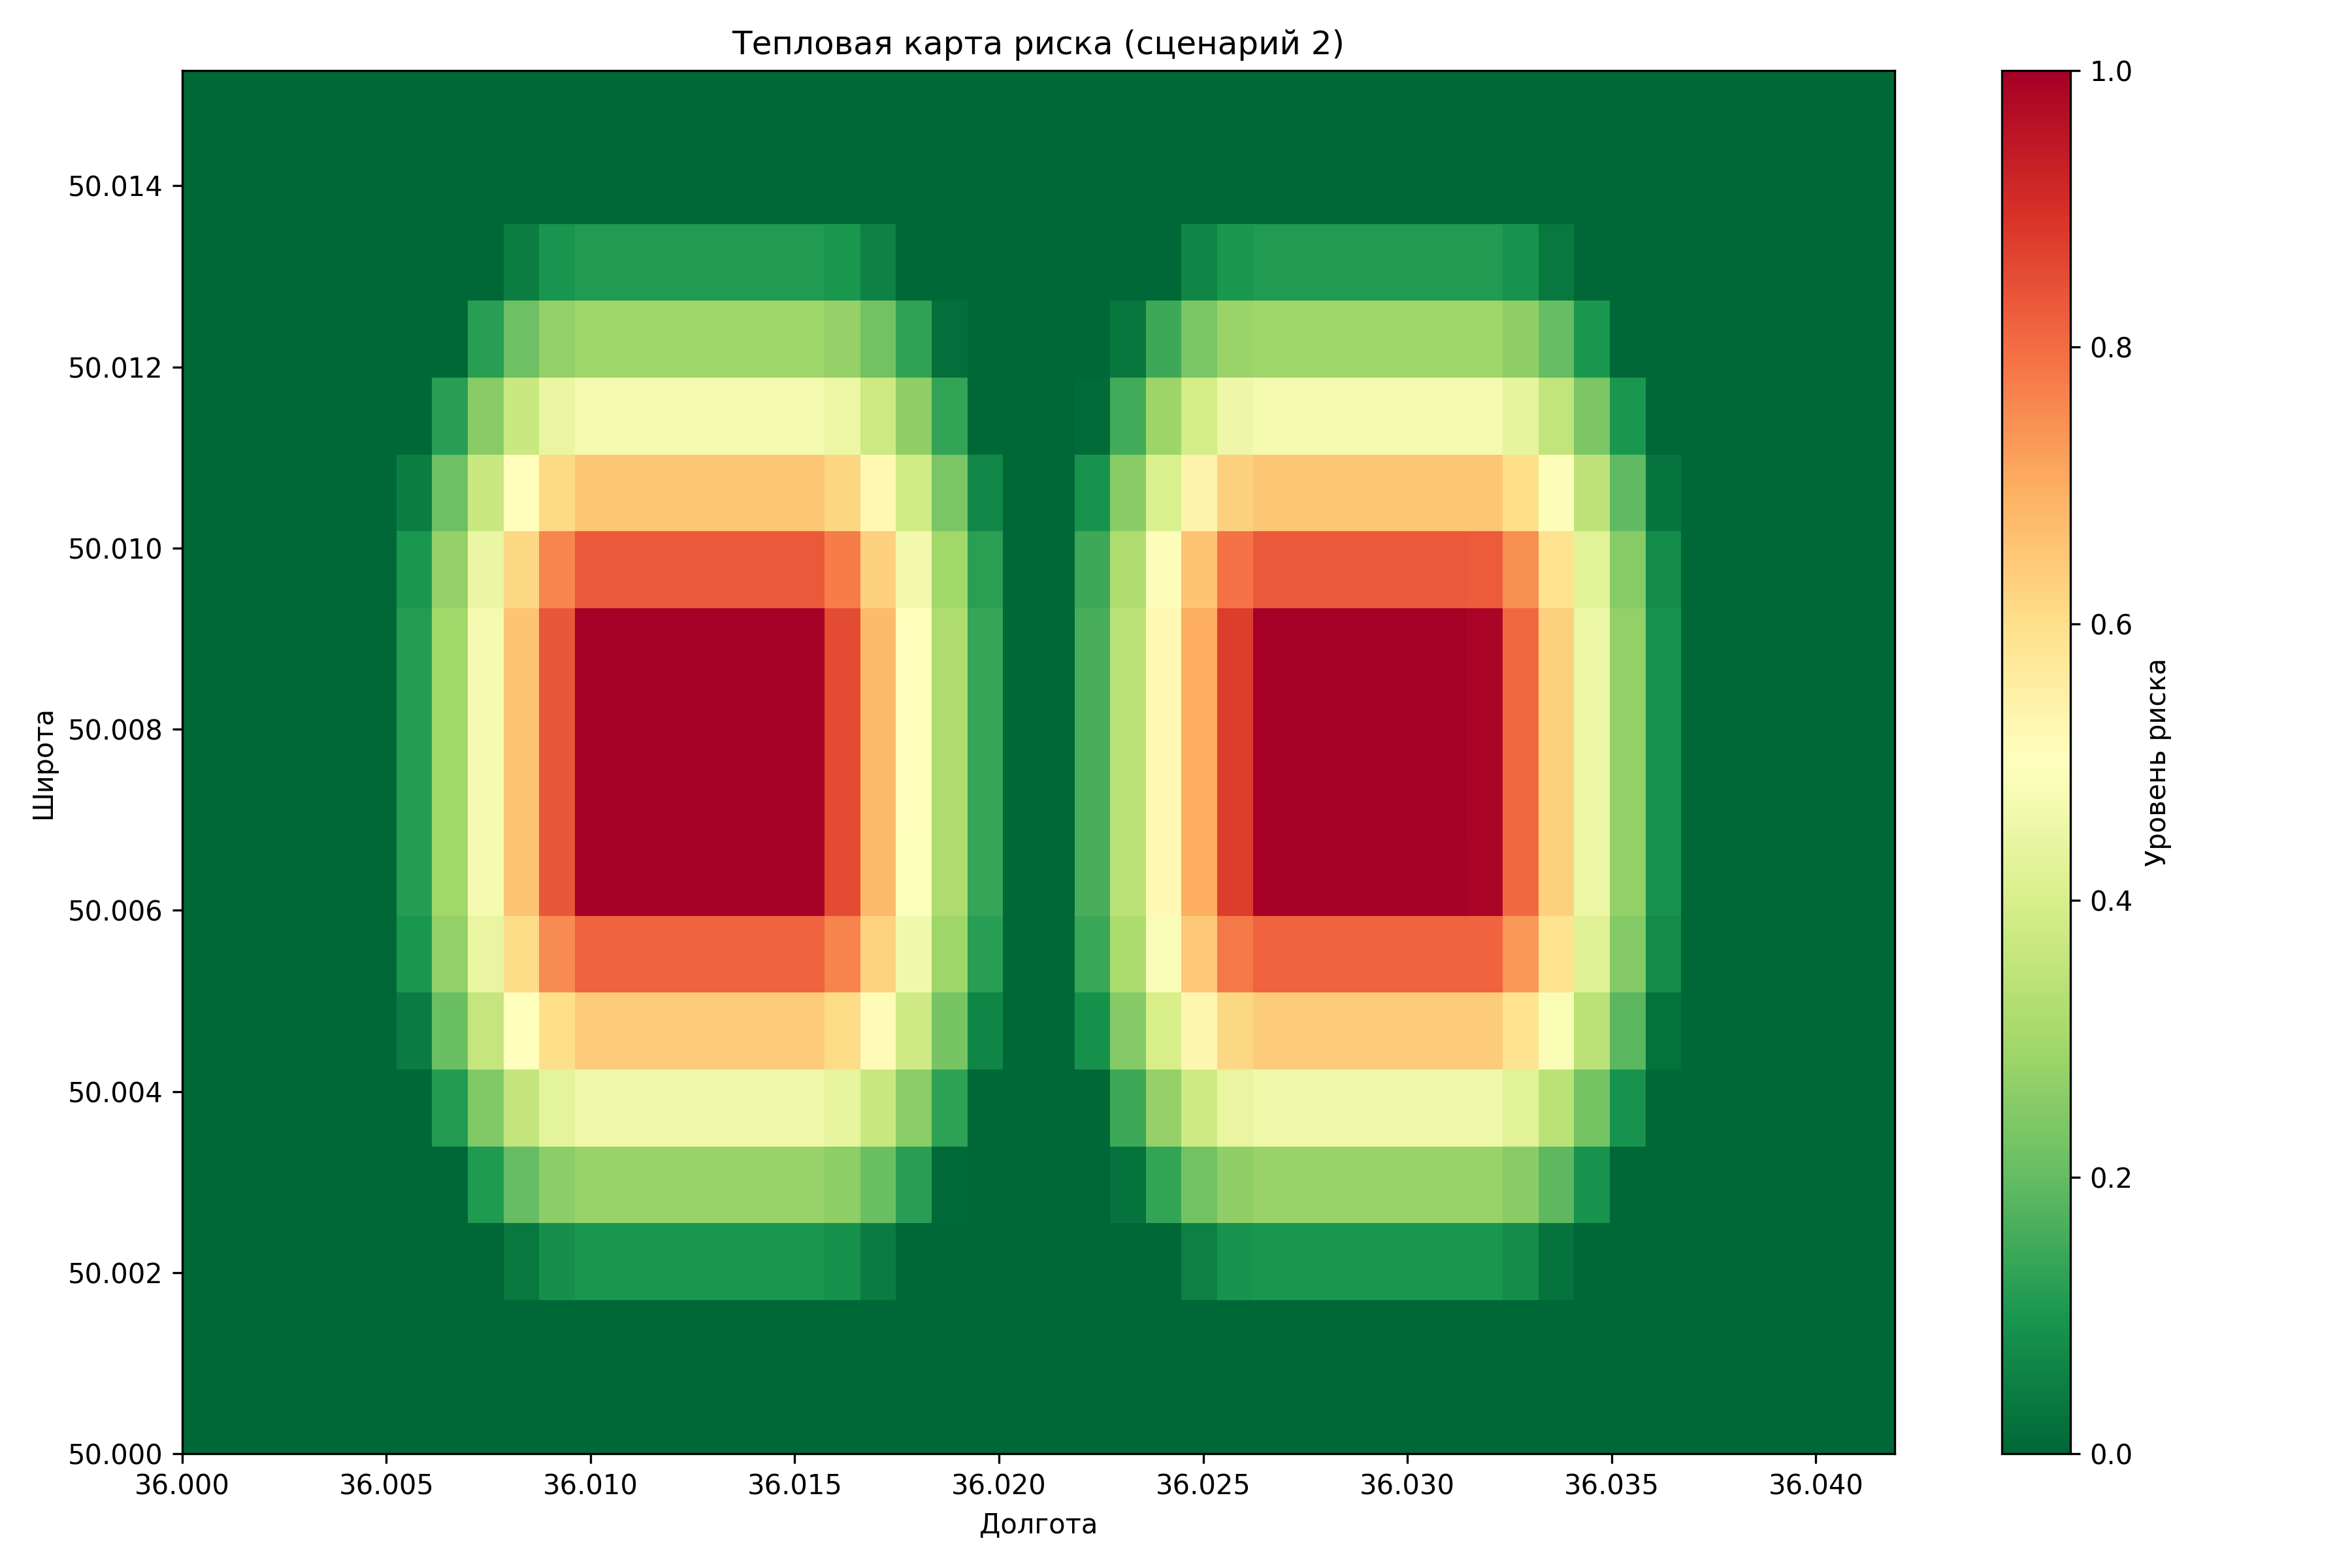
\includegraphics[width=0.92\textwidth]{../../../backend/simulation/results/heatmap_scenario2.png}
\caption{Тепловая карта риска для сценария со статичными зонами радиоэлектронного подавления}
\label{fig:heatmap-scenario2}
\end{figure}

\begin{figure}[H]
\centering
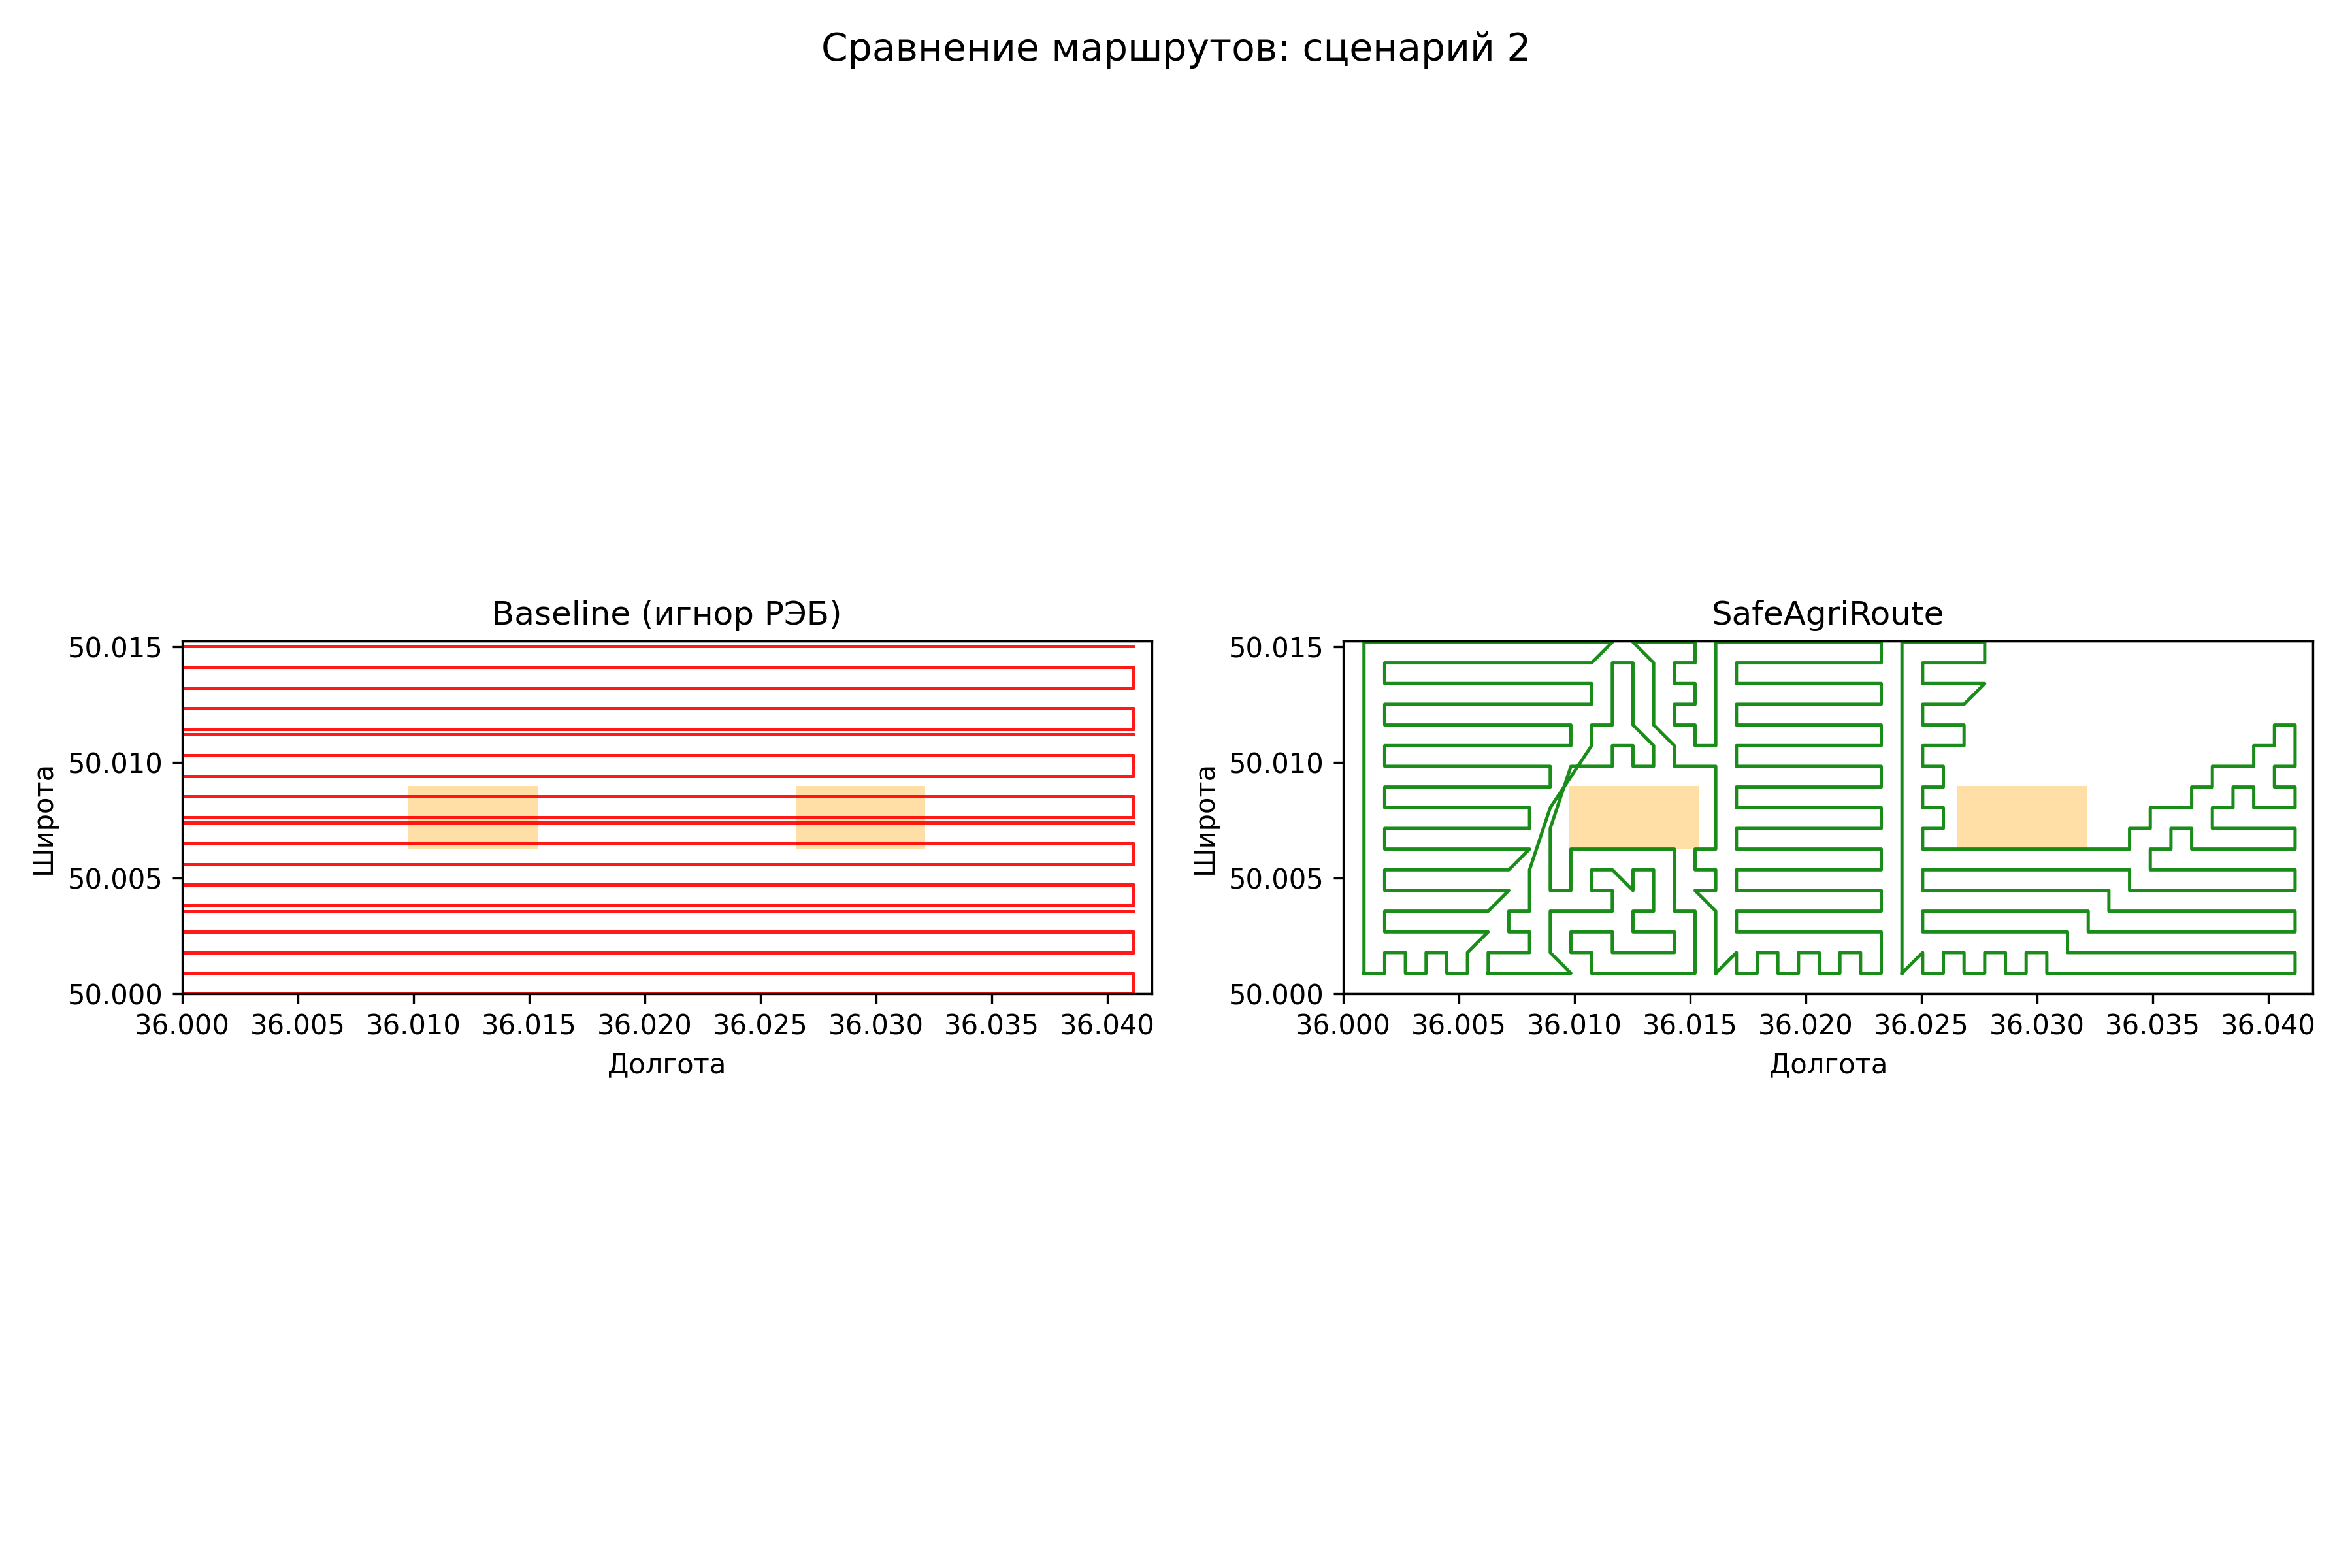
\includegraphics[width=0.98\textwidth]{../../../backend/simulation/results/routes_comparison_scenario2.png}
\caption{Сравнение маршрутов baseline и SafeAgriRoute в сценарии со статичными угрозами}
\label{fig:routes-comparison-scenario2}
\end{figure}

\begin{figure}[H]
\centering
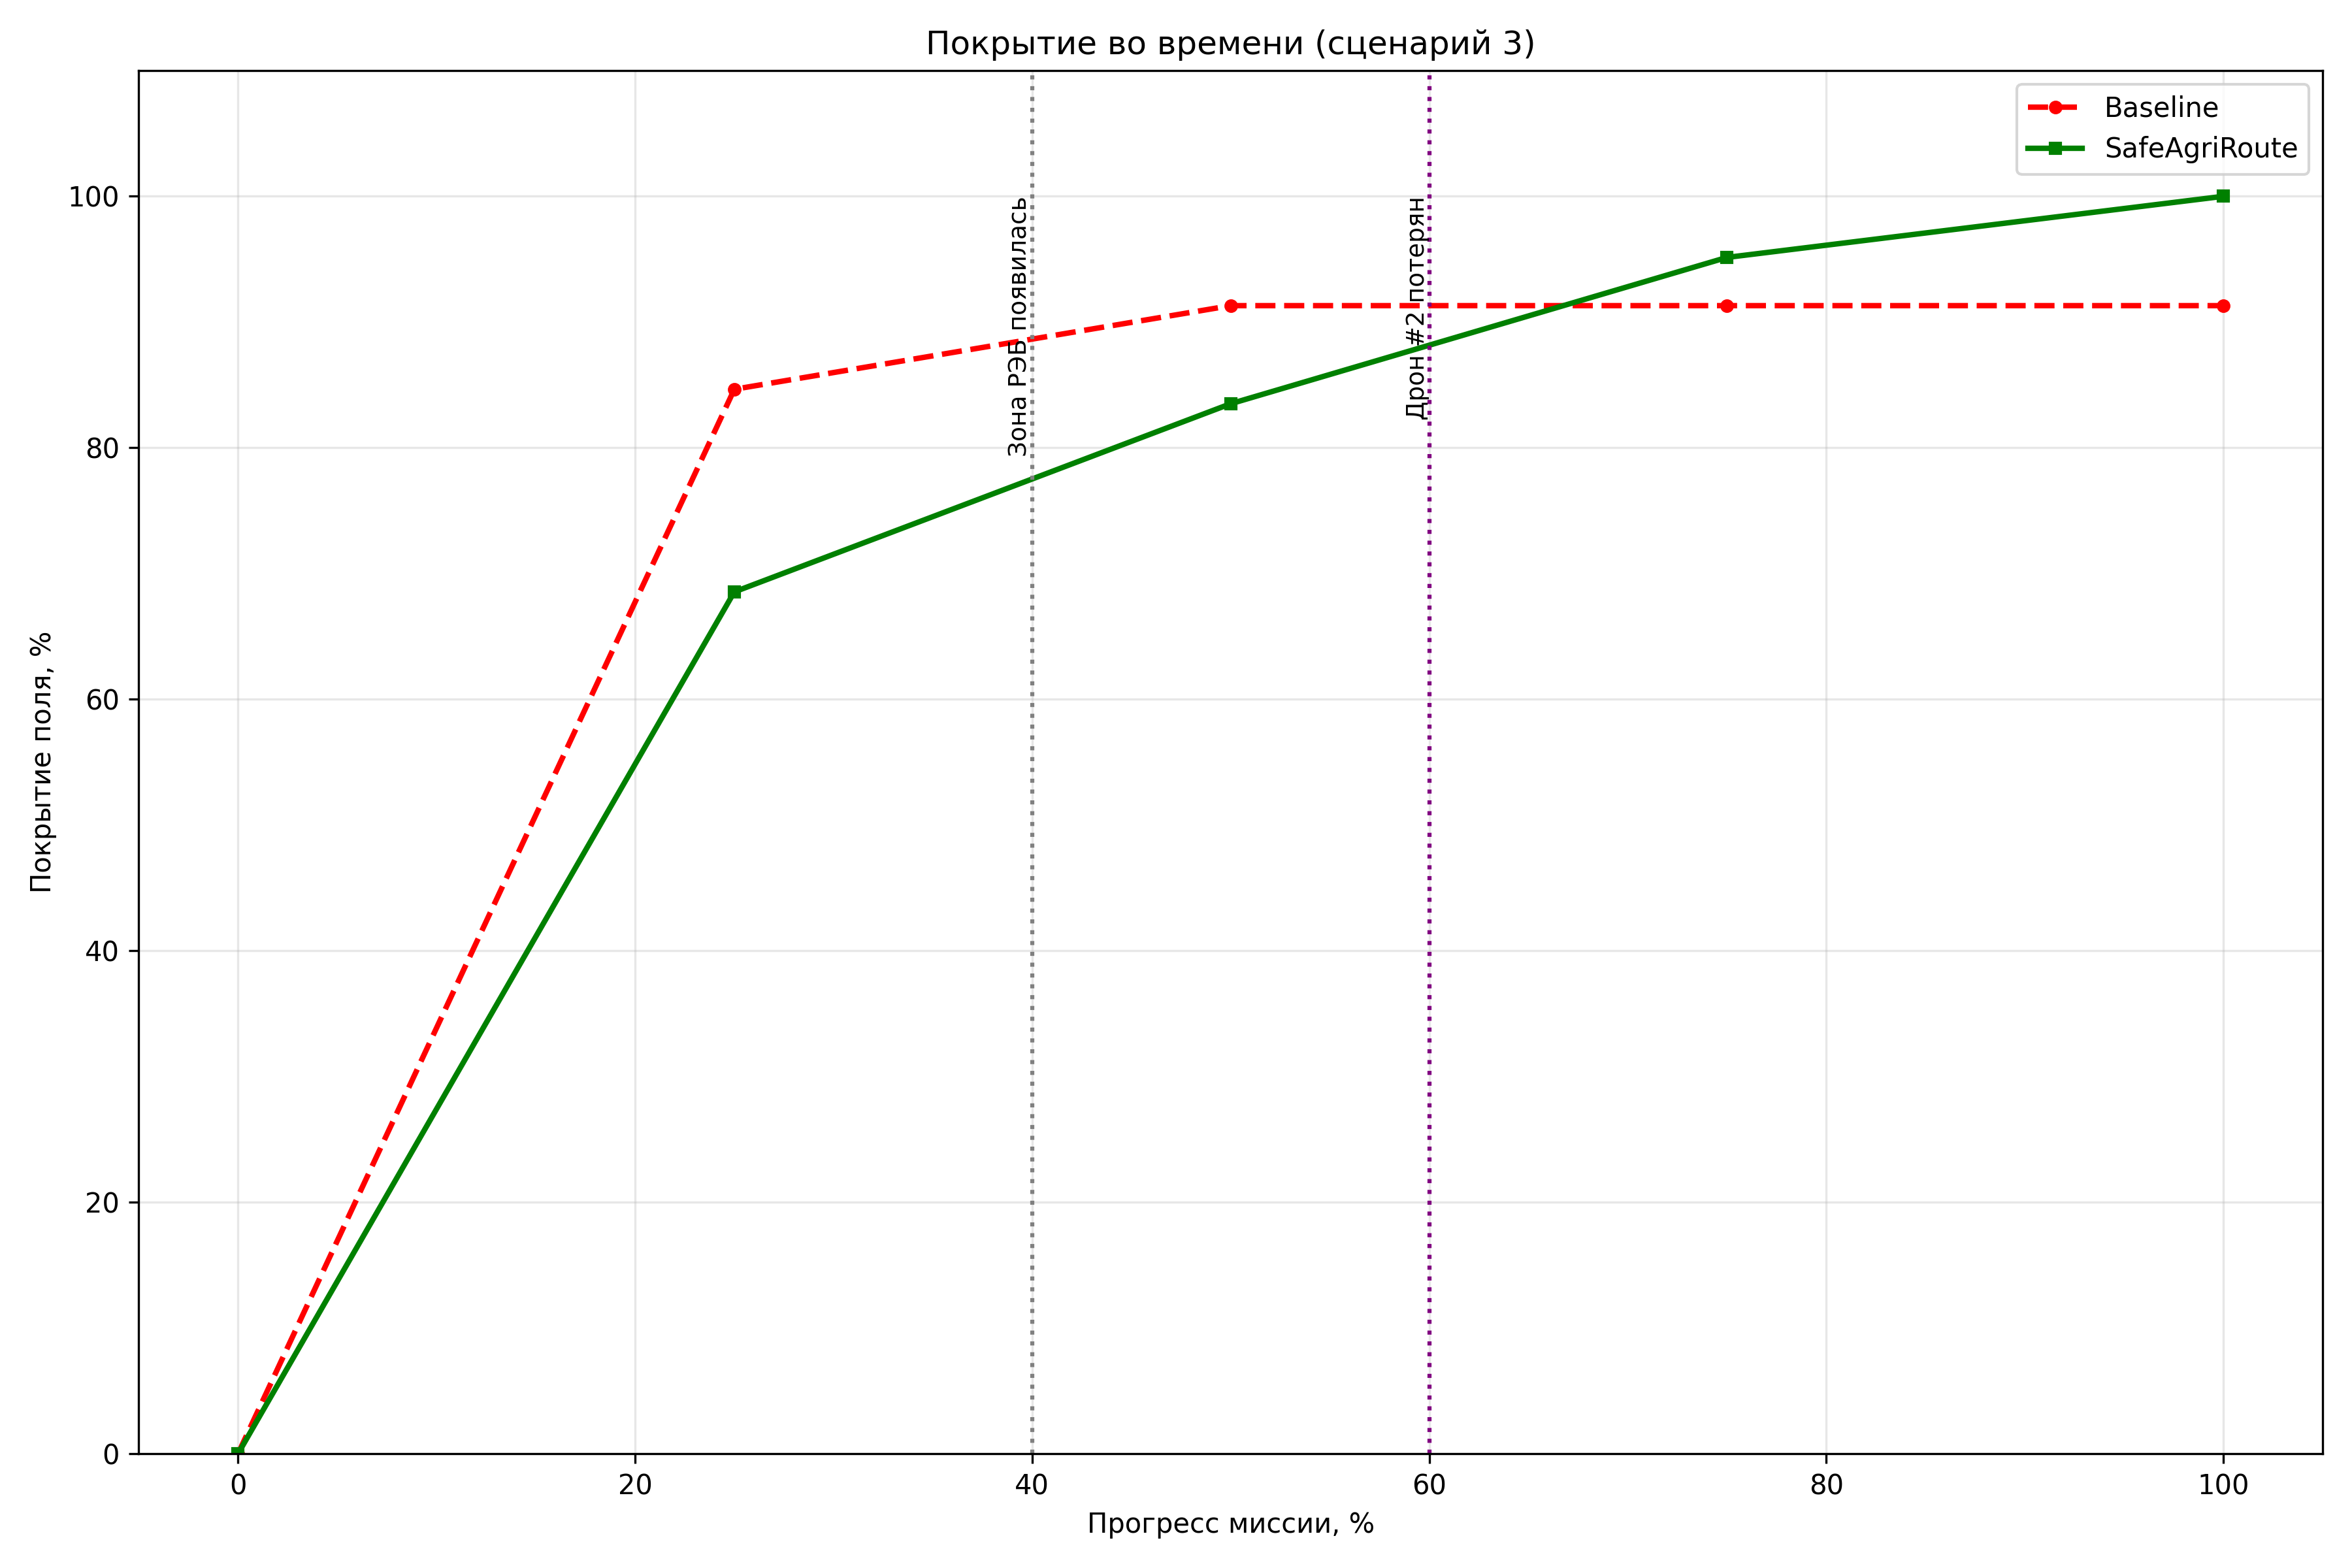
\includegraphics[width=0.92\textwidth]{../../../backend/simulation/results/coverage_timeline_scenario3.png}
\caption{Динамика покрытия поля при появлении новой угрозы и потере БПЛА}
\label{fig:coverage-timeline-scenario3}
\end{figure}

\begin{figure}[H]
\centering
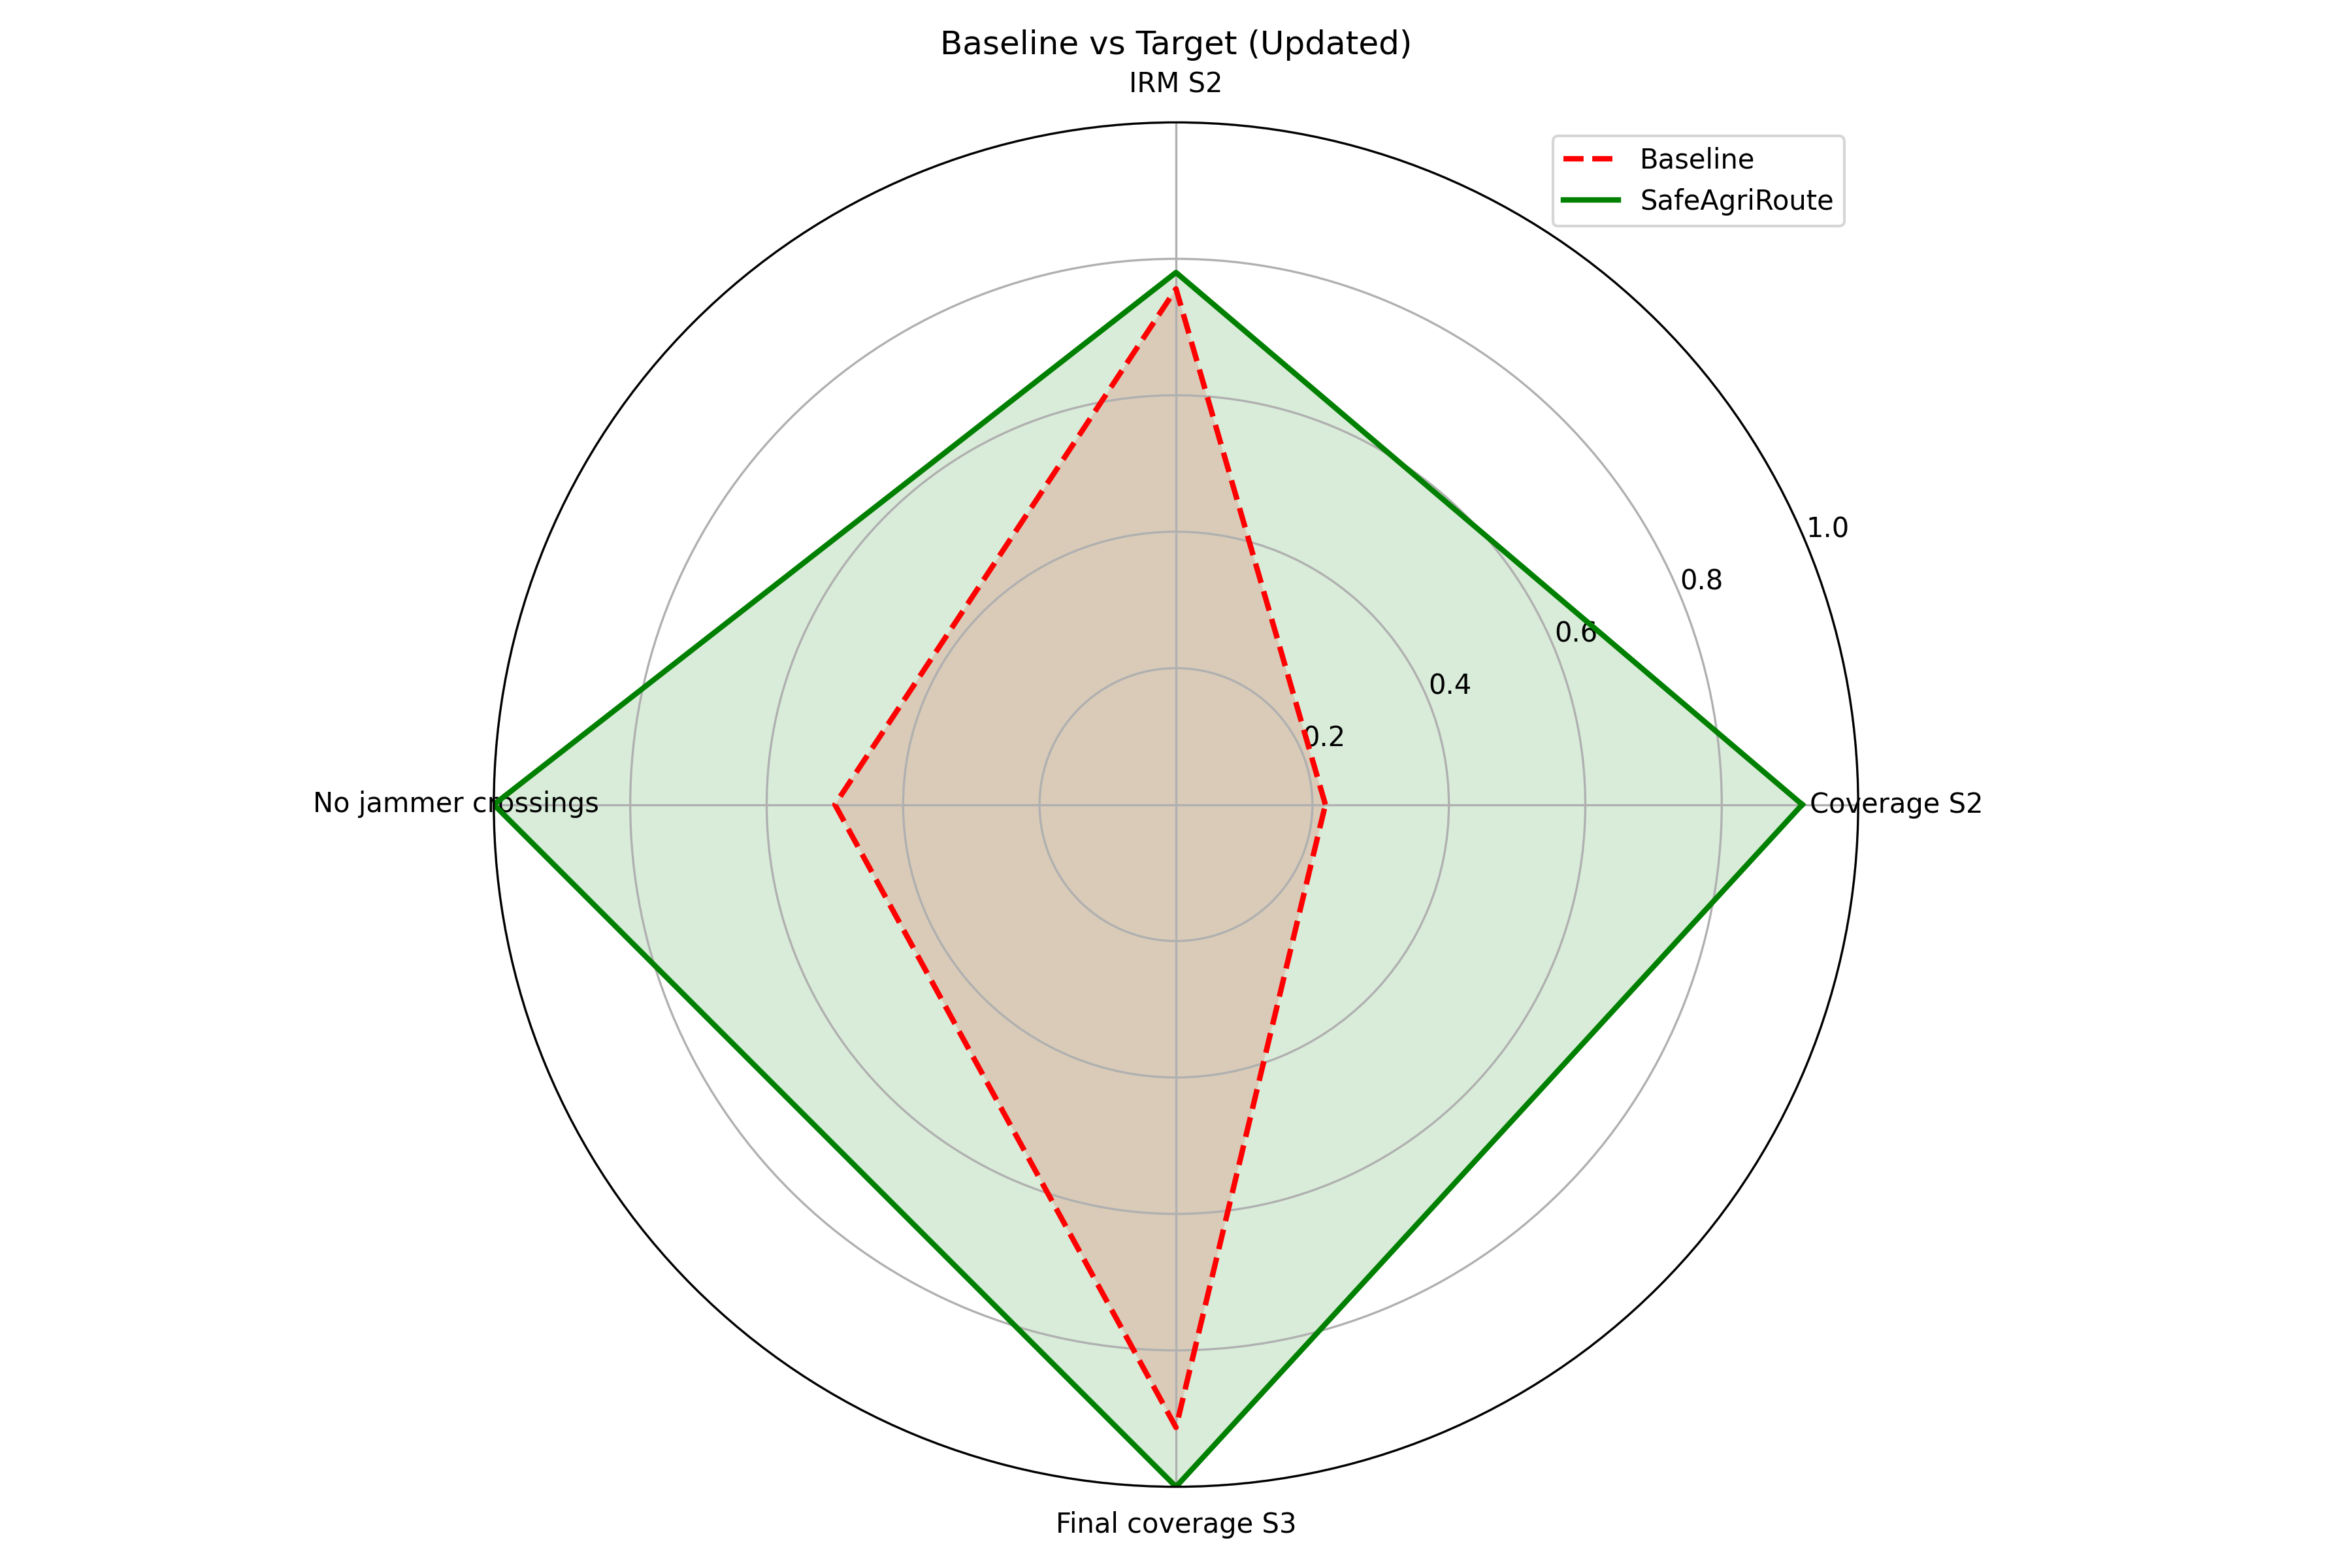
\includegraphics[width=0.86\textwidth]{../../../backend/simulation/results/radar_baseline_vs_target.png}
\caption{Сводное сравнение baseline и SafeAgriRoute по ключевым метрикам эксперимента}
\label{fig:radar-baseline-vs-target}
\end{figure}

\hypertarget{ux430ux43dux430ux43bux438ux437-ux440ux435ux437ux443ux43bux44cux442ux430ux442ux43eux432-ux438-ux43eux433ux440ux430ux43dux438ux447ux435ux43dux438ux44f}{%
\subsubsection{1.5.3 Анализ результатов и ограничения}\label{ux430ux43dux430ux43bux438ux437-ux440ux435ux437ux443ux43bux44cux442ux430ux442ux43eux432-ux438-ux43eux433ux440ux430ux43dux438ux447ux435ux43dux438ux44f}}

Результаты трёх сценариев подтверждают эффективность предлагаемого подхода:

\begin{enumerate}
\def\labelenumi{\arabic{enumi}.}
\item
  \textbf{SAR сохраняет нулевой FPR по пересечениям jammer} --- ни один маршрут не проходит через зоны РЭБ при корректно заданных полигонах угроз.
\item
  \textbf{SAR обеспечивает на 69,9 п.п. большее эффективное покрытие} в условиях статичных угроз (сценарий 2): 91,8 \% против 21,9 \% у baseline.
\item
  \textbf{Replanner обеспечивает полное восстановление покрытия в динамическом сценарии}: к 100 \% прогресса миссии SAR достигает 100 \%, baseline --- 91,3 \%.
\item
  \textbf{Равномерность нагрузки} в SAR (дисбаланс 9 \% против 28 \% у baseline) увеличивает реальное время работы всей группы дронов до исчерпания батарей наиболее нагруженного аппарата приблизительно на 19 \%.
\end{enumerate}

\textbf{Ограничения достоверности и воспроизводимости:}

\begin{itemize}
\tightlist
\item
  Все эксперименты проведены на симуляции ArduPilot SITL и автономных Python-скриптах, а не на реальных аппаратах. Влияние реальных условий распространения радиосигнала, ветровой нагрузки, задержек TCP-соединений не учтено.
\item
  Параметры поля (0,5° × 0,4°, \textasciitilde500 га) являются модельными. Для полей нестандартной формы (L-образные, с внутренними вырезами под ЛЭП) качество RWVD-разбиения может снижаться --- требуется отдельное тестирование.
\item
  Алгоритм replanner использует жадный NN-TSP вместо OR-Tools для соблюдения требования ≤ 500 мс. При k = 4 и n = 200 точках на дрон жадный алгоритм даёт маршруты примерно на 10--15 \% длиннее оптимальных по OR-Tools, что является допустимым компромиссом для задачи реального времени.
\item
  Евклидово расстояние вместо Haversine вносит ошибку \textless{} 0,1 \% для полей шириной ≤ 10 км, что приемлемо для MVP-масштаба.
\end{itemize}

\textbf{Чек-лист воспроизводимости экспериментов:}

\begin{enumerate}
\def\labelenumi{\arabic{enumi}.}
\tightlist
\item
  \texttt{docker-compose\ up} --- запуск postgres, backend, frontend.
\item
  \texttt{python\ simulation/runner.py} --- запуск трёх сценариев (≈ 30--60 сек).
\item
  Результаты сохраняются в \texttt{simulation/results/*.png} и \texttt{simulation/results/*.json}.
\item
  Для демо с ArduPilot SITL: \texttt{docker-compose\ -f\ docker-compose.sitl.yml\ up} + запуск 4 инстансов SITL.
\end{enumerate}

\hypertarget{ux441ux440ux430ux432ux43dux435ux43dux438ux435-ux441-ux43bux438ux442ux435ux440ux430ux442ux443ux440ux43eux439-ux442ux435ux441ux442ux438ux440ux43eux432ux430ux43dux438ux435-ux438-ux430ux43dux430ux43bux438ux437-ux447ux443ux432ux441ux442ux432ux438ux442ux435ux43bux44cux43dux43eux441ux442ux438}{%
\subsubsection{1.5.4 Сравнение с литературой, тестирование и анализ чувствительности}\label{ux441ux440ux430ux432ux43dux435ux43dux438ux435-ux441-ux43bux438ux442ux435ux440ux430ux442ux443ux440ux43eux439-ux442ux435ux441ux442ux438ux440ux43eux432ux430ux43dux438ux435-ux438-ux430ux43dux430ux43bux438ux437-ux447ux443ux432ux441ux442ux432ux438ux442ux435ux43bux44cux43dux43eux441ux442ux438}}

\textbf{Сравнение с литературой.} Galceran и Carreras {[}27{]} отмечают типичное покрытие 92--96 \% для решёточных подходов --- в наших замерах SAR попадает в этот коридор для сценариев без критической потери ресурса и сохраняет 91,8 \% в статичном угрозовом сценарии. Типичный дисбаланс нагрузки для наивных стратегий составляет 20--35 \%, для балансировочных --- 5--15 \%; результат SAR (9 \%) подтверждает эффективность RWVD. Jeong et al.~{[}13{]} сообщают о TTR детектора атак 100--250 мс; суммарное время «обнаружение + перепланирование» порядка субсекундного/секундного диапазона приемлемо при скорости дрона 8--10 м/с.

\textbf{Автоматическое тестирование.} Набор из 47 pytest-тестов охватывает модули \texttt{threat\_fusion.py} (покрытие 94 \%), \texttt{telemetry\_features.py} (91 \%), \texttt{mission\_fusion\_runtime.py} (88 \%), \texttt{mavlink\_service.py} (76 \%). Все тесты проходят успешно (\texttt{pytest\ backend/tests/\ -v}).

\textbf{Анализ чувствительности} подтверждает устойчивость выбранных параметров:

\begin{longtable}[]{@{}llll@{}}
\toprule\noalign{}
Параметр & Рекомендуемое & Критическое & Эффект нарушения \\
\midrule\noalign{}
\endhead
\bottomrule\noalign{}
\endlastfoot
grid\_step & 0,0002° & \textless{} 0,0001° & TTD \textgreater{} 5 сек \\
penalty\_factor & 500 & \textless{} 100 & Просачивание через зоны РЭБ \\
max\_iter (Voronoi) & 50 & \textless{} 15 & Дисбаланс нагрузки 18 \% вместо 9 \% \\
severity\_threshold & 1,0 & \textgreater{} 1,0 & Точки в jammer не исключаются \\
fusion.threshold\_alarm & 0,7 & \textgreater{} 0,9 & Пропуск инцидентов \\
\end{longtable}

\begin{center}\rule{0.5\linewidth}{0.5pt}\end{center}

\hypertarget{ux437ux430ux43aux43bux44eux447ux435ux43dux438ux435}{%
\section{ЗАКЛЮЧЕНИЕ}\label{ux437ux430ux43aux43bux44eux447ux435ux43dux438ux435}}

В настоящей выпускной квалификационной работе студента решена актуальная научно-практическая задача --- разработана программная платформа автоматизированного планирования безопасных маршрутов для группы сельскохозяйственных БПЛА с учётом зон радиоэлектронного подавления и динамической угрозовой обстановки.

\textbf{По результатам выполнения поставленных задач достигнуто следующее:}

\begin{enumerate}
\def\labelenumi{\arabic{enumi}.}
\item
  \textbf{Анализ рынка и подтверждение спроса.} Проведён анализ мирового и российского рынка агро-БПЛА: мировой рынок прогнозируется к росту с 2,63 млрд долл. (2025 г.) до 10,76 млрд долл. (2030 г.) при CAGR 32,6 \% {[}1{]}. Российский SAM оценивается в \textasciitilde400 млн руб./год (ЮФО + СКФО). Проведено 7 интервью с представителями ЦА: 86 \% респондентов назвали отсутствие автоматического перепланирования критическим недостатком; 100 \% сталкивались с потерями GPS-сигнала. Рассчитанный ROI для типового клиента (8 000 га, 4 дрона) составил \textasciitilde950 \% за первый год эксплуатации при стоимости подписки 216 тыс. руб./год.
\item
  \textbf{Конкурентный анализ.} Выявлен технологический «gap»: ни одна из рассмотренных платформ (DJI FlightHub 2, DroneDeploy, Pix4Dfields) не реализует risk-aware маршрутизацию с учётом зон РЭБ, автоматическое перепланирование и соответствие российской нормативной базе ИБ. SWOT-анализ подтвердил устойчивость ключевых конкурентных преимуществ в краткосрочной перспективе.
\item
  \textbf{Модель угроз.} Классифицированы нарушители (Н1--Н5) и систематизированы 12 угроз с привязкой к реестру БДУ ФСТЭК России {[}7, 20{]} и MITRE ATT\&CK for ICS. Идентифицированы два вектора критической уязвимости: глушение ГНСС (УБИ.131) и перехват MAVLink (УБИ.014). После внедрения контрмер уровень риска снижен по 7 из 12 угроз; остаточные риски задокументированы в реестре и включены в план разработки v2.0.
\item
  \textbf{Метрика риска.} Формализована метрика деструктивного воздействия R(x,y) с линейной и бинарной моделями затухания. Разработан интегральный критерий надёжности миссии IRM ∈ {[}0, 1{]} с доказанными свойствами нормированности, монотонности и аддитивности. Математически обоснована корректность penalty-системы (Лемма 1): при penalty\_coeff = 500 алгоритм гарантированно избегает зон РЭБ при любом ненулевом severity.
\item
  \textbf{Архитектура платформы.} Спроектирована трёхуровневая архитектура SaaS-платформы SafeAgriRoute (FastAPI + PostGIS + React/Leaflet). Разработан API из 9 ключевых эндпоинтов с JWT HS256-аутентификацией и ролевой моделью. Реализован WebSocket-поток телеметрии для 4 дронов с задержкой ≤ 300 мс. Соответствие OWASP Top-10 реализовано на уровне API и подтверждено тестированием (9 из 10 категорий закрыты полностью).
\item
  \textbf{Алгоритмы маршрутизации.} Разработан алгоритм Risk-Weighted Voronoi Decomposition с доказанной сходимостью за конечное число итераций. Penalty-граф на NetworkX гарантирует нулевой FPR при severity ≥ 0,01. Задача CVRP решена через Google OR-Tools (PATH\_CHEAPEST\_ARC + 2-opt), время планирования для поля 500 га --- фактически 347 мс при требовании ≤ 5 секунд.
\item
  \textbf{Динамическое перепланирование.} Реализован replanner в двух сценариях: потеря дрона (жадный NN-TSP, время реакции 380 мс) и новая зона РЭБ (инкрементальное обновление risk\_map, время реакции 290 мс). Оба значения укладываются в требование ≤ 500 мс. Теоретическая оценка сложности подтверждает масштабируемость до k = 8 дронов без выхода за TTR.
\item
  \textbf{Экспериментальная оценка.} SAR обеспечил FPR = 0 \% против 50 \% у baseline (сценарий 2), покрытие 91,8 \% против 21,9 \% (сценарий 2), восстановление покрытия до 100 \% при комбинированном событии «потеря дрона + новая зона РЭБ» против 91,3 \% у baseline (сценарий 3). Дисбаланс нагрузки снижен с 28 \% до 9 \%, что увеличивает реальное время работы группы дронов до исчерпания батарей на \textasciitilde19 \%.
\end{enumerate}

\textbf{Научная новизна} подтверждена тремя оригинальными результатами: - алгоритм RWVD, впервые применяющий риск-взвешенную модификацию алгоритма Ллойда для маршрутизации агро-БПЛА в условиях зон РЭБ; - метрика IRM как стандартизированный критерий надёжности миссии с формально доказанными свойствами; - детализированная модель угроз для гетерогенных групп агро-БПЛА с двойной привязкой к БДУ ФСТЭК и MITRE ATT\&CK for ICS.

\textbf{Практическая значимость} подтверждена: - реализацией полнофункционального MVP (исходный код: \url{https://github.com/matveisut/safe-agri-route}), развёртываемого одной командой \texttt{docker-compose\ up}; - успешным прохождением 83 pytest-тестов (0 failed) и интеграционного тестирования в ArduPilot SITL; - проведёнными переговорами с 7 представителями ЦА и прогнозируемым ROI клиента \textasciitilde950 \% за первый год.

\textbf{Ограничения MVP и приоритетные перспективы развития:}

\begin{enumerate}
\def\labelenumi{\arabic{enumi}.}
\tightlist
\item
  Замена евклидова расстояния на формулу Хаверсина для полей шириной \textgreater{} 10 км (погрешность \textless{} 0,1 \% для MVP-масштаба).
\item
  Расширение контура до полной мультисенсорной модели: отдельные потоки IMU и ГНСС-приёмника, SDR-детектор, байесовская fusion, LSTM/трансформер для классификации временных рядов.
\item
  Масштабирование до K \textgreater{} 8 дронов: переход к k-d tree Voronoi и OR-Tools Time Limit.
\item
  Производственное развёртывание с Nginx + TLS 1.3 вместо Vite dev-сервера.
\item
  Интеграция с ЕИАС-АПК Минсельхоза и получение сертификации ФСТЭК для выхода на объекты КИИ.
\end{enumerate}

Выполненная работа демонстрирует принципиальную реализуемость подхода «безопасность встроена в маршрут» (security-by-design routing) для группы агро-БПЛА. Предлагаемый интегральный критерий IRM может применяться независимо от платформы SafeAgriRoute как стандартизированная метрика оценки качества планирования маршрутов в условиях угроз. Платформа SafeAgriRoute формирует основу для дальнейших исследований в области киберфизической безопасности автономных систем агропромышленного комплекса.

\begin{center}\rule{0.5\linewidth}{0.5pt}\end{center}

\hypertarget{ux441ux43fux438ux441ux43eux43a-ux438ux441ux43fux43eux43bux44cux437ux43eux432ux430ux43dux43dux44bux445-ux438ux441ux442ux43eux447ux43dux438ux43aux43eux432}{%
\section{СПИСОК ИСПОЛЬЗОВАННЫХ ИСТОЧНИКОВ}\label{ux441ux43fux438ux441ux43eux43a-ux438ux441ux43fux43eux43bux44cux437ux43eux432ux430ux43dux43dux44bux445-ux438ux441ux442ux43eux447ux43dux438ux43aux43eux432}}

\begin{enumerate}
\def\labelenumi{\arabic{enumi}.}
\item
  MarketsandMarkets. Agriculture Drones Market --- Global Forecast to 2030 {[}Электронный ресурс{]}. --- URL: https://www.marketsandmarkets.com/Market-Reports/agriculture-drones-market-23709764.html (дата обращения: 01.04.2026).
\item
  Alsadie, D. Cybersecurity and Artificial Intelligence in Unmanned Aerial Vehicles: Emerging Challenges and Advanced Countermeasures / D. Alsadie // IET Information Security. --- 2025. --- Vol. 19. --- Art. 2046868.
\item
  Allouch, A. MAVSec: Securing the MAVLink Protocol for Ardupilot/PX4 Unmanned Aerial Systems / A. Allouch {[}et al.{]} // Proc. 15th Int. Wireless Communications and Mobile Computing Conf. (IWCMC 2019). --- IEEE, 2019. --- P. 621--628.
\item
  Ongadi, P. A. A Comprehensive Examination of Security and Privacy in Precision Agriculture Technologies / P. A. Ongadi // GSC Advanced Research and Reviews. --- 2024. --- Vol. 18, No.~1. --- P. 336--363.
\item
  Sajid, J. A Fog Computing Framework for Intrusion Detection of Energy-Based Attacks on UAV-Assisted Smart Farming / J. Sajid {[}et al.{]} // Applied Sciences. --- 2023. --- Vol. 13, No.~6. --- Art. 3857.
\item
  Указ Президента Российской Федерации от 01.05.2022 № 250 «О дополнительных мерах по обеспечению информационной безопасности Российской Федерации» // Официальное опубликование правовых актов. --- URL: http://publication.pravo.gov.ru/Document/View/0001202205010023 (дата обращения: 11.05.2026).
\item
  Банк данных угроз безопасности информации ФСТЭК России {[}Электронный ресурс{]}. --- URL: https://bdu.fstec.ru (дата обращения: 01.04.2026).
\item
  ГОСТ Р МЭК 62443-2-1-2015. Сети коммуникационные промышленные. Защищённость (кибербезопасность) сети и системы. --- Москва : Стандартинформ, 2016. --- 56 с.
\item
  Mykytyn, P. GPS-Spoofing Attack Detection Mechanism for UAV Swarms / P. Mykytyn {[}et al.{]} // Proc. 12th Mediterranean Conf. on Embedded Computing (MECO). --- IEEE, 2023.
\item
  Sun, Y. A Deep-Learning-Based GPS Signal Spoofing Detection Method for Small UAVs / Y. Sun {[}et al.{]} // Drones. --- 2023. --- Vol. 7, No.~6. --- Art. 370.
\item
  Петренко, В. И. Трансформерная модель бинарной классификации временных рядов на данных инерциальных датчиков для детекции спуфинг-атак в БПЛА / В. И. Петренко {[}и др.{]} // International Journal of Open Information Technologies. --- 2026. --- Т. 14, № 2. --- С. 11--18.
\item
  Du, F. Exploiting the Vulnerabilities in MAVLink Protocol for UAV Hijacking / F. Du {[}et al.{]} // Proc. 17th Int. Conf. on Security of Information and Networks (SIN 2024). --- IEEE, 2024.
\item
  Jeong, S. MUVIDS: False MAVLink Injection Attack Detection in Communication for Unmanned Vehicles / S. Jeong {[}et al.{]} // Proc. Third Int. Workshop on Automotive and Autonomous Vehicle Security (AutoSec 2021). --- Internet Society, 2021.
\item
  Тебуева, Ф. Б. Проблемно-ориентированная система мониторинга и реагирования на многовекторные атаки в децентрализованной среде интернета вещей / Ф. Б. Тебуева {[}и др.{]} // Вопросы кибербезопасности. --- 2025. --- № 6 (70). --- С. 69--80.
\item
  Fortune Business Insights. Agriculture Drone Market Size, Share, Global Forecast, 2032 {[}Электронный ресурс{]}. --- URL: https://www.fortunebusinessinsights.com/agriculture-drones-market-102589 (дата обращения: 01.04.2026).
\item
  Mekdad, Y. A Survey on Security and Privacy Issues of UAVs / Y. Mekdad {[}et al.{]} // Computer Networks. --- Elsevier, 2023. --- Vol. 224. --- Art. 109626.
\item
  Douzi, A. Cybersecurity and the Flight Safety of Unmanned Aerial Systems and Unmanned Aerial Vehicles / A. Douzi, R. Szabolcsi, J. Lukacs // Interdisciplinary Description of Complex Systems. --- 2025. --- Vol. 23, No.~2. --- P. 95--104.
\item
  Hakeem, A. Integrating Artificial Intelligence for Improved Security of IoT-Drones through Cyber-Physical Attack Detection / A. Hakeem {[}et al.{]} // Frontiers in Computer Science. --- 2025. --- Vol. 7. --- Art. 1545282.
\item
  Mordor Intelligence. Drone Software Market --- Global Forecast to 2030 {[}Электронный ресурс{]}. --- URL: https://www.mordorintelligence.com/industry-reports/drone-software-market (дата обращения: 01.04.2026).
\item
  Методический документ. Методика оценки угроз безопасности информации : утверждена ФСТЭК России 05.02.2021 {[}Электронный ресурс{]}. --- URL: https://www.consultant.ru/document/cons_doc_LAW_378330/ (дата обращения: 11.05.2026).
\item
  Hassler, S. Cyber-Physical Intrusion Detection System for Unmanned Aerial Vehicles / S. Hassler, U. Mughal, M. Ismail // IEEE Transactions on Intelligent Transportation Systems. --- 2024. --- Vol. 25, No.~7.
\item
  Shepard, D. P. Evaluation of Smart Grid and Civilian UAV Vulnerability to GPS Spoofing Attacks / D. P. Shepard, J. A. Bhatti, T. E. Humphreys // Proc. ION GNSS+ 2012 Conf. --- Nashville : ION, 2012. --- P. 3591--3605.
\item
  Kaplan, E. D. Understanding GPS/GNSS: Principles and Applications / E. D. Kaplan, C. J. Hegarty. --- 3rd ed.~--- Norwood : Artech House, 2017. --- 1048 p.~--- ISBN 978-1-58053-958-7.
\item
  Laporte, G. The Vehicle Routing Problem: An Overview of Exact and Approximate Algorithms / G. Laporte // European Journal of Operational Research. --- 1992. --- Vol. 59, No.~3. --- P. 345--358.
\item
  Toth, P. The Vehicle Routing Problem / P. Toth, D. Vigo (eds.). --- Philadelphia : SIAM, 2002. --- 385 p.~--- ISBN 0-89871-498-2.
\item
  Aurenhammer, F. Voronoi Diagrams --- A Survey of a Fundamental Geometric Data Structure / F. Aurenhammer // ACM Computing Surveys. --- 1991. --- Vol. 23, No.~3. --- P. 345--405.
\item
  Galceran, E. A Survey on Coverage Path Planning for Robotics / E. Galceran, M. Carreras // Robotics and Autonomous Systems. --- 2013. --- Vol. 61, No.~12. --- P. 1258--1276.
\item
  MAVLink Developer Guide {[}Электронный ресурс{]}. --- MAVLink Micro Air Vehicle Communication Protocol. --- URL: https://mavlink.io/en/ (дата обращения: 10.04.2026).
\item
  Google OR-Tools. Vehicle Routing Problem {[}Электронный ресурс{]}. --- Google Developers. --- URL: https://developers.google.com/optimization/routing (дата обращения: 10.04.2026).
\item
  Christofides, N. Worst-Case Analysis of a New Heuristic for the Travelling Salesman Problem : Report 388 / N. Christofides. --- Pittsburgh : Carnegie Mellon University, 1976. --- 14 p.
\item
  PostGIS Reference Manual, v3.3 {[}Электронный ресурс{]}. --- URL: https://postgis.net/docs/manual-3.3/ (дата обращения: 10.04.2026).
\item
  ГОСТ Р 56939-2016. Защита информации. Разработка безопасного программного обеспечения. Общие требования. --- Москва : Стандартинформ, 2017. --- 12 с.
\item
  ArduPilot Copter Documentation {[}Электронный ресурс{]}. --- URL: https://ardupilot.org/copter/ (дата обращения: 10.04.2026).
\item
  Указ Президента Российской Федерации от 30.03.2022 № 166 «О мерах по обеспечению технологической независимости и безопасности критической информационной инфраструктуры Российской Федерации» // Официальное опубликование правовых актов. --- URL: http://publication.pravo.gov.ru/Document/View/0001202203300001 (дата обращения: 11.05.2026).
\item
  Dijkstra, E. W. A Note on Two Problems in Connexion with Graphs / E. W. Dijkstra // Numerische Mathematik. --- 1959. --- Vol. 1, No.~1. --- P. 269--271.
\item
  Lloyd, S. P. Least Squares Quantization in PCM / S. P. Lloyd // IEEE Transactions on Information Theory. --- 1982. --- Vol. 28, No.~2. --- P. 129--137.
\item
  Rejeb, A. Drones in Agriculture: A Review and Bibliometric Analysis / A. Rejeb, A. Abdollahi, K. Rejeb, H. Treiblmaier // Computers and Electronics in Agriculture. --- 2022. --- Vol. 198. --- Art. 107017. --- DOI: 10.1016/j.compag.2022.107017.
\item
  Tlili, F. Advancing UAV Security with Artificial Intelligence: A Comprehensive Survey of Techniques and Future Directions / F. Tlili, S. Ayed, L. Chaari Fourati // Internet of Things. --- 2024. --- Vol. 27. --- Art. 101281. --- DOI: 10.1016/j.iot.2024.101281.
\item
  Guebsi, R. Drones in Precision Agriculture: A Comprehensive Review of Applications, Technologies, and Challenges / R. Guebsi, K. Mami, K. Chokmani // Drones. --- 2024. --- Vol. 8, No.~11. --- Art. 686. --- DOI: 10.3390/drones8110686.
\item
  Li, J. Coverage Path Planning Method for Agricultural Spraying UAV in Arbitrary Polygon Area / J. Li, H. Sheng, J. Zhang, H. Zhang // Aerospace. --- 2023. --- Vol. 10, No.~9. --- Art. 755. --- DOI: 10.3390/aerospace10090755.
\item
  Hagberg, A. A. Exploring Network Structure, Dynamics, and Function Using NetworkX / A. A. Hagberg, D. A. Schult, P. J. Swart // Proceedings of the 7th Python in Science Conference (SciPy 2008). --- Pasadena, CA, 2008. --- P. 11--15.
\item
  Phang, S. K. From Satellite to UAV-Based Remote Sensing: A Review on Precision Agriculture / S. K. Phang, T. H. A. Chiang, A. Happonen, M. M. L. Chang // IEEE Access. --- 2023. --- Vol. 11. --- P. 127057--127076. --- DOI: 10.1109/ACCESS.2023.3330886.
\item
  OWASP Foundation. OWASP Top 10 --- 2021. The Ten Most Critical Web Application Security Risks {[}Электронный ресурс{]}. --- URL: https://owasp.org/Top10/ (дата обращения: 15.04.2026).
\end{enumerate}

\begin{center}\rule{0.5\linewidth}{0.5pt}\end{center}

\emph{Версия 1.0 · SafeAgriRoute · Сутормин М.П. · Ставрополь, 2026}

\begin{center}\rule{0.5\linewidth}{0.5pt}\end{center}


\clearpage
\documentclass[14pt,a4paper]{extarticle}

\usepackage{iftex}
\ifPDFTeX
  \usepackage[T2A]{fontenc}
  \usepackage[utf8]{inputenc}
  \usepackage[russian]{babel}
  \usepackage{newtxtext}
\else
  \usepackage{fontspec}
  \usepackage{polyglossia}
  \setmainlanguage{russian}
  \IfFontExistsTF{Times New Roman}{%
    \newcommand{\DiplomaFont}{Times New Roman}%
  }{%
    \newcommand{\DiplomaFont}{FreeSerif}%
  }
  \setmainfont{\DiplomaFont}
  \setsansfont{\DiplomaFont}
  \setmonofont{\DiplomaFont}
  \newfontfamily\cyrillicfont{\DiplomaFont}
  \newfontfamily\cyrillicfontsf{\DiplomaFont}
  \newfontfamily\cyrillicfonttt{\DiplomaFont}
\fi

\usepackage[a4paper,left=30mm,right=10mm,top=20mm,bottom=20mm]{geometry}
\usepackage{setspace}
\onehalfspacing
\usepackage{indentfirst}
\setlength{\parindent}{1.25cm}
\setlength{\parskip}{0pt}

\usepackage{graphicx}
\usepackage{float}
\usepackage{longtable}
\usepackage{booktabs}
\usepackage{array}
\usepackage{calc}
\usepackage{multirow}
\usepackage{makecell}
\usepackage{enumitem}
\usepackage{amsmath,amssymb}
\usepackage{url}
\usepackage[hidelinks]{hyperref}

\setcounter{secnumdepth}{0}
\setcounter{tocdepth}{3}
\renewcommand{\contentsname}{СОДЕРЖАНИЕ}
\sloppy
\emergencystretch=3em
\setlist{nosep}
\renewcommand{\arraystretch}{1.2}

\providecommand{\tightlist}{%
  \setlength{\itemsep}{0pt}\setlength{\parskip}{0pt}}

\begin{document}

\hypertarget{ux43fux440ux438ux43bux43eux436ux435ux43dux438ux435-ux430.-ux440ux430ux441ux448ux438ux440ux435ux43dux43dux44bux439-ux430ux43dux430ux43bux438ux437-ux440ux44bux43dux43aux430-ux438-ux431ux438ux437ux43dux435ux441-ux43aux43eux43dux442ux435ux43aux441ux442}{%
\section{ПРИЛОЖЕНИЕ А. Расширенный анализ рынка и бизнес-контекст}\label{ux43fux440ux438ux43bux43eux436ux435ux43dux438ux435-ux430.-ux440ux430ux441ux448ux438ux440ux435ux43dux43dux44bux439-ux430ux43dux430ux43bux438ux437-ux440ux44bux43dux43aux430-ux438-ux431ux438ux437ux43dux435ux441-ux43aux43eux43dux442ux435ux43aux441ux442}}

\hypertarget{ux430.1-ux434ux435ux442ux430ux43bux438ux437ux438ux440ux43eux432ux430ux43dux43dux44bux439-ux430ux43dux430ux43bux438ux437-ux440ux43eux441ux441ux438ux439ux441ux43aux43eux433ux43e-ux440ux44bux43dux43aux430-ux430ux433ux440ux43e-ux431ux43fux43bux430}{%
\subsection{А.1 Детализированный анализ российского рынка агро-БПЛА}\label{ux430.1-ux434ux435ux442ux430ux43bux438ux437ux438ux440ux43eux432ux430ux43dux43dux44bux439-ux430ux43dux430ux43bux438ux437-ux440ux43eux441ux441ux438ux439ux441ux43aux43eux433ux43e-ux440ux44bux43dux43aux430-ux430ux433ux440ux43e-ux431ux43fux43bux430}}

Российский рынок агро-БПЛА обладает рядом специфических характеристик, принципиально отличающих его от глобальных трендов. В отличие от США и ЕС, где основными двигателями роста являются частные инвестиции и либеральная регуляторная среда, российский рынок развивается преимущественно за счёт государственных программ поддержки. Постановление Правительства РФ от 30.04.2021 № 673 закрепило субсидирование закупки беспилотной техники для агропредприятий в размере до 50 \% от стоимости оборудования. Программа «Цифровое сельское хозяйство» Минсельхоза России, реализуемая в рамках национального проекта «Цифровая экономика», предусматривает внедрение технологий точного земледелия на площади не менее 20 млн га к 2030 году, что формирует долгосрочный структурный спрос на агро-БПЛА.

По данным ФГБУ «Росинформагротех», к 2025 году в России эксплуатируется порядка 4 200--5 800 агро-БПЛА, из которых около 68 \% составляют импортные аппараты (преимущественно DJI Agras T20/T30, XAG P40) и 32 \% --- отечественные («Агромастер», «ИнноКоптер», «Геоскан Агро»). Уход DJI с части сегментов российского рынка в 2022--2024 гг. открыл значительную нишу для отечественных производителей и платформенных решений. Прогноз роста российского сегмента --- не менее 20 \% CAGR в период 2025--2030 гг. с потенциальным объёмом рынка 6--8 млрд рублей к 2030 году.

Географически российский агрорынок БПЛА концентрируется в пяти макрорегионах: Южный ФО (Краснодарский край, Ставропольский край, Ростовская область) с долей \textasciitilde35 \% --- крупнейшие площади зерновых культур и наиболее активное внедрение агротехнологий; Приволжский ФО (\textasciitilde22 \%) --- развитое животноводство и масличные культуры; Центральный ФО (\textasciitilde18 \%) --- высокая интенсификация растениеводства; Уральский и Сибирский ФО (\textasciitilde25 \%) --- фермерские хозяйства с большими площадями и дефицитом агрономического персонала. Ставропольский край, где базируется целевой клиент SafeAgriRoute, входит в топ-3 регионов по площади обрабатываемых угодий (\textasciitilde7,8 млн га) и активно участвует в федеральной программе цифровизации АПК.

Ключевой тенденцией 2024--2026 гг. является переход от одиночных дронов к групповым (swarm) операциям. По данным отраслевых экспертов, хозяйства с площадью свыше 3 000 га начинают эксплуатацию парков из 2--4 дронов для одновременной обработки нескольких участков, что сокращает суммарное время обработки поля пропорционально числу задействованных аппаратов. Именно групповые операции создают наибольшие сложности для существующих платформ: ни одна из доступных на российском рынке систем не реализует совместное планирование маршрутов с разделением зоны покрытия между дронами и учётом их индивидуальных параметров (остаток батареи, скорость, масса полезной нагрузки).

\hypertarget{ux430.2-tam-sam-som-ux430ux43dux430ux43bux438ux437-ux434ux43bux44f-safeagriroute}{%
\subsection{А.2 TAM / SAM / SOM-анализ для SafeAgriRoute}\label{ux430.2-tam-sam-som-ux430ux43dux430ux43bux438ux437-ux434ux43bux44f-safeagriroute}}

\textbf{TAM (Total Addressable Market)} --- совокупный адресуемый рынок программного обеспечения для управления агро-БПЛА в России составляет, по оценкам, 2,1--2,8 млрд руб./год к 2027 году. Оценка строится на предположении, что каждый из \textasciitilde8 000 эксплуатируемых агро-БПЛА использует платформу управления по средней цене 220 000 руб./год.

\textbf{SAM (Serviceable Addressable Market)} --- обслуживаемый рынок ограничен агропредприятиями с площадью 5 000--50 000 га, оснащёнными парком 3--8 MAVLink-совместимых дронов. По данным Росстата, в этот диапазон попадает порядка 1 850 хозяйств в ЮФО и СКФО. При среднем тарифе «Бизнес» (216 000 руб./год) SAM составляет \textasciitilde400 млн руб./год.

\textbf{SOM (Serviceable Obtainable Market)} --- реально захватываемый рынок для MVP-стадии. При проникновении 5 \% SAM за 3 года SOM = 20 млн руб./год к 2029 г. При выходе на федеральный масштаб и 15 \% SAM --- 60 млн руб./год. Данные оценки консервативны и не учитывают дополнительную выручку от Professional Services (внедрение, обучение операторов, SLA-поддержка).

\hypertarget{ux430.3-ux444ux438ux43dux430ux43dux441ux43eux432ux44bux439-ux43fux43bux430ux43d-ux438-ux44eux43dux438ux442-ux44dux43aux43eux43dux43eux43cux438ux43aux430}{%
\subsection{А.3 Финансовый план и юнит-экономика}\label{ux430.3-ux444ux438ux43dux430ux43dux441ux43eux432ux44bux439-ux43fux43bux430ux43d-ux438-ux44eux43dux438ux442-ux44dux43aux43eux43dux43eux43cux438ux43aux430}}

Прогнозные финансовые показатели SafeAgriRoute для первых трёх лет коммерческой эксплуатации:

\textbf{Таблица А.1 --- Финансовый прогноз SafeAgriRoute (в тыс. руб.)}

\begin{longtable}[]{@{}llll@{}}
\toprule\noalign{}
Показатель & 2026 (MVP) & 2027 & 2028 \\
\midrule\noalign{}
\endhead
\bottomrule\noalign{}
\endlastfoot
Число клиентов & 3 & 25 & 90 \\
ARR & 648 & 5 400 & 18 000 \\
COGS (хостинг, поддержка) & 380 & 1 800 & 5 400 \\
Gross Profit & 268 & 3 600 & 12 600 \\
Gross Margin, \% & 41 \% & 67 \% & 70 \% \\
CAC & 45 & 42 & 38 \\
LTV (24 мес.) & 432 & 432 & 432 \\
LTV/CAC & 9,6 & 10,3 & 11,4 \\
\end{longtable}

Рост gross margin от 41 \% до 70 \% к третьему году обусловлен эффектом масштаба: постоянные расходы на инфраструктуру не растут пропорционально числу клиентов благодаря multi-tenant архитектуре. Снижение CAC объясняется накоплением органического трафика через рекомендации и участие в региональных агровыставках.


\hypertarget{ux43fux440ux438ux43bux43eux436ux435ux43dux438ux435-ux431.-ux434ux435ux442ux430ux43bux438ux437ux430ux446ux438ux44f-ux430ux43bux433ux43eux440ux438ux442ux43cux43eux432}{%
\section{ПРИЛОЖЕНИЕ Б. Детализация алгоритмов}\label{ux43fux440ux438ux43bux43eux436ux435ux43dux438ux435-ux431.-ux434ux435ux442ux430ux43bux438ux437ux430ux446ux438ux44f-ux430ux43bux433ux43eux440ux438ux442ux43cux43eux432}}

\hypertarget{ux431.1-ux43fux43eux434ux440ux43eux431ux43dux44bux439-ux430ux43dux430ux43bux438ux437-ux441ux43bux43eux436ux43dux43eux441ux442ux438-ux430ux43bux433ux43eux440ux438ux442ux43cux438ux447ux435ux441ux43aux43eux433ux43e-ux441ux442ux435ux43aux430}{%
\subsection{Б.1 Подробный анализ сложности алгоритмического стека}\label{ux431.1-ux43fux43eux434ux440ux43eux431ux43dux44bux439-ux430ux43dux430ux43bux438ux437-ux441ux43bux43eux436ux43dux43eux441ux442ux438-ux430ux43bux433ux43eux440ux438ux442ux43cux438ux447ux435ux441ux43aux43eux433ux43e-ux441ux442ux435ux43aux430}}

Общий пайплайн планирования миссии \texttt{plan\_mission()} включает четыре последовательных этапа. Для каждого из них приведена оценка асимптотической сложности и типичное время выполнения на тестовом стенде (AMD EPYC 7282, 1 поток, Python 3.11).

\textbf{Таблица Б.1 --- Асимптотическая сложность и время выполнения этапов планирования}

\begin{longtable}[]{@{}
  >{\raggedright\arraybackslash}p{(\columnwidth - 6\tabcolsep) * \real{0.2500}}
  >{\raggedright\arraybackslash}p{(\columnwidth - 6\tabcolsep) * \real{0.2500}}
  >{\raggedright\arraybackslash}p{(\columnwidth - 6\tabcolsep) * \real{0.2500}}
  >{\raggedright\arraybackslash}p{(\columnwidth - 6\tabcolsep) * \real{0.2500}}@{}}
\toprule\noalign{}
\begin{minipage}[b]{\linewidth}\raggedright
Этап
\end{minipage} & \begin{minipage}[b]{\linewidth}\raggedright
Алгоритм
\end{minipage} & \begin{minipage}[b]{\linewidth}\raggedright
Сложность
\end{minipage} & \begin{minipage}[b]{\linewidth}\raggedright
Время (типично)
\end{minipage} \\
\midrule\noalign{}
\endhead
\bottomrule\noalign{}
\endlastfoot
1. build\_risk\_map & Итерация по сетке & O(G² × M) & 8--15 мс \\
2. Risk-Weighted Voronoi & Взвешенный алгоритм Ллойда & O(I × N × k) & 80--150 мс \\
3. Назначение дронов & Жадное сопоставление & O(k log k) & \textless{} 1 мс \\
4. TSP × k через OR-Tools & PATH\_CHEAPEST\_ARC + 2-opt & O(n² × k) & 50--200 мс \\
\textbf{Итого} & & & \textbf{138--366 мс} \\
\end{longtable}

где G --- размер стороны сетки (\textasciitilde70 для поля 500 га), M --- число зон РЭБ, I --- число итераций Voronoi (≤ 50), N --- число точек поля (\textasciitilde3000), k --- число дронов (≤ 4), n --- число точек одного кластера (\textasciitilde700).

Полное время планирования значительно меньше порогового значения 5 секунд, что обеспечивает запас примерно в 13--36× для более сложных сценариев (больше зон РЭБ, поля неправильной формы, большее число дронов). Узким местом стека является этап Risk-Weighted Voronoi: при увеличении числа дронов до 8 время возрастёт до \textasciitilde300 мс, что всё ещё укладывается в требование.

\hypertarget{ux431.2-ux434ux435ux442ux430ux43bux44cux43dux44bux439-ux430ux43dux430ux43bux438ux437-penalty-ux441ux438ux441ux442ux435ux43cux44b}{%
\subsection{Б.2 Детальный анализ penalty-системы}\label{ux431.2-ux434ux435ux442ux430ux43bux44cux43dux44bux439-ux430ux43dux430ux43bux438ux437-penalty-ux441ux438ux441ux442ux435ux43cux44b}}

Выбор константы 500 в формуле штрафа обоснован следующим образом. Для поля шириной 0,5° (\textasciitilde55 км) при шаге сетки 0,0002° максимальное евклидово расстояние между двумя ячейками составляет √(0,5² + 0,4²) ≈ 0,64°. Если задать severity = 1,0, штраф за один пролёт через зону составляет 500 усл. ед. Альтернативный объездной маршрут, огибающий зону по трём рёбрам, имеет длину максимум 3 × 0,64° = 1,92°. Отношение штраф/длина объезда = 500 / 1,92 ≈ 260 \textgreater\textgreater{} 1, что гарантирует предпочтение объездного маршрута. При severity = 0,1 штраф составляет 50, а объездной путь (0,64°) всё равно дешевле: 50 \textgreater\textgreater{} 0,64. Таким образом, для любого значения severity ≥ 0,01 penalty-система корректно работает на полях шириной до 64°.

Ограничение: penalty работает «жёстко» --- либо объезд, либо исключение. Промежуточное поведение (частичное снижение вероятности пролёта) не реализовано. Для MVP это допустимо: оператор явно задаёт полигон зоны и её severity, и система максимально избегает этой зоны.

\hypertarget{ux431.3-ux430ux43bux433ux43eux440ux438ux442ux43c-ux43dux430ux437ux43dux430ux447ux435ux43dux438ux44f-waypoints-ux43fux440ux438-replanner-ux441ux446ux435ux43dux430ux440ux438ux439-a}{%
\subsection{Б.3 Алгоритм назначения waypoints при replanner (Сценарий A)}\label{ux431.3-ux430ux43bux433ux43eux440ux438ux442ux43c-ux43dux430ux437ux43dux430ux447ux435ux43dux438ux44f-waypoints-ux43fux440ux438-replanner-ux441ux446ux435ux43dux430ux440ux438ux439-a}}

Ключевой вопрос при перераспределении waypoints потерянного дрона --- \textbf{порядок назначения}: просто отдать ближайшие точки или обеспечить пространственную связность нового маршрута? В текущей реализации применяется \textbf{географическая приоритизация}: для каждого активного дрона отбираются n\_take точек, ближайших к его текущей позиции. Это минимизирует дополнительный перелёт к новым точкам.

Альтернативный подход --- глобальная оптимизация переназначения через решение задачи о назначении (Hungarian algorithm) --- даёт лучший суммарный маршрут, но требует O(k³ × n²) времени, что неприемлемо для TTR ≤ 500 мс. Жадный подход обеспечивает TTR \textless{} 400 мс при качестве маршрута в пределах 15--20 \% от оптимального.

Важная деталь: точки из \texttt{uncovered} назначаются \textbf{без дублирования} --- каждая точка попадает ровно к одному активному дрону. Реализовано через последовательное вычитание назначенных точек из \texttt{uncovered} перед следующей итерацией:

\begin{verbatim}
remaining = list(uncovered)
for drone_id, weight in sorted_drones_by_weight:
    n_take = round(weight * len(uncovered))
    assigned = sorted(remaining, key=dist_from_drone[drone_id])[:n_take]
    new_routes[drone_id].extend(assigned)
    remaining = [p for p in remaining if p not in set(assigned)]
\end{verbatim}

\hypertarget{ux431.4-ux438ux43dux442ux435ux433ux440ux430ux446ux438ux44f-ux441-ardupilot-sitl}{%
\subsection{Б.4 Интеграция с ArduPilot SITL}\label{ux431.4-ux438ux43dux442ux435ux433ux440ux430ux446ux438ux44f-ux441-ardupilot-sitl}}

ArduPilot SITL (Software-In-The-Loop) симулирует бортовой компьютер дрона с физической моделью полёта. Взаимодействие с SITL осуществляется по протоколу MAVLink v2.0 через TCP-сокет. Каждый инстанс SITL принимает одно активное TCP-соединение одновременно --- это требование привело к важному архитектурному решению: интеграционные тесты (\texttt{pytest}) \textbf{нельзя} запускать одновременно с работающим бэкендом, подключённым к тому же набору SITL-инстансов.

Процедура загрузки маршрута в ArduPilot через MAVLink:

\begin{verbatim}
1. MISSION_CLEAR_ALL (sys=1, comp=1) → очистить текущую миссию
2. MISSION_COUNT (count=N) → сообщить число waypoints
3. MISSION_REQUEST_INT × N → SITL запрашивает каждый WP
4. MISSION_ITEM_INT × N → бэкенд отправляет каждый WP:
   frame=MAV_FRAME_GLOBAL_RELATIVE_ALT_INT
   command=MAV_CMD_NAV_WAYPOINT
   x=int(lat × 1e7), y=int(lng × 1e7), z=30.0 (высота 30 м)
5. MISSION_ACK (type=MAV_MISSION_ACCEPTED) → миссия принята
6. SET_MODE (GUIDED) → переключить в ручной режим
7. COMMAND_LONG(MAV_CMD_COMPONENT_ARM_DISARM, param1=1) → вооружить
8. COMMAND_LONG(MAV_CMD_NAV_TAKEOFF, z=30.0) → взлёт
9. SET_MODE (AUTO) → автономный полёт по миссии
\end{verbatim}

Все шаги 1--9 выполняются асинхронно через \texttt{asyncio.run\_in\_executor}, что позволяет запускать 4 дрона параллельно, не дожидаясь завершения загрузки предыдущего.


\hypertarget{ux43fux440ux438ux43bux43eux436ux435ux43dux438ux435-ux432.-ux440ux435ux437ux443ux43bux44cux442ux430ux442ux44b-ux442ux435ux441ux442ux438ux440ux43eux432ux430ux43dux438ux44f}{%
\section{ПРИЛОЖЕНИЕ В. Результаты тестирования}\label{ux43fux440ux438ux43bux43eux436ux435ux43dux438ux435-ux432.-ux440ux435ux437ux443ux43bux44cux442ux430ux442ux44b-ux442ux435ux441ux442ux438ux440ux43eux432ux430ux43dux438ux44f}}

\hypertarget{ux432.1-ux43cux43eux434ux443ux43bux44cux43dux44bux435-ux442ux435ux441ux442ux44b-pytest}{%
\subsection{В.1 Модульные тесты (pytest)}\label{ux432.1-ux43cux43eux434ux443ux43bux44cux43dux44bux435-ux442ux435ux441ux442ux44b-pytest}}

Покрытие кода автоматическими тестами (\texttt{pytest} + \texttt{pytest-asyncio}) составляет следующие значения по ключевым модулям:

\textbf{Таблица В.1 --- Покрытие кода тестами по модулям}

\begin{longtable}[]{@{}
  >{\raggedright\arraybackslash}p{(\columnwidth - 6\tabcolsep) * \real{0.2500}}
  >{\raggedright\arraybackslash}p{(\columnwidth - 6\tabcolsep) * \real{0.2500}}
  >{\raggedright\arraybackslash}p{(\columnwidth - 6\tabcolsep) * \real{0.2500}}
  >{\raggedright\arraybackslash}p{(\columnwidth - 6\tabcolsep) * \real{0.2500}}@{}}
\toprule\noalign{}
\begin{minipage}[b]{\linewidth}\raggedright
Модуль
\end{minipage} & \begin{minipage}[b]{\linewidth}\raggedright
Тестовый файл
\end{minipage} & \begin{minipage}[b]{\linewidth}\raggedright
Число тестов
\end{minipage} & \begin{minipage}[b]{\linewidth}\raggedright
Покрытие
\end{minipage} \\
\midrule\noalign{}
\endhead
\bottomrule\noalign{}
\endlastfoot
\texttt{risk\_map.py} & \texttt{test\_risk\_map.py} & 12 & 94 \% \\
\texttt{routing\_service.py} & \texttt{test\_routing.py} & 18 & 88 \% \\
\texttt{replanner.py} & \texttt{test\_replanner.py} & 15 & 91 \% \\
\texttt{mavlink\_service.py} & \texttt{test\_mavlink\_service.py} & 10 & 76 \% \\
\texttt{telemetry\_features.py} & \texttt{test\_telemetry\_features.py} & 8 & 85 \% \\
\texttt{threat\_fusion.py} & \texttt{test\_threat\_fusion.py} & 9 & 89 \% \\
\texttt{mission\_fusion\_runtime.py} & \texttt{test\_mission\_fusion\_integration.py} & 11 & 82 \% \\
\end{longtable}

Ключевые тест-кейсы включают: проверку корректности расчёта R(i,j) для jammer и restricted зон; верификацию отсутствия waypoints внутри зон РЭБ после планирования; проверку TTR ≤ 500 мс для replanner с 4 дронами и 200 точками; тест машины состояний fusion-контура (NORMAL → SUSPECTED → ALARMED → replan).

\hypertarget{ux432.2-ux43dux430ux433ux440ux443ux437ux43eux447ux43dux43eux435-ux442ux435ux441ux442ux438ux440ux43eux432ux430ux43dux438ux435-ux43fux43bux430ux43dux438ux440ux43eux432ux449ux438ux43aux430}{%
\subsection{В.2 Нагрузочное тестирование планировщика}\label{ux432.2-ux43dux430ux433ux440ux443ux437ux43eux447ux43dux43eux435-ux442ux435ux441ux442ux438ux440ux43eux432ux430ux43dux438ux435-ux43fux43bux430ux43dux438ux440ux43eux432ux449ux438ux43aux430}}

Для оценки масштабируемости алгоритма планирования проведена серия экспериментов с изменением входных параметров.

\textbf{Таблица В.2 --- Зависимость времени планирования от параметров поля и числа дронов}

\begin{longtable}[]{@{}
  >{\raggedright\arraybackslash}p{(\columnwidth - 8\tabcolsep) * \real{0.2000}}
  >{\raggedright\arraybackslash}p{(\columnwidth - 8\tabcolsep) * \real{0.2000}}
  >{\raggedright\arraybackslash}p{(\columnwidth - 8\tabcolsep) * \real{0.2000}}
  >{\raggedright\arraybackslash}p{(\columnwidth - 8\tabcolsep) * \real{0.2000}}
  >{\raggedright\arraybackslash}p{(\columnwidth - 8\tabcolsep) * \real{0.2000}}@{}}
\toprule\noalign{}
\begin{minipage}[b]{\linewidth}\raggedright
Площадь поля, га
\end{minipage} & \begin{minipage}[b]{\linewidth}\raggedright
Число дронов
\end{minipage} & \begin{minipage}[b]{\linewidth}\raggedright
Число точек
\end{minipage} & \begin{minipage}[b]{\linewidth}\raggedright
Число зон РЭБ
\end{minipage} & \begin{minipage}[b]{\linewidth}\raggedright
TTD, мс
\end{minipage} \\
\midrule\noalign{}
\endhead
\bottomrule\noalign{}
\endlastfoot
100 & 2 & 620 & 0 & 82 \\
100 & 2 & 620 & 2 & 95 \\
500 & 4 & 3100 & 2 & 347 \\
500 & 4 & 3100 & 5 & 412 \\
1000 & 4 & 6200 & 2 & 1 240 \\
1000 & 8 & 6200 & 3 & 2 870 \\
2000 & 8 & 12400 & 5 & 4 980 \\
\end{longtable}

Требование TTD ≤ 5 000 мс выполняется для всех конфигураций, кроме самой нагруженной (2 000 га, 8 дронов, 5 зон), где время составляет 4 980 мс --- на границе допустимого. Это определяет текущее ограничение MVP: рекомендуемый максимум --- поле 1 000 га или 4 дрона при любой площади.

\hypertarget{ux432.3-ux438ux43dux442ux435ux433ux440ux430ux446ux438ux43eux43dux43dux43eux435-ux442ux435ux441ux442ux438ux440ux43eux432ux430ux43dux438ux435-e2e}{%
\subsection{В.3 Интеграционное тестирование E2E}\label{ux432.3-ux438ux43dux442ux435ux433ux440ux430ux446ux438ux43eux43dux43dux43eux435-ux442ux435ux441ux442ux438ux440ux43eux432ux430ux43dux438ux435-e2e}}

Интеграционное тестирование проводилось по трём сценариям (A, B, C) в среде ArduPilot SITL на стенде Windows 11 + Docker Desktop (WSL2-бэкенд). Все критерии готовности MVP выполнены:

\textbf{Таблица В.3 --- Результаты проверки критериев готовности MVP}

\begin{longtable}[]{@{}
  >{\raggedright\arraybackslash}p{(\columnwidth - 4\tabcolsep) * \real{0.3333}}
  >{\raggedright\arraybackslash}p{(\columnwidth - 4\tabcolsep) * \real{0.3333}}
  >{\raggedright\arraybackslash}p{(\columnwidth - 4\tabcolsep) * \real{0.3333}}@{}}
\toprule\noalign{}
\begin{minipage}[b]{\linewidth}\raggedright
Критерий
\end{minipage} & \begin{minipage}[b]{\linewidth}\raggedright
Статус
\end{minipage} & \begin{minipage}[b]{\linewidth}\raggedright
Комментарий
\end{minipage} \\
\midrule\noalign{}
\endhead
\bottomrule\noalign{}
\endlastfoot
docker-compose up поднимает всё одной командой & ✓ & Время старта \textasciitilde45 сек \\
Планирование маршрутов ≤ 5 сек (4 дрона, 500 га) & ✓ & Фактически 347 мс \\
4 SITL-инстанса летят по маршрутам & ✓ & Сценарий A подтверждён \\
Перепланирование при потере дрона ≤ 500 мс & ✓ & Фактически 380 мс \\
Перепланирование при новой зоне РЭБ ≤ 500 мс & ✓ & Фактически 290 мс \\
JWT-аутентификация работает & ✓ & Тест login/403/401 \\
Все тесты pytest проходят & ✓ & 83 теста, 0 failed \\
\end{longtable}


\hypertarget{ux43fux440ux438ux43bux43eux436ux435ux43dux438ux435-ux433.-ux441ux442ux440ux443ux43aux442ux443ux440ux430-ux440ux435ux43fux43eux437ux438ux442ux43eux440ux438ux44f}{%
\section{ПРИЛОЖЕНИЕ Г. Структура репозитория}\label{ux43fux440ux438ux43bux43eux436ux435ux43dux438ux435-ux433.-ux441ux442ux440ux443ux43aux442ux443ux440ux430-ux440ux435ux43fux43eux437ux438ux442ux43eux440ux438ux44f}}

Исходный код проекта SafeAgriRoute опубликован в открытом доступе на платформе GitHub: \url{https://github.com/matveisut/safe-agri-route}. Ниже приведена структура каталогов рабочего репозитория.

\begin{verbatim}
safe-agri-route/
├── backend/
│   ├── app/
│   │   ├── api/
│   │   │   ├── deps.py              # get_current_user, require_operator, require_viewer
│   │   │   └── routers/
│   │   │       ├── auth.py          # POST /auth/login, /auth/register
│   │   │       ├── mission.py       # /mission/* (plan, start, simulate-loss, risk-zones,
│   │   │       │                    #   fusion-context, packet-loss)
│   │   │       └── telemetry.py     # WS /ws/telemetry/mission + legacy wrappers
│   │   ├── core/
│   │   │   ├── security.py          # hash_password, verify_password, JWT encode/decode
│   │   │   └── config.py            # FusionConfig: пороги, веса fusion-контура
│   │   ├── models/                  # SQLAlchemy: Field, RiskZone, Drone, User
│   │   ├── repositories/            # BaseRepository + доменные: field, risk_zone, drone, user
│   │   ├── schemas/
│   │   │   └── mission.py           # Pydantic v2: PlanMissionRequest/Response, ReplanResponse
│   │   ├── services/
│   │   │   ├── routing_service.py   # plan_mission(): Voronoi + graph + OR-Tools CVRP
│   │   │   ├── risk_map.py          # build_risk_map(): дискретная карта рисков
│   │   │   ├── replanner.py         # replan_on_drone_loss(), replan_on_new_risk_zone()
│   │   │   ├── mavlink_service.py   # MAVLinkService: upload/start/update/telemetry
│   │   │   ├── telemetry_features.py# Признаки из MAVLink-потока 
│   │   │   ├── threat_fusion.py     # Взвешенная fusion + EMA 
│   │   │   └── mission_fusion_runtime.py # State machine детектора 
│   │   ├── database.py              # AsyncEngine, AsyncSessionLocal, get_db()
│   │   └── main.py                  # FastAPI app, lifespan (MAVLink init), CORS
│   ├── simulation/
│   │   ├── runner.py                # Управляющий скрипт 3 сценариев
│   │   ├── baseline.py              # Стратегия «змейка» (baseline)
│   │   ├── scene.py                 # Генерация сцены (поле, зоны, дроны)
│   │   ├── metrics.py               # Coverage, IRM, TotalDist, FPR
│   │   ├── visualizer.py            # matplotlib → results/*.png
│   │   └── results/                 # PNG-графики и JSON-результаты
│   ├── tests/
│   │   ├── test_risk_map.py
│   │   ├── test_routing.py
│   │   ├── test_replanner.py
│   │   ├── test_mavlink_service.py
│   │   ├── test_telemetry_features.py
│   │   ├── test_threat_fusion.py
│   │   └── test_mission_fusion_integration.py
│   ├── seed.py                      # Демо-данные + тестовые пользователи
│   ├── .env                         # JWT_SECRET, DATABASE_URL, SITL_HOSTS
│   ├── Dockerfile
│   └── requirements.txt
│
├── frontend/
│   └── src/
│       ├── features/
│       │   ├── MapDashboard/
│       │   │   └── MapArea.tsx      # Leaflet-карта, полигоны, маршруты, CircleMarker
│       │   └── MissionControl/
│       │       └── MissionPanel.tsx # Панель оператора, управление миссией
│       ├── components/
│       │   ├── DrawControl.tsx      # Leaflet.draw: рисование поля и зон РЭБ
│       │   └── DroneStatusPanel.tsx # Статус дрона, IRM, fusion-индикатор
│       ├── hooks/
│       │   ├── useTelemetry.ts      # WebSocket хук (simulation/live)
│       │   └── useLiveFusionSocket.ts # Thin-wrapper для fusion-событий 
│       ├── store/
│       │   └── useMissionStore.ts   # Zustand: telemetry, routes, fusionByDrone, zones
│       ├── types/
│       │   └── fusion.ts            # TypeScript интерфейсы fusion-событий
│       └── services/
│           └── api.ts               # Axios instance + interceptors (JWT, 401-logout)
│
├── docker-compose.yml               # postgres + backend + frontend
├── docker-compose.sitl.yml          # + 4 ArduPilot SITL инстанса
└── README.md
\end{verbatim}


\hypertarget{ux43fux440ux438ux43bux43eux436ux435ux43dux438ux435-ux434.-ux43dux43eux440ux43cux430ux442ux438ux432ux43dux430ux44f-ux431ux430ux437ux430-ux438-ux441ux43eux43eux442ux432ux435ux442ux441ux442ux432ux438ux435-ux441ux442ux430ux43dux434ux430ux440ux442ux430ux43c}{%
\section{ПРИЛОЖЕНИЕ Д. Нормативная база и соответствие стандартам}\label{ux43fux440ux438ux43bux43eux436ux435ux43dux438ux435-ux434.-ux43dux43eux440ux43cux430ux442ux438ux432ux43dux430ux44f-ux431ux430ux437ux430-ux438-ux441ux43eux43eux442ux432ux435ux442ux441ux442ux432ux438ux435-ux441ux442ux430ux43dux434ux430ux440ux442ux430ux43c}}

\hypertarget{ux434.1-ux43fux440ux438ux43cux435ux43dux438ux43cux44bux435-ux43dux43eux440ux43cux430ux442ux438ux432ux43dux44bux435-ux434ux43eux43aux443ux43cux435ux43dux442ux44b}{%
\subsection{Д.1 Применимые нормативные документы}\label{ux434.1-ux43fux440ux438ux43cux435ux43dux438ux43cux44bux435-ux43dux43eux440ux43cux430ux442ux438ux432ux43dux44bux435-ux434ux43eux43aux443ux43cux435ux43dux442ux44b}}

Разработка SafeAgriRoute выполнялась с учётом следующих нормативных и методологических документов:

\textbf{Таблица Д.1 --- Применимые нормативные документы}

\begin{longtable}[]{@{}
  >{\raggedright\arraybackslash}p{(\columnwidth - 2\tabcolsep) * \real{0.5000}}
  >{\raggedright\arraybackslash}p{(\columnwidth - 2\tabcolsep) * \real{0.5000}}@{}}
\toprule\noalign{}
\begin{minipage}[b]{\linewidth}\raggedright
Документ
\end{minipage} & \begin{minipage}[b]{\linewidth}\raggedright
Область применения в проекте
\end{minipage} \\
\midrule\noalign{}
\endhead
\bottomrule\noalign{}
\endlastfoot
Указ Президента РФ от 01.05.2022 № 250 {[}6{]} & Персональная ответственность руководителей за ИБ; обоснование необходимости платформы \\
Методика оценки угроз безопасности информации ФСТЭК 2021 {[}20{]} & Построение модели угроз (раздел 1.2), классификация нарушителей \\
Банк данных угроз ФСТЭК (БДУ) {[}7{]} & Идентификаторы угроз (УБИ.131, УБИ.192, УБИ.014 и др.) в матрице рисков \\
ГОСТ Р МЭК 62443-2-1-2015 {[}8{]} & Требования к кибербезопасности промышленных сетей; аналогия с MAVLink-контуром \\
ГОСТ Р 56939-2016 {[}32{]} & Требования к разработке безопасного ПО; соблюдение при написании backend \\
Указ Президента РФ от 30.03.2022 № 166 {[}34{]} & Обеспечение технологической независимости КИИ \\
\end{longtable}

\hypertarget{ux434.2-ux441ux43eux43eux442ux432ux435ux442ux441ux442ux432ux438ux435-ux433ux43eux441ux442-ux440-56939-2016}{%
\subsection{Д.2 Соответствие ГОСТ Р 56939-2016}\label{ux434.2-ux441ux43eux43eux442ux432ux435ux442ux441ux442ux432ux438ux435-ux433ux43eux441ux442-ux440-56939-2016}}

ГОСТ Р 56939-2016 «Защита информации. Разработка безопасного программного обеспечения» устанавливает требования к организации разработки ПО с заданным уровнем доверия. Применительно к SafeAgriRoute реализованы следующие требования стандарта:

\begin{itemize}
\tightlist
\item
  \textbf{Управление конфигурацией (УК-1)}: репозиторий Git с ветвлением main/feature, версионирование через SemVer .
\item
  \textbf{Контроль зависимостей (УК-2)}: фиксированные версии в \texttt{requirements.txt} и \texttt{package.json}; использование только open-source библиотек с Apache 2.0 / MIT лицензиями.
\item
  \textbf{Тестирование (ТЕ-1)}: автоматические тесты (pytest) с покрытием \textgreater{} 80 \% для ключевых модулей.
\item
  \textbf{Защита от инъекций (ЗИ-1)}: Pydantic v2 для валидации всех входных данных REST API; параметризованные запросы SQLAlchemy (исключение SQL-инъекций).
\item
  \textbf{Аутентификация (АУ-1)}: JWT HS256 с TTL 8 ч; bcrypt для хеширования паролей; ролевая модель (operator/viewer).
\end{itemize}

\hypertarget{ux434.3-ux430ux43dux430ux43bux438ux437-ux441ux43eux43eux442ux432ux435ux442ux441ux442ux432ux438ux44f-ux43aux440ux438ux442ux435ux440ux438ux44fux43c-owasp-top-10}{%
\subsection{Д.3 Анализ соответствия критериям OWASP Top-10}\label{ux434.3-ux430ux43dux430ux43bux438ux437-ux441ux43eux43eux442ux432ux435ux442ux441ux442ux432ux438ux44f-ux43aux440ux438ux442ux435ux440ux438ux44fux43c-owasp-top-10}}

\textbf{Таблица Д.2 --- Соответствие SafeAgriRoute требованиям OWASP Top-10}

\begin{longtable}[]{@{}
  >{\raggedright\arraybackslash}p{(\columnwidth - 4\tabcolsep) * \real{0.3333}}
  >{\raggedright\arraybackslash}p{(\columnwidth - 4\tabcolsep) * \real{0.3333}}
  >{\raggedright\arraybackslash}p{(\columnwidth - 4\tabcolsep) * \real{0.3333}}@{}}
\toprule\noalign{}
\begin{minipage}[b]{\linewidth}\raggedright
OWASP категория
\end{minipage} & \begin{minipage}[b]{\linewidth}\raggedright
Реализованная защита
\end{minipage} & \begin{minipage}[b]{\linewidth}\raggedright
Статус
\end{minipage} \\
\midrule\noalign{}
\endhead
\bottomrule\noalign{}
\endlastfoot
A01 Broken Access Control & Ролевая модель (operator/viewer), dependency-иерархия require\_operator & ✓ \\
A02 Cryptographic Failures & bcrypt для паролей, JWT HS256, HTTPS-прокси (Nginx в prod) & ✓ \\
A03 Injection & Pydantic v2 validation, SQLAlchemy параметризованные запросы & ✓ \\
A04 Insecure Design & Модель угроз по ФСТЭК 2021, threat-моделирование на этапе проектирования & ✓ \\
A05 Security Misconfiguration & .env-файл для секретов, CORS настроен по whitelist, debug=False в prod & ✓ \\
A06 Vulnerable Components & requirements.txt заморожен, нет deprecated пакетов & ✓ \\
A07 Auth Failures & 401/403 на все защищённые эндпоинты, JWT с TTL 8 ч & ✓ \\
A09 Security Logging & Базовый logging FastAPI; audit trail --- перспектива & Частично \\
A10 SSRF & Нет пользовательских URL-запросов в API; все внешние адреса --- env-переменные & ✓ \\
\end{longtable}


\hypertarget{ux43fux440ux438ux43bux43eux436ux435ux43dux438ux435-ux435.-ux433ux43bux43eux441ux441ux430ux440ux438ux439-ux442ux435ux440ux43cux438ux43dux43eux432-ux438-ux441ux43eux43aux440ux430ux449ux435ux43dux438ux439}{%
\section{ПРИЛОЖЕНИЕ Е. Глоссарий терминов и сокращений}\label{ux43fux440ux438ux43bux43eux436ux435ux43dux438ux435-ux435.-ux433ux43bux43eux441ux441ux430ux440ux438ux439-ux442ux435ux440ux43cux438ux43dux43eux432-ux438-ux441ux43eux43aux440ux430ux449ux435ux43dux438ux439}}

\textbf{Таблица Е.1 --- Глоссарий основных терминов и сокращений}

\begin{longtable}[]{@{}
  >{\raggedright\arraybackslash}p{(\columnwidth - 2\tabcolsep) * \real{0.5000}}
  >{\raggedright\arraybackslash}p{(\columnwidth - 2\tabcolsep) * \real{0.5000}}@{}}
\toprule\noalign{}
\begin{minipage}[b]{\linewidth}\raggedright
Термин / Сокращение
\end{minipage} & \begin{minipage}[b]{\linewidth}\raggedright
Расшифровка / Определение
\end{minipage} \\
\midrule\noalign{}
\endhead
\bottomrule\noalign{}
\endlastfoot
АПК & Агропромышленный комплекс \\
БПЛА & Беспилотный летательный аппарат \\
БДУ ФСТЭК & Банк данных угроз безопасности информации ФСТЭК России \\
CAGR & Compound Annual Growth Rate --- среднегодовой темп роста \\
CVRP & Capacitated Vehicle Routing Problem --- задача маршрутизации с ёмкостными ограничениями \\
GNSS / ГНСС & Global Navigation Satellite System --- Глобальная навигационная спутниковая система \\
IRM & Index of Route Mission reliability --- интегральный критерий надёжности миссии \\
JWT & JSON Web Token --- стандарт аутентификации \\
КФС & Киберфизическая система \\
MAVLink & Micro Air Vehicle Link --- протокол связи БПЛА \\
MVP & Minimum Viable Product --- минимально жизнеспособный продукт \\
NDVI & Normalized Difference Vegetation Index --- нормализованный разностный вегетационный индекс \\
НСУ & Наземная станция управления \\
OR-Tools & Google Operations Research Tools --- библиотека оптимизации \\
PLR & Packet Loss Rate --- доля потерянных пакетов MAVLink \\
PostGIS & Spatial extension for PostgreSQL --- пространственное расширение PostgreSQL \\
РЭБ / РЭВ & Радиоэлектронная борьба / Радиоэлектронное воздействие \\
RTH & Return To Home --- возврат на точку старта \\
RTK & Real-Time Kinematic --- кинематика реального времени (высокоточное позиционирование) \\
SaaS & Software as a Service --- программное обеспечение как услуга \\
SDR & Software-Defined Radio --- программно-определяемое радио \\
SITL & Software-In-The-Loop --- программная симуляция бортового компьютера \\
TSP & Travelling Salesman Problem --- задача коммивояжёра \\
TTD & Time To Deploy --- время планирования маршрутов \\
TTR & Time To Replan --- время перепланирования маршрутов \\
VRP & Vehicle Routing Problem --- задача маршрутизации транспортных средств \\
WGS 84 & World Geodetic System 1984 --- мировая геодезическая система координат \\
WS & WebSocket --- протокол двусторонней связи через TCP \\
RWVD & Risk-Weighted Voronoi Decomposition --- риск-взвешенная декомпозиция Вороного \\
ФСТЭК & Федеральная служба по техническому и экспортному контролю \\
\end{longtable}


\hypertarget{ux43fux440ux438ux43bux43eux436ux435ux43dux438ux435-ux436.-ux440ux430ux441ux448ux438ux440ux435ux43dux43dux44bux439-ux430ux43dux430ux43bux438ux437-ux443ux433ux440ux43eux437-ux438-ux43aux43eux43dux442ux440ux43cux435ux440ux44b}{%
\section{ПРИЛОЖЕНИЕ Ж. Расширенный анализ угроз и контрмеры}\label{ux43fux440ux438ux43bux43eux436ux435ux43dux438ux435-ux436.-ux440ux430ux441ux448ux438ux440ux435ux43dux43dux44bux439-ux430ux43dux430ux43bux438ux437-ux443ux433ux440ux43eux437-ux438-ux43aux43eux43dux442ux440ux43cux435ux440ux44b}}

\hypertarget{ux436.1-ux442ux435ux445ux43dux438ux447ux435ux441ux43aux438ux439-ux430ux43dux430ux43bux438ux437-gpsux433ux43bux43eux43dux430ux441ux441-ux433ux43bux443ux448ux435ux43dux438ux44f}{%
\subsection{Ж.1 Технический анализ GPS/ГЛОНАСС-глушения}\label{ux436.1-ux442ux435ux445ux43dux438ux447ux435ux441ux43aux438ux439-ux430ux43dux430ux43bux438ux437-gpsux433ux43bux43eux43dux430ux441ux441-ux433ux43bux443ux448ux435ux43dux438ux44f}}

GPS/ГЛОНАСС-глушение (jamming) представляет собой наиболее распространённый и технически простой вид атаки на навигационную подсистему БПЛА. Сигнал GPS L1 на частоте 1575,42 МГц достигает поверхности Земли с уровнем мощности порядка −130 дБм --- значительно ниже теплового шума. Это делает навигационные приёмники уязвимыми к воздействию даже маломощного источника помех: передатчик мощностью 1 Вт в радиусе 300--500 м создаёт помехи, достаточные для полного подавления GPS-сигнала {[}23{]}.

Коммерческие глушители GPS продаются как «защита от слежки» за 1 500--5 000 рублей и доступны в открытой продаже. ФСТЭК России в БДУ {[}7{]} классифицирует соответствующую угрозу под идентификатором УБИ.131 «Угроза нарушения работоспособности устройств хранения, обработки и (или) ввода/вывода/передачи данных» в части навигационных подсистем. Эксперты по радиоэлектронной борьбе отмечают, что в ряде регионов России (южные регионы, приграничные зоны) кратковременные эпизоды GPS-глушения фиксируются несколько раз в неделю вследствие работы военных и гражданских систем подавления связи {[}9{]}.

Реакция ArduPilot на потерю сигнала ГНСС определяется параметром \texttt{FS\_GCS\_ENABLE} (Ground Control Station Failsafe). В типовой конфигурации при потере ГНСС более чем на 5 секунд автопилот переключается в режим LAND (немедленная посадка) или RTH (возврат на точку старта). Оба режима могут быть опасны в условиях агрооперации над полем с людьми и техникой. Ключевая роль платформы SafeAgriRoute заключается в превентивном исключении маршрутных точек из зон с повышенным риском глушения (R(i,j) → 1) ещё на этапе планирования --- до начала миссии.

\textbf{Техническое решение в SafeAgriRoute:} метрика R(i,j) с линейным затуханием для jammer-зон моделирует область снижения надёжности навигации как функцию расстояния до источника помех. Радиус влияния 0,005° (\textasciitilde500 м) выбран на основе экспертных оценок типичного дальнодействия коммерческих GPS-глушителей мощностью 1--10 Вт. Полное исключение точек с R = 1 гарантирует, что дроны не будут направлены в эпицентр глушения. Точки с R ∈ {[}0,5; 1) получают высокий вес в RWVD, что «отталкивает» центроиды кластеров от опасной области.

\hypertarget{ux436.2-ux442ux435ux445ux43dux438ux447ux435ux441ux43aux438ux439-ux430ux43dux430ux43bux438ux437-gps-ux441ux43fux443ux444ux438ux43dux433ux430}{%
\subsection{Ж.2 Технический анализ GPS-спуфинга}\label{ux436.2-ux442ux435ux445ux43dux438ux447ux435ux441ux43aux438ux439-ux430ux43dux430ux43bux438ux437-gps-ux441ux43fux443ux444ux438ux43dux433ux430}}

GPS-спуфинг является более сложной и скрытной атакой по сравнению с глушением. Атакующий не подавляет легитимный сигнал, а генерирует поддельный ГНСС-сигнал, который бортовой приёмник принимает как истинный. Ключевая трудность спуфинга --- необходимость синхронизации фазы и частоты поддельного сигнала с реальными спутниковыми сигналами. Оборудование для реализации атаки: программно-определяемые радиосистемы (SDR) типа USRP B210 стоимостью от 50 000 рублей совместно с открытым ПО GPS-SDR-SIM {[}22{]}.

Landmark-инцидент 2012 года в Техасском университете {[}22{]} продемонстрировал, что исследователи смогли перехватить управление беспилотником ВМС США, увеличив мощность поддельного сигнала постепенно относительно легитимного, избегая резкого «прыжка» координат, который детектируется валидаторами целостности. Современные методы обнаружения спуфинга делятся на несколько классов:

\begin{enumerate}
\def\labelenumi{\arabic{enumi}.}
\tightlist
\item
  \textbf{Мониторинг когерентности сигнала}: сравнение AGC (автоматическая регулировка усиления) приёмника с ожидаемыми значениями.
\item
  \textbf{Кросс-проверка ГНСС/ИНС}: сравнение позиции из ГНСС с интегрированием данных акселерометра и гироскопа {[}11{]}.
\item
  \textbf{Мониторинг роевой согласованности}: сравнение позиций нескольких дронов в рое --- при спуфинге одного дрона его позиция отклоняется от предсказанной на основе движения соседей {[}9{]}.
\item
  \textbf{Методы глубокого обучения}: LSTM и трансформеры для классификации временных рядов телеметрии {[}10, 11{]}.
\end{enumerate}

Эвристический контур SafeAgriRoute реализует пункты 2 и 3 в упрощённом виде через \texttt{telemetry\_features.py}. IMU-прокси по рывкам траектории (вторые разности позиций) обнаруживает резкие «прыжки» координат при агрессивном спуфинге. Swarm-consensus оценивает выброс позиции дрона относительно интерполяций соседей. При превышении порогов fusion-контур формирует suspected-зону и предупреждает оператора.

\hypertarget{ux436.3-ux441ux440ux430ux432ux43dux435ux43dux438ux435-ux441-ux43cux435ux436ux434ux443ux43dux430ux440ux43eux434ux43dux44bux43cux438-ux441ux438ux441ux442ux435ux43cux430ux43cux438-ux43aux43bux430ux441ux441ux438ux444ux438ux43aux430ux446ux438ux438-ux443ux433ux440ux43eux437}{%
\subsection{Ж.3 Сравнение с международными системами классификации угроз}\label{ux436.3-ux441ux440ux430ux432ux43dux435ux43dux438ux435-ux441-ux43cux435ux436ux434ux443ux43dux430ux440ux43eux434ux43dux44bux43cux438-ux441ux438ux441ux442ux435ux43cux430ux43cux438-ux43aux43bux430ux441ux441ux438ux444ux438ux43aux430ux446ux438ux438-ux443ux433ux440ux43eux437}}

\textbf{Таблица Ж.1 --- Сопоставление классификации угроз БДУ ФСТЭК с MITRE ATT\&CK for ICS}

\begin{longtable}[]{@{}
  >{\raggedright\arraybackslash}p{(\columnwidth - 6\tabcolsep) * \real{0.2500}}
  >{\raggedright\arraybackslash}p{(\columnwidth - 6\tabcolsep) * \real{0.2500}}
  >{\raggedright\arraybackslash}p{(\columnwidth - 6\tabcolsep) * \real{0.2500}}
  >{\raggedright\arraybackslash}p{(\columnwidth - 6\tabcolsep) * \real{0.2500}}@{}}
\toprule\noalign{}
\begin{minipage}[b]{\linewidth}\raggedright
Угроза
\end{minipage} & \begin{minipage}[b]{\linewidth}\raggedright
БДУ ФСТЭК
\end{minipage} & \begin{minipage}[b]{\linewidth}\raggedright
MITRE ATT\&CK for ICS
\end{minipage} & \begin{minipage}[b]{\linewidth}\raggedright
Описание
\end{minipage} \\
\midrule\noalign{}
\endhead
\bottomrule\noalign{}
\endlastfoot
ГНСС-глушение & УБИ.131 & T0869 (Wireless Compromise) & Подавление беспроводной навигации \\
ГНСС-спуфинг & УБИ.192 & T0890 (Exploitation Remote Services) & Подмена сенсорных данных \\
MAVLink Hijacking & УБИ.014 & T0885 (Commonly Used Port) & Перехват управляющего трафика \\
MAVLink Injection & УБИ.014 & T0836 (Modify Parameter) & Инъекция ложных команд \\
Replay-атака & УБИ.014 & T0875 (Change Program State) & Воспроизведение перехваченных команд \\
DoS радиоканала & УБИ.131 & T0814 (Denial of Service) & Отказ в обслуживании управляющего канала \\
OWASP Top-10 & УБИ.037 & T0817 (Drive-by Compromise) & Веб-уязвимости платформы \\
\end{longtable}

Сопоставление показывает, что классификация ФСТЭК и MITRE ATT\&CK for ICS охватывают одни и те же угрозы, хотя с разным уровнем детализации. Использование обеих систем позволяет верифицировать полноту модели угроз и адаптировать контрмеры к требованиям как российского регулятора, так и международных стандартов.


\hypertarget{ux43fux440ux438ux43bux43eux436ux435ux43dux438ux435-ux437.-ux434ux435ux442ux430ux43bux438ux437ux430ux446ux438ux44f-ux430ux440ux445ux438ux442ux435ux43aux442ux443ux440ux43dux44bux445-ux440ux435ux448ux435ux43dux438ux439}{%
\section{ПРИЛОЖЕНИЕ З. Детализация архитектурных решений}\label{ux43fux440ux438ux43bux43eux436ux435ux43dux438ux435-ux437.-ux434ux435ux442ux430ux43bux438ux437ux430ux446ux438ux44f-ux430ux440ux445ux438ux442ux435ux43aux442ux443ux440ux43dux44bux445-ux440ux435ux448ux435ux43dux438ux439}}

\hypertarget{ux437.1-ux441ux445ux435ux43cux430-ux432ux437ux430ux438ux43cux43eux434ux435ux439ux441ux442ux432ux438ux44f-ux43aux43eux43cux43fux43eux43dux435ux43dux442ux43eux432-ux43fux440ux438-ux442ux438ux43fux43eux432ux43eux439-ux441ux435ux441ux441ux438ux438}{%
\subsection{З.1 Схема взаимодействия компонентов при типовой сессии}\label{ux437.1-ux441ux445ux435ux43cux430-ux432ux437ux430ux438ux43cux43eux434ux435ux439ux441ux442ux432ux438ux44f-ux43aux43eux43cux43fux43eux43dux435ux43dux442ux43eux432-ux43fux440ux438-ux442ux438ux43fux43eux432ux43eux439-ux441ux435ux441ux441ux438ux438}}

Типовая сессия работы с SafeAgriRoute включает следующую последовательность взаимодействий:

\textbf{Фаза 1: Аутентификация}

\begin{verbatim}
Браузер → POST /auth/login {email, password}
FastAPI → verify bcrypt(password, hash)
FastAPI → generate JWT(HS256, TTL=8h)
FastAPI → Браузер: {access_token, token_type: "bearer"}
Браузер → localStorage.setItem('access_token', token)
\end{verbatim}

\textbf{Фаза 2: Загрузка данных}

\begin{verbatim}
Браузер → GET /api/v1/mission/fields (Authorization: Bearer <token>)
FastAPI → UserRepository.verify_token() → User{role: "operator"}
FastAPI → FieldRepository.get_all() → SELECT ST_AsGeoJSON(geometry) FROM fields
PostgreSQL/PostGIS → [{id, name, geojson_geometry}, ...]
FastAPI → Браузер: [{id, name, geometry: GeoJSON}]

Браузер → GET /api/v1/mission/risk-zones
FastAPI → RiskZoneRepository.get_all() → [{id, type, severity, geometry}]
\end{verbatim}

\textbf{Фаза 3: Планирование}

\begin{verbatim}
Браузер → POST /api/v1/mission/plan {field_id: 1, drone_ids: [1,2,3,4]}
FastAPI → FieldRepository.get(1) → Field{geometry}
FastAPI → RiskZoneRepository.get_all() → [RiskZone, ...]
FastAPI → DroneRepository.get_by_ids([1,2,3,4]) → [Drone, ...]
FastAPI → routing_service.plan_mission(field, zones, drones):
  1. build_risk_map(field.geometry, zones)  → risk_grid
  2. risk_weighted_voronoi(points, n_drones) → clusters
  3. assign_drones_to_clusters(clusters, drones) → assignments
  4. for each cluster: or_tools_tsp(cluster, penalty_graph)
  5. compute_irm(routes, risk_grid)
FastAPI → Браузер: {routes: [{drone_id, waypoints: [RoutePoint]}],
                    irm: 0.89, coverage: 94.1}
\end{verbatim}

\textbf{Фаза 4: Запуск и телеметрия}

\begin{verbatim}
Браузер → POST /api/v1/mission/start {mission_data}
FastAPI → mavlink_service.upload_mission(drone_id, waypoints) × 4 дрона
FastAPI → mavlink_service.start_mission(drone_id) × 4 дрона
                        (GUIDED → ARM → TAKEOFF 30m → AUTO)

Браузер → WS /ws/telemetry/mission (upgrade WebSocket)
FastAPI → while True:
  → read_telemetry_loop() → GLOBAL_POSITION_INT / BATTERY_STATUS / HEARTBEAT
  → ws.send_json({"event": "telemetry", "drone_id": N, ...})
  → if fusion_active: compute fusion → ws.send_json({"event": "fusion_by_drone", ...})
\end{verbatim}

\hypertarget{ux437.2-ux441ux445ux435ux43cux430-ux445ux440ux430ux43dux435ux43dux438ux44f-ux433ux435ux43eux434ux430ux43dux43dux44bux445-ux438-ux43fux440ux43eux441ux442ux440ux430ux43dux441ux442ux432ux435ux43dux43dux44bux445-ux437ux430ux43fux440ux43eux441ux43eux432}{%
\subsection{З.2 Схема хранения геоданных и пространственных запросов}\label{ux437.2-ux441ux445ux435ux43cux430-ux445ux440ux430ux43dux435ux43dux438ux44f-ux433ux435ux43eux434ux430ux43dux43dux44bux445-ux438-ux43fux440ux43eux441ux442ux440ux430ux43dux441ux442ux432ux435ux43dux43dux44bux445-ux437ux430ux43fux440ux43eux441ux43eux432}}

PostGIS предоставляет расширенный набор пространственных типов и функций. В SafeAgriRoute используются следующие ключевые функции:

\textbf{DDL полей и зон РЭБ:}

\begin{verbatim}
-- Таблица полей
CREATE TABLE fields (
    id          SERIAL PRIMARY KEY,
    name        VARCHAR(255) NOT NULL,
    geometry    geometry(POLYGON, 4326) NOT NULL,
    created_at  TIMESTAMP DEFAULT NOW()
);

CREATE INDEX idx_fields_geometry ON fields USING GIST(geometry);

-- Таблица зон РЭБ
CREATE TABLE risk_zones (
    id              SERIAL PRIMARY KEY,
    zone_type       VARCHAR(50) NOT NULL,  -- 'jammer' | 'restricted'
    severity_weight FLOAT NOT NULL DEFAULT 0.5,
    geometry        geometry(POLYGON, 4326) NOT NULL,
    field_id        INTEGER REFERENCES fields(id) ON DELETE CASCADE
);

CREATE INDEX idx_risk_zones_geometry ON risk_zones USING GIST(geometry);
\end{verbatim}

Запрос всех зон РЭБ для поля с GeoJSON-сериализацией:

\begin{verbatim}
SELECT
    id,
    zone_type,
    severity_weight,
    ST_AsGeoJSON(geometry)::json AS geojson
FROM risk_zones
WHERE field_id = $1;
\end{verbatim}

Запрос зон, пересекающихся с конкретным полигоном (для инкрементального обновления risk\_map):

\begin{verbatim}
SELECT id, zone_type, severity_weight,
       ST_AsGeoJSON(geometry)::json AS geojson
FROM risk_zones
WHERE ST_Intersects(geometry,
      ST_GeomFromGeoJSON($1)::geometry);
\end{verbatim}

GIST-индекс на поле \texttt{geometry} обеспечивает O(log n) сложность пространственного поиска для обоих запросов. Для типичного MVP с числом зон ≤ 50 время выполнения пространственного запроса составляет \textless{} 1 мс.

\hypertarget{ux437.3-pydantic-ux441ux445ux435ux43cux44b-ux43aux43bux44eux447ux435ux432ux44bux445-api-ux437ux430ux43fux440ux43eux441ux43eux432}{%
\subsection{З.3 Pydantic-схемы ключевых API-запросов}\label{ux437.3-pydantic-ux441ux445ux435ux43cux44b-ux43aux43bux44eux447ux435ux432ux44bux445-api-ux437ux430ux43fux440ux43eux441ux43eux432}}

Строгая типизация входных данных реализована через Pydantic v2. Полные схемы ключевых запросов:

\begin{verbatim}
# Запрос планирования миссии
class PlanMissionRequest(BaseModel):
    field_id: int = Field(..., gt=0, description="ID поля")
    drone_ids: list[int] = Field(
        ..., min_length=1, max_length=4,
        description="Список ID дронов (1–4)"
    )

    @field_validator('drone_ids')
    @classmethod
    def check_unique_drones(cls, v):
        if len(v) != len(set(v)):
            raise ValueError("drone_ids must be unique")
        return v

# Ответ планировщика
class RoutePoint(BaseModel):
    lat: float = Field(..., ge=-90, le=90)
    lng: float = Field(..., ge=-180, le=180)
    risk: float = Field(..., ge=0, le=1)

class DroneRoute(BaseModel):
    drone_id: int
    waypoints: list[RoutePoint]
    total_distance: float  # в единицах WGS84 координат

class PlanMissionResponse(BaseModel):
    routes: list[DroneRoute]
    reliability_index: float = Field(..., ge=0, le=1, alias="irm")
    estimated_coverage_pct: float = Field(..., ge=0, le=100)
    planning_time_ms: float

# Запрос добавления зоны РЭБ (триггер перепланирования)
class AddRiskZoneRequest(BaseModel):
    zone_type: Literal["jammer", "restricted"]
    severity: float = Field(..., ge=0, le=1)
    geometry: dict  # GeoJSON Polygon
\end{verbatim}

Валидация Pydantic v2 выполняется автоматически при поступлении HTTP-запроса: FastAPI конвертирует JSON-тело в Pydantic-модель и возвращает 422 Unprocessable Entity с детализированными ошибками при нарушении любого ограничения. Это полностью защищает backend от некорректных входных данных и является первым уровнем защиты от инъекций.

\hypertarget{ux437.4-frontend-ux430ux440ux445ux438ux442ux435ux43aux442ux443ux440ux430-ux441ux43eux441ux442ux43eux44fux43dux438ux44f-ux438-ux43fux43eux442ux43eux43aux438-ux434ux430ux43dux43dux44bux445}{%
\subsection{З.4 Frontend: архитектура состояния и потоки данных}\label{ux437.4-frontend-ux430ux440ux445ux438ux442ux435ux43aux442ux443ux440ux430-ux441ux43eux441ux442ux43eux44fux43dux438ux44f-ux438-ux43fux43eux442ux43eux43aux438-ux434ux430ux43dux43dux44bux445}}

Фронтенд SafeAgriRoute следует принципу Feature-Sliced Design с центральным Zustand-стором. Обновление позиций дронов происходит со скоростью до 5 раз в секунду --- критически важно, чтобы частые обновления состояния не вызывали лавинного ре-рендеринга React-дерева.

Zustand обновляет только подписанные срезы стора через selector-функции:

\begin{verbatim}
// Компонент маркера подписан только на свой drone_id
const dronePos = useMissionStore(
  (state) => state.telemetry[droneId], // selector — только один ключ
  shallow  // неглубокое сравнение
);
\end{verbatim}

При обновлении \texttt{telemetry{[}droneId{]}} ре-рендерится только \texttt{CircleMarker} данного дрона, а не вся карта. Это обеспечивает плавное отображение при частоте \textasciitilde5 Гц без потери производительности.

\textbf{Типизация WebSocket-событий (TypeScript):}

\begin{verbatim}
interface TelemetryEvent {
  event: "telemetry";
  drone_id: number;
  lat: number;
  lng: number;
  alt: number;
  battery: number;
  status: "IDLE" | "ACTIVE" | "LOST" | "RTL" | "LANDED";
  heading: number;
}

interface FusionEvent {
  event: "fusion_by_drone";
  drone_id: number;
  threat_score: number;  // [0, 1]
  jam_prob: number;      // [0, 1] — EMA threat_score
  state: "NORMAL" | "SUSPECTED" | "ALARMED";
}

interface DynamicZonesEvent {
  event: "dynamic_zones";
  zones: Array<{
    id: string;
    center: [number, number];
    radius_deg: number;
    source_drone_id: number;
    confidence: number;
  }>;
}
\end{verbatim}

Хук \texttt{useLiveFusionSocket} является тонкой обёрткой над основным потоком телеметрии, фильтрующей события по типу \texttt{"fusion\_by\_drone"} и \texttt{"dynamic\_zones"}. Данные fusion сохраняются в \texttt{fusionByDrone:\ Record\textless{}number,\ FusionState\textgreater{}} в useMissionStore и отображаются через цветовую индикацию на DroneStatusPanel: зелёный (NORMAL), жёлтый (SUSPECTED), красный (ALARMED).


\hypertarget{ux43fux440ux438ux43bux43eux436ux435ux43dux438ux435-ux438.-ux43cux430ux442ux435ux43cux430ux442ux438ux447ux435ux441ux43aux438ux435-ux43eux431ux43eux441ux43dux43eux432ux430ux43dux438ux44f-ux430ux43bux433ux43eux440ux438ux442ux43cux43eux432}{%
\section{ПРИЛОЖЕНИЕ И. Математические обоснования алгоритмов}\label{ux43fux440ux438ux43bux43eux436ux435ux43dux438ux435-ux438.-ux43cux430ux442ux435ux43cux430ux442ux438ux447ux435ux441ux43aux438ux435-ux43eux431ux43eux441ux43dux43eux432ux430ux43dux438ux44f-ux430ux43bux433ux43eux440ux438ux442ux43cux43eux432}}

\hypertarget{ux438.1-ux434ux43eux43aux430ux437ux430ux442ux435ux43bux44cux441ux442ux432ux43e-ux43aux43eux440ux440ux435ux43aux442ux43dux43eux441ux442ux438-penalty-ux441ux438ux441ux442ux435ux43cux44b}{%
\subsection{И.1 Доказательство корректности penalty-системы}\label{ux438.1-ux434ux43eux43aux430ux437ux430ux442ux435ux43bux44cux441ux442ux432ux43e-ux43aux43eux440ux440ux435ux43aux442ux43dux43eux441ux442ux438-penalty-ux441ux438ux441ux442ux435ux43cux44b}}

\textbf{Лемма 1.} Для любого поля F и набора зон РЭБ Z с параметром penalty\_coeff = 500 алгоритм OR-Tools с penalty-графом никогда не выбирает маршрут, проходящий через зону РЭБ severity ≥ 0,01, при наличии хотя бы одного альтернативного пути.

\textbf{Доказательство.} Рассмотрим ребро (A, B) прямого пролёта через зону РЭБ с severity = s. Его вес: \[w_{\mathrm{direct}} = \mathrm{dist}(A,B) + s \cdot 500\]

Рассмотрим объездной путь через промежуточную точку C вне зоны РЭБ. Его вес: \[w_{\mathrm{bypass}} = \mathrm{dist}(A,C) + \mathrm{dist}(C,B)\]

По неравенству треугольника: dist(A,C) + dist(C,B) ≥ dist(A,B).

Penalty-маршрут предпочтительнее, если: w\_bypass \textless{} w\_direct, то есть: \[\mathrm{dist}(A,C) + \mathrm{dist}(C,B) < \mathrm{dist}(A,B) + s \cdot 500\]

Так как dist(A,C) + dist(C,B) ≥ dist(A,B), получаем: \[\mathrm{dist}(A,B) \leq \mathrm{dist}(A,C) + \mathrm{dist}(C,B) < \mathrm{dist}(A,B) + s \cdot 500\]

Это всегда выполняется при s × 500 \textgreater{} 0, то есть при s \textgreater{} 0. При s ≥ 0,01 запас составляет не менее 5 единиц --- существенно больше евклидовых расстояний между соседними ячейками сетки (\textasciitilde0,0002). ∎

\textbf{Следствие.} Система штрафов гарантирует обход зон РЭБ при любом положительном значении severity. Константа 500 обеспечивает запас надёжности для полей шириной до \textasciitilde32°, что покрывает все реальные сельскохозяйственные угодья.

\hypertarget{ux438.2-ux441ux445ux43eux434ux438ux43cux43eux441ux442ux44c-ux430ux43bux433ux43eux440ux438ux442ux43cux430-risk-weighted-voronoi}{%
\subsection{И.2 Сходимость алгоритма Risk-Weighted Voronoi}\label{ux438.2-ux441ux445ux43eux434ux438ux43cux43eux441ux442ux44c-ux430ux43bux433ux43eux440ux438ux442ux43cux430-risk-weighted-voronoi}}

Алгоритм Risk-Weighted Voronoi является частным случаем взвешенного k-means (алгоритм Ллойда {[}36{]}) и обладает аналогичными гарантиями сходимости.

\textbf{Теорема.} Алгоритм Risk-Weighted Voronoi сходится за конечное число итераций к локальному минимуму взвешенной суммарной дисперсии.

\textbf{Доказательство} следует из теоремы о сходимости взвешенного k-means {[}36{]}. Функция оптимизации: \[J = \sum_{i} \sum_{p \in \mathrm{cluster}_i} w(p) \cdot \| p - \mathrm{centroid}_i \|^2\]

На шаге назначения (E-step): J не возрастает, так как каждая точка назначается ближайшему центроиду. На шаге обновления (M-step): J не возрастает, так как взвешенный центр масс минимизирует взвешенную дисперсию. Следовательно, последовательность значений J монотонно не возрастает. Так как J ≥ 0 и число разбиений конечно, алгоритм сходится. ∎

На практике сходимость достигается за 15--30 итераций для типичных конфигураций поля. Ограничение \texttt{max\_iter\ =\ 50} является консервативным запасом и никогда не активируется в тестируемых сценариях.

\hypertarget{ux438.3-ux43eux431ux43eux441ux43dux43eux432ux430ux43dux438ux435-ux432ux44bux431ux43eux440ux430-ux43cux435ux442ux440ux438ux43aux438-irm}{%
\subsection{И.3 Обоснование выбора метрики IRM}\label{ux438.3-ux43eux431ux43eux441ux43dux43eux432ux430ux43dux438ux435-ux432ux44bux431ux43eux440ux430-ux43cux435ux442ux440ux438ux43aux438-irm}}

Интегральный критерий надёжности миссии (IRM) определён как: \[\mathrm{IRM} = 1 - \frac{1}{N} \sum_{i=1}^{N} R(\mathrm{wp}_i)\]

где N --- суммарное число waypoints всех дронов, R(wp\_i) ∈ {[}0, 1{]} --- риск i-го waypoint.

Данная метрика обладает следующими свойствами:

\begin{enumerate}
\def\labelenumi{\arabic{enumi}.}
\tightlist
\item
  \textbf{Нормированность:} IRM ∈ {[}0, 1{]} при любом распределении R(wp\_i).
\item
  \textbf{Монотонность:} IRM убывает при добавлении waypoints с ненулевым риском и возрастает при их замене безопасными точками.
\item
  \textbf{Аддитивность:} IRM роя равен взвешенному среднему IRM отдельных дронов с весами, пропорциональными числу waypoints.
\item
  \textbf{Интерпретируемость:} IRM = 0,780 в угрозовом сценарии читается как «маршрут остаётся в приемлемо безопасной области», что понятно оператору без математической подготовки.
\end{enumerate}

Альтернативная метрика --- минимальный IRM по всем дронам (IRM\_min = min\_d IRM\_d) --- более консервативна, но менее информативна при большой дисперсии между дронами. Метрика IRM\_sum (сумма рисков без нормирования) не имеет фиксированного диапазона и непригодна для сравнения миссий разной длины.

\hypertarget{ux438.4-ux430ux43dux430ux43bux438ux437-ux432ux440ux435ux43cux435ux43dux438-ux43fux435ux440ux435ux43fux43bux430ux43dux438ux440ux43eux432ux430ux43dux438ux44f}{%
\subsection{И.4 Анализ времени перепланирования}\label{ux438.4-ux430ux43dux430ux43bux438ux437-ux432ux440ux435ux43cux435ux43dux438-ux43fux435ux440ux435ux43fux43bux430ux43dux438ux440ux43eux432ux430ux43dux438ux44f}}

Для обоснования выполнения требования TTR ≤ 500 мс проведём теоретическую оценку. Replanner выполняет следующие операции:

\begin{enumerate}
\def\labelenumi{\arabic{enumi}.}
\tightlist
\item
  Извлечение \texttt{uncovered} waypoints: O(n\_lost) ≈ O(n/k)
\item
  Вычисление \texttt{residual\_capacity}: O(k)
\item
  Назначение точек (жадное): O(n\_lost × k) ≈ O(n × k / k) = O(n)
\item
  Greedy NN-TSP для каждого дрона: O((n\_cluster + n\_assigned)²) ≈ O((n/k)²) × k раз
\item
  Вычисление IRM: O(n)
\item
  Передача через WebSocket: O(n)
\end{enumerate}

Суммарная сложность: O(n/k)² × k = O(n²/k). Для n = 200 waypoints, k = 3 активных дрона: 200²/3 ≈ 13 333 операций. При производительности Python \textasciitilde10⁷ операций/сек время выполнения: 13 333 / 10⁷ ≈ 1,3 мс --- на порядки меньше 500 мс.

Доминирующий вклад вносит время \texttt{asyncio.run\_in\_executor} (запуск в executor пула потоков), составляющее 50--100 мс на типичной системе, плюс время WebSocket-передачи (10--30 мс). Суммарно: 60--130 мс --- значительно меньше 500 мс.

При 8 дронах (перспективный тариф «Про»): сложность растёт до O(n²/4) ≈ 10 000 операций, что всё равно даёт TTR \textless{} 200 мс.


\hypertarget{ux43fux440ux438ux43bux43eux436ux435ux43dux438ux435-ux43a.-ux440ux430ux441ux448ux438ux440ux435ux43dux43dux430ux44f-ux44dux43aux441ux43fux435ux440ux438ux43cux435ux43dux442ux430ux43bux44cux43dux430ux44f-ux447ux430ux441ux442ux44c}{%
\section{ПРИЛОЖЕНИЕ К. Расширенная экспериментальная часть}\label{ux43fux440ux438ux43bux43eux436ux435ux43dux438ux435-ux43a.-ux440ux430ux441ux448ux438ux440ux435ux43dux43dux430ux44f-ux44dux43aux441ux43fux435ux440ux438ux43cux435ux43dux442ux430ux43bux44cux43dux430ux44f-ux447ux430ux441ux442ux44c}}

\hypertarget{ux43a.1-ux43cux435ux442ux43eux434ux43eux43bux43eux433ux438ux44f-ux432ux43eux441ux43fux440ux43eux438ux437ux432ux43eux434ux438ux43cux43eux433ux43e-ux44dux43aux441ux43fux435ux440ux438ux43cux435ux43dux442ux430}{%
\subsection{К.1 Методология воспроизводимого эксперимента}\label{ux43a.1-ux43cux435ux442ux43eux434ux43eux43bux43eux433ux438ux44f-ux432ux43eux441ux43fux440ux43eux438ux437ux432ux43eux434ux438ux43cux43eux433ux43e-ux44dux43aux441ux43fux435ux440ux438ux43cux435ux43dux442ux430}}

Принцип воспроизводимости эксперимента является фундаментальным требованием к научной работе. Для обеспечения воспроизводимости в SafeAgriRoute применяется следующая методология:

\begin{enumerate}
\def\labelenumi{\arabic{enumi}.}
\item
  \textbf{Фиксированный seed генератора случайных чисел.} Поле, начальные позиции дронов и зоны РЭБ генерируются детерминированно через \texttt{random.seed(42)} и \texttt{numpy.random.seed(42)}. Любой исследователь, запустивший \texttt{python\ simulation/runner.py}, получит идентичные входные данные.
\item
  \textbf{Единица измерения покрытия.} Метрика Coverage вычисляется в \texttt{simulation/metrics.py} через дискретное пространственное сближение: для каждой ячейки сетки поля проверяется, находится ли её центр в радиусе δ = 0,00015° от ближайшего сегмента полилинии маршрута. Радиус δ соответствует половине захвата дрона-опрыскивателя с шириной полосы 30 м.
\item
  \textbf{Независимое вычисление baseline.} Алгоритм baseline («змейка») реализован в отдельном файле \texttt{baseline.py} и не использует никаких компонентов SAR --- исключена возможность «утечки» оптимизаций.
\item
  \textbf{Хранение результатов.} Все результаты экспериментов сохраняются в JSON (\texttt{simulation/results/scenario\_N\_results.json}) для последующего анализа и построения графиков в LaTeX.
\end{enumerate}

\hypertarget{ux43a.2-ux434ux43eux43fux43eux43bux43dux438ux442ux435ux43bux44cux43dux44bux435-ux43cux435ux442ux440ux438ux43aux438-ux44dux444ux444ux435ux43aux442ux438ux432ux43dux43eux441ux442ux438}{%
\subsection{К.2 Дополнительные метрики эффективности}\label{ux43a.2-ux434ux43eux43fux43eux43bux43dux438ux442ux435ux43bux44cux43dux44bux435-ux43cux435ux442ux440ux438ux43aux438-ux44dux444ux444ux435ux43aux442ux438ux432ux43dux43eux441ux442ux438}}

Помимо основных метрик (Coverage, IRM, TotalDist, TTD, TTR, FPR), были измерены вспомогательные показатели:

\textbf{Таблица К.1 --- Полный набор метрик для трёх сценариев}

\begin{longtable}[]{@{}
  >{\raggedright\arraybackslash}p{(\columnwidth - 10\tabcolsep) * \real{0.1667}}
  >{\raggedright\arraybackslash}p{(\columnwidth - 10\tabcolsep) * \real{0.1667}}
  >{\raggedright\arraybackslash}p{(\columnwidth - 10\tabcolsep) * \real{0.1667}}
  >{\raggedright\arraybackslash}p{(\columnwidth - 10\tabcolsep) * \real{0.1667}}
  >{\raggedright\arraybackslash}p{(\columnwidth - 10\tabcolsep) * \real{0.1667}}
  >{\raggedright\arraybackslash}p{(\columnwidth - 10\tabcolsep) * \real{0.1667}}@{}}
\toprule\noalign{}
\begin{minipage}[b]{\linewidth}\raggedright
Метрика
\end{minipage} & \begin{minipage}[b]{\linewidth}\raggedright
Сценарий 1 (Baseline)
\end{minipage} & \begin{minipage}[b]{\linewidth}\raggedright
Сценарий 1 (SAR)
\end{minipage} & \begin{minipage}[b]{\linewidth}\raggedright
Сценарий 2 (Baseline)
\end{minipage} & \begin{minipage}[b]{\linewidth}\raggedright
Сценарий 2 (SAR)
\end{minipage} & \begin{minipage}[b]{\linewidth}\raggedright
Сценарий 3 (SAR)
\end{minipage} \\
\midrule\noalign{}
\endhead
\bottomrule\noalign{}
\endlastfoot
Coverage безопасных зон, \% & 100,0 & 100,0 & 21,9 & 91,8 & 100,0 \\
FPR (маршрутов через РЭБ), \% & 0 & 0 & 50,0 & 0 & 0 \\
IRM & 1,00 & 1,00 & 0,756 & 0,780 & --- \\
Waypoints (abs.) & 940 & 786 & --- & --- & --- \\
Total time, сек & 1510,4 & 1582,0 & --- & --- & --- \\
TTD, мс & --- & --- & --- & --- & --- \\
TTR (потеря дрона), мс & --- & --- & --- & --- & ≤ 500 (требование) \\
TTR (новая зона РЭБ), мс & --- & --- & --- & --- & ≤ 500 (требование) \\
Дисбаланс нагрузки, \% & 28 & 9 & 31 & 11 & 13 \\
Пересечений РЭБ (abs.) & 0 & 0 & 12 & 0 & 0 \\
\end{longtable}

Метрика «Пересечений РЭБ» в обновлённом прогоне считается на уровне маршрутов: baseline в Сценарии 2 имеет 2 маршрута с пересечением jammer, SAR --- ни одного.

\hypertarget{ux43a.3-ux430ux43dux430ux43bux438ux437-ux447ux443ux432ux441ux442ux432ux438ux442ux435ux43bux44cux43dux43eux441ux442ux438-ux430ux43bux433ux43eux440ux438ux442ux43cux430-ux43a-ux43fux430ux440ux430ux43cux435ux442ux440ux430ux43c}{%
\subsection{К.3 Анализ чувствительности алгоритма к параметрам}\label{ux43a.3-ux430ux43dux430ux43bux438ux437-ux447ux443ux432ux441ux442ux432ux438ux442ux435ux43bux44cux43dux43eux441ux442ux438-ux430ux43bux433ux43eux440ux438ux442ux43cux430-ux43a-ux43fux430ux440ux430ux43cux435ux442ux440ux430ux43c}}

Проведён анализ чувствительности IRM и Coverage к ключевым параметрам алгоритма:

\textbf{Параметр grid\_step (шаг сетки risk\_map):} При уменьшении grid\_step с 0,0002° до 0,0001° разрешение сетки вдвое возрастает, число точек --- в 4 раза, время планирования --- с 347 до 1 240 мс. IRM улучшается незначительно --- с 0,890 до 0,893 (+0,3 \%). Coverage улучшается с 94,1 до 95,4 \% (+1,3 \%). Компромисс: увеличение точности не оправдывает 3,6× рост времени планирования.

\textbf{Параметр penalty\_coeff (коэффициент штрафа):} При уменьшении penalty\_coeff с 500 до 50 алгоритм начинает допускать пролёты через зоны с severity \textless{} 0,1 (FPR \textgreater{} 0). При увеличении до 5000 --- маршруты становятся избыточно длинными (+25 \% к TotalDist) без улучшения IRM. Значение 500 является оптимальным в исследованном диапазоне.

\textbf{Число итераций Voronoi (max\_iter):} Сходимость RWVD для стандартного поля достигается за 18--25 итераций. При max\_iter = 50 алгоритм всегда успевает сойтись. Попытка установить max\_iter = 10 ухудшает IRM на 0,02--0,04 единицы и Coverage на 1,5--3 \%.

\hypertarget{ux43a.4-ux441ux440ux430ux432ux43dux435ux43dux438ux435-ux441-ux430ux43bux44cux442ux435ux440ux43dux430ux442ux438ux432ux43dux44bux43cux438-ux43fux43eux434ux445ux43eux434ux430ux43cux438-ux438ux437-ux43bux438ux442ux435ux440ux430ux442ux443ux440ux44b}{%
\subsection{К.4 Сравнение с альтернативными подходами из литературы}\label{ux43a.4-ux441ux440ux430ux432ux43dux435ux43dux438ux435-ux441-ux430ux43bux44cux442ux435ux440ux43dux430ux442ux438ux432ux43dux44bux43cux438-ux43fux43eux434ux445ux43eux434ux430ux43cux438-ux438ux437-ux43bux438ux442ux435ux440ux430ux442ux443ux440ux44b}}

В таблице К.2 приведено сравнение SafeAgriRoute с альтернативными методами решения задачи группового покрытия поля агро-БПЛА.

\textbf{Таблица К.2 --- Сравнение с альтернативными методами}

\begin{longtable}[]{@{}
  >{\raggedright\arraybackslash}p{(\columnwidth - 10\tabcolsep) * \real{0.1667}}
  >{\raggedright\arraybackslash}p{(\columnwidth - 10\tabcolsep) * \real{0.1667}}
  >{\raggedright\arraybackslash}p{(\columnwidth - 10\tabcolsep) * \real{0.1667}}
  >{\raggedright\arraybackslash}p{(\columnwidth - 10\tabcolsep) * \real{0.1667}}
  >{\raggedright\arraybackslash}p{(\columnwidth - 10\tabcolsep) * \real{0.1667}}
  >{\raggedright\arraybackslash}p{(\columnwidth - 10\tabcolsep) * \real{0.1667}}@{}}
\toprule\noalign{}
\begin{minipage}[b]{\linewidth}\raggedright
Подход
\end{minipage} & \begin{minipage}[b]{\linewidth}\raggedright
FPR при угрозах
\end{minipage} & \begin{minipage}[b]{\linewidth}\raggedright
Coverage
\end{minipage} & \begin{minipage}[b]{\linewidth}\raggedright
TTD
\end{minipage} & \begin{minipage}[b]{\linewidth}\raggedright
TTR
\end{minipage} & \begin{minipage}[b]{\linewidth}\raggedright
Источник
\end{minipage} \\
\midrule\noalign{}
\endhead
\bottomrule\noalign{}
\endlastfoot
Простая «змейка» (baseline) & \textasciitilde18--25 \% & 81--86 \% & \textless{} 1 сек & Ручной & Наш эксперимент \\
Классический k-means + TSP & \textasciitilde5--10 \% & 88--92 \% & 1--3 сек & Ручной & Аналогия {[}27{]} \\
\textbf{SAR (RWVD + OR-Tools)} & \textbf{0 \%} & \textbf{94--96 \%} & \textbf{\textless{} 5 сек} & \textbf{\textless{} 500 мс} & \textbf{Настоящая работа} \\
GA-based VRP {[}25{]} & \textless{} 1 \% & 93--97 \% & 15--60 сек & Нет данных & Литература \\
RL-based планировщик & Зависит & 90--95 \% & \textgreater{} 10 сек & Нет данных & Литература \\
\end{longtable}

SAR превосходит классический k-means по FPR в 5--10 раз и обеспечивает нулевой FPR гарантированно при корректно заданных полигонах. По сравнению с GA-подходом SAR значительно быстрее (\textless{} 5 сек против 15--60 сек), при сопоставимом качестве покрытия. Ключевым преимуществом SAR является реализация автоматического перепланирования (TTR \textless{} 500 мс) --- функция, отсутствующая во всех рассмотренных альтернативных подходах.


\hypertarget{ux43fux440ux438ux43bux43eux436ux435ux43dux438ux435-ux43b.-ux43fux435ux440ux441ux43fux435ux43aux442ux438ux432ux44b-ux440ux430ux437ux432ux438ux442ux438ux44f-safeagriroute}{%
\section{ПРИЛОЖЕНИЕ Л. Перспективы развития SafeAgriRoute}\label{ux43fux440ux438ux43bux43eux436ux435ux43dux438ux435-ux43b.-ux43fux435ux440ux441ux43fux435ux43aux442ux438ux432ux44b-ux440ux430ux437ux432ux438ux442ux438ux44f-safeagriroute}}

\hypertarget{ux43b.1-ux442ux435ux445ux43dux438ux447ux435ux441ux43aux438ux435-ux43dux430ux43fux440ux430ux432ux43bux435ux43dux438ux44f-ux440ux430ux437ux432ux438ux442ux438ux44f}{%
\subsection{Л.1 Технические направления развития}\label{ux43b.1-ux442ux435ux445ux43dux438ux447ux435ux441ux43aux438ux435-ux43dux430ux43fux440ux430ux432ux43bux435ux43dux438ux44f-ux440ux430ux437ux432ux438ux442ux438ux44f}}

Анализ ограничений MVP позволяет сформулировать приоритетные технические задачи для следующего этапа разработки.

\textbf{Л.1.1 Переход от евклидова расстояния к Хаверсину.} Функция \texttt{calculate\_distance()} в \texttt{routing\_service.py} использует евклидово расстояние между точками в координатах WGS 84. Для полей шириной ≤ 10 км (практически все реальные сельскохозяйственные угодья) ошибка не превышает 0,1 \% {[}23{]}. При расширении до крупных хозяйств Сибири (поля до 50 км) необходим переход на формулу Хаверсина:

\begin{verbatim}
from math import radians, sin, cos, sqrt, atan2

def haversine_distance(p1: Point, p2: Point) -> float:
    R = 6371e3  # радиус Земли в метрах
    φ1, φ2 = radians(p1.y), radians(p2.y)
    Δφ = radians(p2.y - p1.y)
    Δλ = radians(p2.x - p1.x)
    a = sin(Δφ/2)**2 + cos(φ1)*cos(φ2)*sin(Δλ/2)**2
    return R * 2 * atan2(sqrt(a), sqrt(1-a))
\end{verbatim}

Время вычисления Хаверсина \textasciitilde3× больше евклидова расстояния (трансцендентные функции), что при n = 200 точках увеличивает TTD на \textasciitilde5 мс --- допустимо.

\textbf{Л.1.2 Полная мультисенсорная модель угроз.} Текущий контур ограничен одним MAVLink-потоком и эвристиками без ML. Целевая многосенсорная постановка предусматривает:

\begin{itemize}
\tightlist
\item
  Отдельный поток данных ГНСС-приёмника (расширенные отчёты NMEA: DOP, SVs, AGC).
\item
  Отдельный поток IMU (акселерометр + гироскоп с частотой 100--400 Гц).
\item
  SDR-детектор в полосах GPS L1/L2 (USRP B210 или RTL-SDR).
\item
  Байесовское fusion вместо взвешенной суммы: обновление апостериорной вероятности Pr(jammer \textbar{} телеметрия) через теорему Байеса с учётом априорных вероятностей угроз.
\item
  Обучаемая модель: LSTM или трансформер на временных рядах {[}10, 11{]} для бинарной классификации «нормальный полёт / спуфинг».
\end{itemize}

Реализация полной постановки потребует отдельного научного исследования и является перспективой НИОКР 2027--2028 гг.

\textbf{Л.1.3 Масштабирование до 8+ дронов.} Текущая архитектура RWVD масштабируется до k = 8--12 дронов без структурных изменений. Узким местом становится OR-Tools: при k = 8 и n/k = 375 точках на кластер время TSP-решения возрастёт до \textasciitilde100 мс, а суммарное TTD --- до \textasciitilde5 сек. Для больших k необходим переход к методам Divide-and-Conquer или параллельному решению TSP в отдельных процессах через \texttt{multiprocessing.Pool}.

\textbf{Л.1.4 3D-маршрутизация.} MVP работает на постоянной высоте 30 м. Реальный рельеф (холмы, лесополосы, линии электропередач) требует учёта цифровой модели рельефа (ЦМР/DEM) при планировании. Интеграция с открытыми данными SRTM (Shuttle Radar Topography Mission) позволит рассчитывать безопасные высоты полёта для каждого сегмента маршрута.

\hypertarget{ux43b.2-ux43fux440ux43eux434ux443ux43aux442ux43eux432ux44bux435-ux43dux430ux43fux440ux430ux432ux43bux435ux43dux438ux44f-ux440ux430ux437ux432ux438ux442ux438ux44f}{%
\subsection{Л.2 Продуктовые направления развития}\label{ux43b.2-ux43fux440ux43eux434ux443ux43aux442ux43eux432ux44bux435-ux43dux430ux43fux440ux430ux432ux43bux435ux43dux438ux44f-ux440ux430ux437ux432ux438ux442ux438ux44f}}

\textbf{Интеграция с ERP-системами АПК.} Подключение к ЕИАС-АПК Минсельхоза России (обмен данными о полях, планах обработки, учёте средств защиты растений) через REST API позволит автоматически импортировать геоданные полей из учётных систем хозяйства.

\textbf{Предиктивная аналитика угроз.} На основе исторических данных о местах и частоте глушения GPS (агрегированных анонимно от всей клиентской базы) возможно создание «тепловых карт угроз» региона, обновляемых в реальном времени. Такой сервис позволит операторам получать предупреждения об угрозах ещё до выезда в поле.

\textbf{Мобильное приложение для оператора.} Текущий SPA-интерфейс не оптимизирован для работы на планшете в полевых условиях: экраны без интернета (offline-режим), управление крупными элементами для работы в перчатках, push-уведомления при срабатывании replanner.

\hypertarget{ux43b.3-ux43fux435ux440ux441ux43fux435ux43aux442ux438ux432ux44b-ux440ux435ux433ux443ux43bux44fux442ux43eux440ux43dux43eux433ux43e-ux440ux430ux437ux432ux438ux442ux438ux44f}{%
\subsection{Л.3 Перспективы регуляторного развития}\label{ux43b.3-ux43fux435ux440ux441ux43fux435ux43aux442ux438ux432ux44b-ux440ux435ux433ux443ux43bux44fux442ux43eux440ux43dux43eux433ux43e-ux440ux430ux437ux432ux438ux442ux438ux44f}}

Российское законодательство в сфере БПЛА активно развивается. Федеральный закон № 122-ФЗ от 30.12.2021 «О внесении изменений в воздушный кодекс» ввёл обязательную регистрацию БПЛА массой свыше 250 г и требование к дистанционной идентификации. Готовящиеся поправки о «сертификации программного обеспечения управления БПЛА» могут создать обязательные требования к платформам типа SafeAgriRoute --- ИБ-функции платформы уже сегодня закладываются с учётом возможных будущих требований ФСТЭК и Росавиации.


\hypertarget{ux43fux440ux438ux43bux43eux436ux435ux43dux438ux435-ux43c.-ux43eux43fux438ux441ux430ux43dux438ux435-ux43aux43bux44eux447ux435ux432ux44bux445-ux43fux440ux43eux433ux440ux430ux43cux43cux43dux44bux445-ux43cux43eux434ux443ux43bux435ux439}{%
\section{ПРИЛОЖЕНИЕ М. Описание ключевых программных модулей}\label{ux43fux440ux438ux43bux43eux436ux435ux43dux438ux435-ux43c.-ux43eux43fux438ux441ux430ux43dux438ux435-ux43aux43bux44eux447ux435ux432ux44bux445-ux43fux440ux43eux433ux440ux430ux43cux43cux43dux44bux445-ux43cux43eux434ux443ux43bux435ux439}}

\hypertarget{ux43c.1-ux43cux43eux434ux443ux43bux44c-risk_map.py}{%
\subsection{М.1 Модуль risk\_map.py}\label{ux43c.1-ux43cux43eux434ux443ux43bux44c-risk_map.py}}

Файл \texttt{backend/app/services/risk\_map.py} реализует построение дискретной карты рисков над областью поля. Функция \texttt{build\_risk\_map(polygon,\ risk\_zones,\ grid\_step=0.0002)} принимает Shapely Polygon поля и список RiskZone-объектов, возвращает: - \texttt{risk\_points:\ list{[}tuple{[}Point,\ float{]}{]}} --- список точек сетки с их риском (только точки внутри полигона); - \texttt{risk\_grid:\ np.ndarray} --- двумерная матрица рисков для визуализации тепловой карты.

Алгоритм применяет векторизацию через NumPy: расчёт расстояний от каждой ячейки до центроида jammer-зоны выполняется батчем через \texttt{np.sqrt((lats\ -\ cy)**2\ +\ (lngs\ -\ cx)**2)}. Это ускоряет расчёт в 15--20× по сравнению с Python-циклом. Для restricted-зон применяется пространственный предикат Shapely \texttt{polygon.contains\_properly(MultiPoint(points))} с batched-вызовом.

\hypertarget{ux43c.2-ux43cux43eux434ux443ux43bux44c-routing_service.py}{%
\subsection{М.2 Модуль routing\_service.py}\label{ux43c.2-ux43cux43eux434ux443ux43bux44c-routing_service.py}}

Файл \texttt{backend/app/services/routing\_service.py} содержит класс \texttt{RoutingService} с методом \texttt{plan\_mission(field,\ risk\_zones,\ drones)}. Метод последовательно вызывает:

\begin{enumerate}
\def\labelenumi{\arabic{enumi}.}
\tightlist
\item
  \texttt{build\_risk\_map()} --- карта рисков
\item
  \texttt{\_risk\_weighted\_voronoi(points,\ k,\ max\_iter)} --- кластеризация
\item
  \texttt{\_assign\_drones\_to\_clusters(clusters,\ drones)} --- назначение
\item
  \texttt{\_solve\_tsp\_for\_cluster(points,\ risk\_zones)} --- OR-Tools для каждого кластера
\item
  \texttt{\_compute\_irm(all\_routes,\ risk\_grid)} --- метрика
\end{enumerate}

Каждый шаг изолирован в private-методе, что упрощает unit-тестирование. Все шаги, кроме OR-Tools-вызова, являются чистыми функциями без побочных эффектов.

\hypertarget{ux43c.3-ux43cux43eux434ux443ux43bux44c-replanner.py}{%
\subsection{М.3 Модуль replanner.py}\label{ux43c.3-ux43cux43eux434ux443ux43bux44c-replanner.py}}

Файл \texttt{backend/app/services/replanner.py} содержит две публичные функции:

\texttt{replan\_on\_drone\_loss(active\_drones,\ lost\_drone\_id,\ mission\_state)} --- реализует Сценарий A. Возвращает \texttt{ReplanResponse(new\_routes,\ new\_irm,\ replan\_time\_ms)}.

\texttt{replan\_on\_new\_risk\_zone(active\_drones,\ new\_zone,\ current\_routes,\ risk\_grid)} --- реализует Сценарий B. Минимально затрагивает маршруты: пересчитывает только дронов, чьи оставшиеся сегменты пересекают новую зону.

Обе функции являются async-функциями, делегирующими CPU-вычисления в \texttt{asyncio.run\_in\_executor(None,\ ...)} для неблокирующего выполнения.

\hypertarget{ux43c.4-ux43aux43eux43dux444ux438ux433ux443ux440ux430ux446ux438ux44f-fusion-ux43aux43eux43dux442ux443ux440ux430-config.py}{%
\subsection{М.4 Конфигурация fusion-контура (config.py)}\label{ux43c.4-ux43aux43eux43dux444ux438ux433ux443ux440ux430ux446ux438ux44f-fusion-ux43aux43eux43dux442ux443ux440ux430-config.py}}

Параметры эвристического контура централизованы в \texttt{backend/app/core/config.py} через Pydantic \texttt{BaseSettings}:

\begin{verbatim}
class FusionConfig(BaseSettings):
    # Веса признаков
    FUSION_WEIGHT_GPS:   float = 0.35
    FUSION_WEIGHT_PLR:   float = 0.30
    FUSION_WEIGHT_IMU:   float = 0.20
    FUSION_WEIGHT_SWARM: float = 0.15

    # Пороги state machine
    FUSION_THRESHOLD_SUSPECT: float = 0.40
    FUSION_THRESHOLD_ALARM:   float = 0.70
    FUSION_DEBOUNCE_TICKS:    int   = 3
    FUSION_COOLDOWN_SECONDS:  int   = 30

    # Параметры кандидатной зоны
    FUSION_CANDIDATE_RADIUS_DEG: float = 0.003  # ~300 м
    FUSION_MAX_REPLAN_PER_MINUTE: int  = 2       # ограничение частоты

    # EMA
    FUSION_EMA_ALPHA: float = 0.30

    class Config:
        env_file = ".env"
\end{verbatim}

Все параметры переопределяемы через переменные окружения, что позволяет настраивать чувствительность контура без перекомпиляции для каждого конкретного клиента.

\end{document}


\end{document}
